\documentclass[a4paper, 11pt, toc=bibliography, parskip=half]{scrreprt}

\usepackage[automark, headsepline]{scrpage2}
\usepackage[english]{babel}
\usepackage[utf8]{inputenc}
\usepackage[T1]{fontenc}
\usepackage{hyperref}
\usepackage{amsmath}
\usepackage{amssymb}
\usepackage{amsfonts}
\usepackage{mathtools}
\usepackage[all,cmtip]{xy}
\usepackage{mathrsfs}
\usepackage[top=1in,bottom=1in,left=1.6in,right=1.6in]{geometry}
\usepackage{graphicx}
\usepackage{caption}
\usepackage{subcaption}
\usepackage{tikz}
\usetikzlibrary{arrows.meta}
\usepackage{listings}

\usepackage[defernumbers=true, backend=biber, hyperref=true, sorting=none]{biblatex}
\addbibresource{bibliography.bib}
\setlength{\headheight}{1.1\baselineskip}
\setlength{\bibitemsep}{\baselineskip}

\clearscrheadfoot
\pagestyle{scrheadings}
\ihead{\rightmark}
\ohead{\pagemark}
\cfoot[\pagemark]{}

\usepackage{libertine}
\usepackage[libertine]{newtxmath}
\usepackage{inconsolata}

\newlength{\MaxSizeOfLineNumbers}%
\settowidth{\MaxSizeOfLineNumbers}{9}% Adjust to maximum number of lines
\addtolength{\MaxSizeOfLineNumbers}{2.8ex}%

\lstset{basicstyle=\ttfamily,
    aboveskip=\bigskipamount,
    belowskip=\bigskipamount,
    belowcaptionskip=\bigskipamount,
    breaklines=true,
    breakatwhitespace=true,
    numbers=left,
    numberstyle=\small,
    xleftmargin=\MaxSizeOfLineNumbers
}

\setcounter{tocdepth}{1}
%\setkomafont{disposition}{\bfseries}
\renewcommand{\labelstyle}{\textstyle}
\setcounter{MaxMatrixCols}{40}
\newlength{\myl}
\settowidth{\myl}{$-1$}
\newcommand\w[1]{\makebox[\myl]{$#1$}}
\let\d\cdot

\begin{document}

\titlehead{Delft University of Technology}
\subject{AE4134 - CFD I}
\title{Computational Fluid Dynamics}
\subtitle{\vspace{2cm}\centering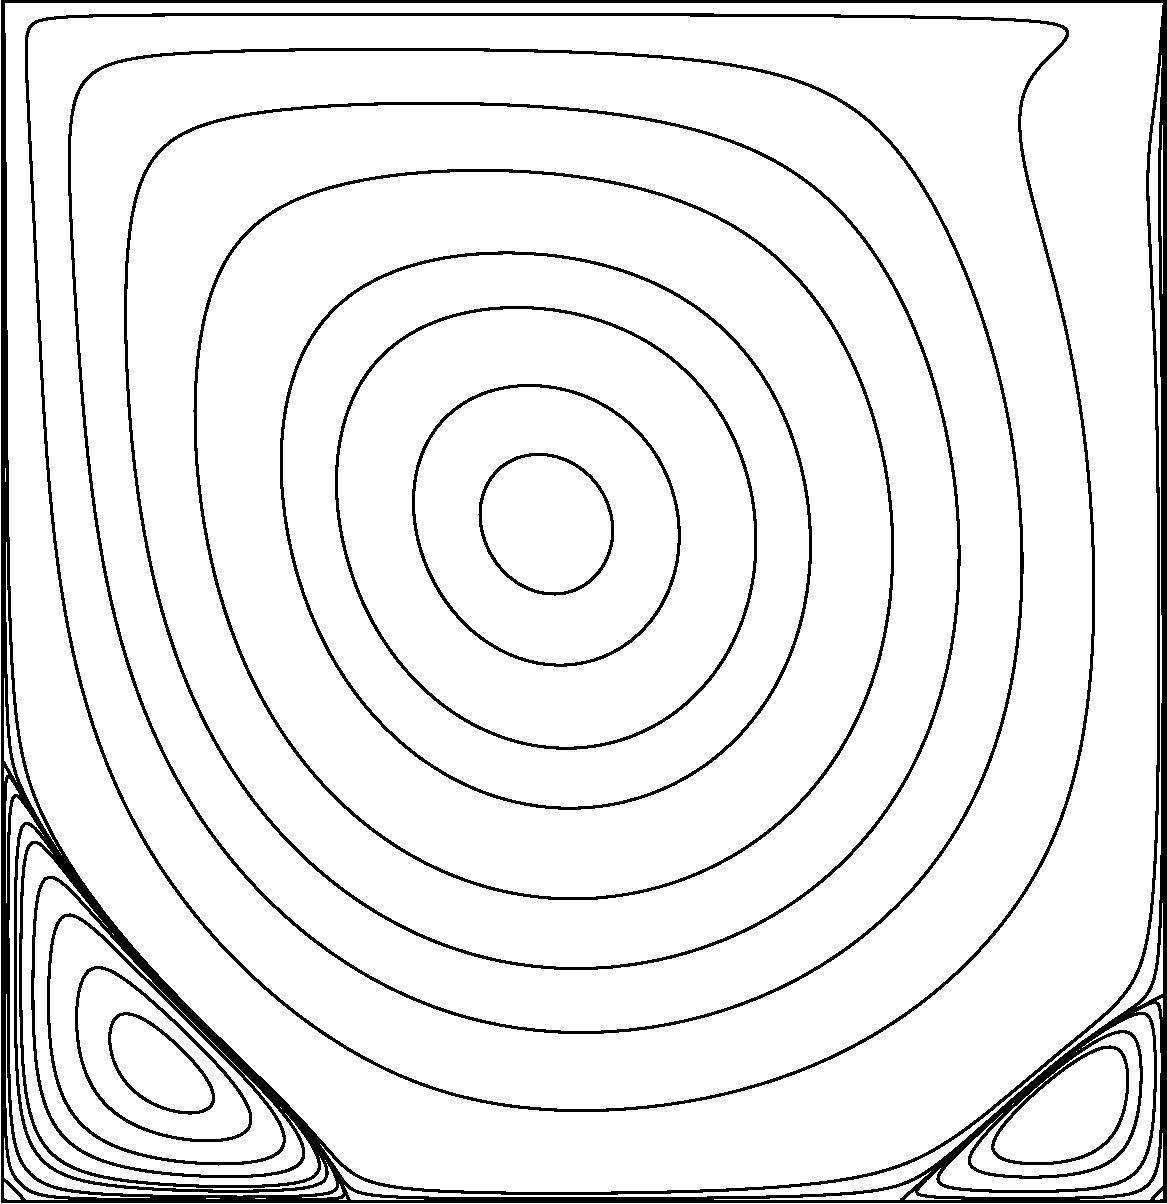
\includegraphics[width=0.8\linewidth]{Images/streamFunction.pdf}\vspace{1.5cm}}
\author{Michel Robijns (Student ID: 4088018)}
\date{\today}

\maketitle

\tableofcontents

\chapter{Objective}

Most of the established numerical methods for discretizing and solving partial differential equations (for instance, the finite-difference method, the finite-volume method, and the finite-element method) are based on the idea of approximating the derivative terms as closely as possible. This is a valid approach, but it has a number of disadvantages; numerical errors are introduced right from the start and the magnitude of the numerical error is a  function of the density of the mesh.  

The objective of this report is to present a novel method for solving the incompressible Navier-Stokes equations using tools from discrete exterior calculus (DEC). The method takes a geometric approach in order to preserve the physical relations rather than approximating them. A key ingredient of the idea is to avoid approximating derivatives entirely by expressing the variables as integrated quantities. The method is therefore mathematically exact until the last stages of the process. The method will be used to solve the incompressible Navier-Stokes equations on a two-dimensional lid-driven cavity because the lid-driven cavity flow problem is a classical test problem for the validation of Navier-Stokes codes. The main aim of this report is to demonstrate that the method works and to show its advantages over classical numerical methods.

In Chapter \ref{cha:physics} we will derive the governing equations and formally present the lid-driven cavity flow problem. In Chapter \ref{cha:mathematics} we will introduce the numerical framework in a step-by-step manner. In Chapter \ref{cha:code} we will show the most important excerpt of the program code and look for ways to optimize the code in terms of memory use and execution speed. Finally, in Chapter \ref{cha:results} we will validate the results using a 1997 paper by O.~Botella and R.~Peyret \parencite{botella1998benchmark}.

\chapter{Physics}
\label{cha:physics}

In this chapter, we will derive the governing equations and introduce the domain on which they are imposed, as well as the associated boundary conditions and initial values. The governing equations must be expressed in terms of certain operators for reasons that will be the subject of Chapter \ref{cha:mathematics}. I chose to re-derive the governing equations to understand their origin and to verify their correctness.

\section{The Navier-Stokes Equations}

The Navier-Stokes equations govern the motion of viscous fluids. These equations arise from the application of conservation of mass, conservation of momentum, and conservation of energy to the motion of fluids and build upon the notion that fluids are a continuous medium rather than a set of discrete particles. The so-called convective form of the Navier-Stokes equations for an incompressible Newtonian fluid without the presence of body forces is \parencite[][]{anderson2011fundamentals}:
\begin{flalign}
    \stepcounter{equation}
    \tag{{\theequation}a}
    &\text{Continuity equation:}& \nabla \cdot \mathbf{u} &= 0 && \\
    \tag{{\theequation}b}
    &\text{Momentum equation:}& \frac{\partial \mathbf{u}}{\partial t} + \left( \mathbf{u} \cdot \nabla \right) \mathbf{u} &= - \frac{1}{\rho} \nabla p + \nu \nabla^2 \mathbf{u} &&
\end{flalign}
where $\mathbf{u}$ is the velocity field, $t$ is the time, $\rho$ is the density, $p$ is the pressure field, and $\nu$ is the kinematic viscosity. A more tangible notation of these equations is obtained by writing them in their vector component forms and by utilizing Einstein's summation convention:
\begin{align}
    \stepcounter{equation}
    \tag{{\theequation}a}
    \label{eq:continuityEinstein}
    \frac{\partial u_i}{\partial x_i} &= 0 \\
    \tag{{\theequation}b}
    \label{eq:momentumEinstein}
    \frac{\partial u_i}{\partial t} + u_j \frac{\partial u_i}{\partial x_j} &= - \frac{1}{\rho} \frac{\partial p}{\partial x_i} + \nu \frac{\partial^2 u_i}{\partial x_j^2}
\end{align}
Equations \eqref{eq:continuityEinstein} and \eqref{eq:momentumEinstein} are dimensional. That is, each parameter like $u_i$, $p$, and $\nu$ is expressed in terms of a physical quantity. Non-dimensionalization can reduce the number of free parameters and can help to gain a greater insight into the relative size of the terms present in the equations. The dimensionless parameters are defined as follows:
\begin{align}
    \stepcounter{equation}
    \tag{{\theequation}a}
    \label{eq:nondimu}
    u_i^* &\equiv \frac{u_i}{U} \\
    \tag{{\theequation}b}
    \label{eq:nondimx}
    x_i^* &\equiv \frac{x_i}{L} \\
    \tag{{\theequation}c}
    \label{eq:nondimt}
    t^* &\equiv t \frac{U}{L} \\
    \tag{{\theequation}d}
    \label{eq:nondimp}
    p^* &\equiv \frac{p}{\rho U^2} \\
    \tag{{\theequation}e}
    \label{eq:Re}
    \text{Re} &\equiv \frac{\nu}{UL}
\end{align}
where $U$ is the velocity scale and $L$ is the length scale of the flow. 

Multiplication of Equations \eqref{eq:continuityEinstein} and \eqref{eq:momentumEinstein} by $L / U$ and $L / U^2$, respectively, gives
\begin{align}
    \stepcounter{equation}
    \tag{{\theequation}a}
    \label{eq:NS1}
    \frac{L}{U} \frac{\partial u_i}{\partial x_i} &= 0 \\
    \tag{{\theequation}b}
    \label{eq:NS2}
    \frac{L}{U^2} \frac{\partial u_i}{\partial t} + \frac{L}{U^2} u_j \frac{\partial u_i}{\partial x_j} &= - \frac{L}{U^2} \frac{1}{\rho} \frac{\partial p}{\partial x_i} + \frac{L}{U^2} \nu \frac{\partial^2 u_i}{\partial x_j^2}
\end{align}
Rearrangement of Equations \eqref{eq:NS1} and \eqref{eq:NS2} yields
\begin{align}
    \stepcounter{equation}
    \tag{{\theequation}a}
    \label{eq:NS3}
    \frac{\partial \frac{u_i}{U}}{\partial \frac{x_i}{L}} &= 0 \\
    \tag{{\theequation}b}
    \label{eq:NS4}
    \frac{\partial \frac{u_i}{U}}{\partial t \frac{U}{L}} + \frac{u_j}{U} \frac{\partial \frac{u_i}{U}}{\partial \frac{x_j}{L}} &= - \frac{1}{\rho} \frac{\partial \frac{p}{U^2}}{\partial \frac{x_i}{L}} + \frac{\nu}{UL} \frac{\partial^2 \frac{u_i}{U}}{\partial \frac{x_j}{L} \partial \frac{x_j}{L}}
\end{align}
Substituting Equations \eqref{eq:nondimu}--\eqref{eq:Re} into Equations \eqref{eq:NS3} and \eqref{eq:NS4}, we obtain
\begin{align}
    \stepcounter{equation}
    \tag{{\theequation}a}
    \frac{\partial u_i^*}{\partial x_i^*} &= 0 \\
    \tag{{\theequation}b}
    \frac{\partial u_i^*}{\partial t^*} + u_j^* \frac{\partial u_i^*}{\partial x_j^*} &= - \frac{\partial p^*}{\partial x_i^*} + \frac{1}{\text{Re}} \frac{\partial^2 u_i^*}{\partial x_j^* \partial x_j^*}
\end{align}
or
\begin{flalign}
    \stepcounter{equation}
    \tag{{\theequation}a}
    & & \nabla \cdot \mathbf{u}^* &= 0 && \\
    \tag{{\theequation}b}
    & & \frac{\partial \mathbf{u}^*}{\partial t^*} + \left( \mathbf{u}^* \cdot \nabla \right) \mathbf{u}^* &= - \nabla p^* + \frac{1}{\text{Re}} \nabla^2 \mathbf{u}^* &&
\end{flalign}
Because it is now understood that the governing equations are dimensionless, the asterisk will be omitted in the remainder of this report. Thus,
\begin{align}
    \stepcounter{equation}
    \tag{{\theequation}a}
    \nabla \cdot \mathbf{u} &= 0 \label{eq:continuity} \\
    \tag{{\theequation}b}
    \frac{\partial \mathbf{u}}{\partial t} + \left( \mathbf{u} \cdot \nabla \right) \mathbf{u} &= - \nabla p + \frac{1}{\text{Re}} \nabla^2 \mathbf{u} \label{eq:momentum}
\end{align}
For reasons that will be the subject of Chapter \ref{cha:mathematics}, it is convenient to rewrite the Navier-Stokes equations in terms of the divergence, curl, and gradient operators. Consider the following vector identities: if $\mathbf{u}$ is a three-dimensional vector field, then
\begin{flalign}
    & & \nabla^2 \mathbf{u} &= \nabla \left( \nabla \cdot \mathbf{u} \right) - \nabla \times \left( \nabla \times \mathbf{u} \right) && \\
    &\text{and}& \left( \mathbf{u} \cdot \nabla \right) \mathbf{u} &= \nabla \left( \frac{1}{2} \left\Vert \mathbf{u} \right\Vert^2 \right) - \mathbf{u} \times \left( \nabla \times \mathbf{u} \right) &&
\end{flalign}
Using these vector identities, Equation \eqref{eq:momentum} can be written as
\begin{equation}
    \label{eq:momentumIdentity}
    \frac{\partial \mathbf{u}}{\partial t} + \nabla \left( \frac{1}{2} \left\Vert \mathbf{u} \right\Vert^2 \right) - \mathbf{u} \times \left( \nabla \times \mathbf{u} \right) = - \nabla p + \frac{1}{\text{Re}} \left( \nabla \left( \nabla \cdot \mathbf{u} \right) - \nabla \times \left( \nabla \times \mathbf{u} \right) \right)
\end{equation}
Recall that in a velocity field, the curl of the velocity is equal to the vorticity:
\begin{equation}
    \label{eq:vorticity}
    \mathbf{\xi} = \nabla \times \mathbf{u}
\end{equation}
Substituting Equation \eqref{eq:vorticity} into Equation \eqref{eq:momentumIdentity}, we have
\begin{equation}
    \label{eq:momentumRearranged1}
    \frac{\partial \mathbf{u}}{\partial t} + \nabla \left( \frac{1}{2} \left\Vert \mathbf{u} \right\Vert^2 \right) - \mathbf{u} \times \xi = - \nabla p + \frac{1}{\text{Re}} \left( \nabla \left( \nabla \cdot \mathbf{u} \right) - \nabla \times \xi \right)
\end{equation}
Some algebraic rearrangement of Equation \eqref{eq:momentumRearranged1} yields
\begin{equation}
    \label{eq:momentumRearranged2}
    \frac{\partial \mathbf{u}}{\partial t} - \mathbf{u} \times \xi + \nabla \left( p + \frac{1}{2} \left\Vert \mathbf{u} \right\Vert^2 \right) = \frac{1}{\text{Re}} \left( \nabla \left( \nabla \cdot \mathbf{u} \right) - \nabla \times \xi \right)
\end{equation}
In Equation \eqref{eq:momentumRearranged2}, denote
\begin{equation}
    P \equiv p + \frac{1}{2} \left\Vert \mathbf{u} \right\Vert^2
\end{equation}
and recognize that the continuity equation, $\nabla \cdot \mathbf{u} = 0$, appears in the right-hand side. Hence, Equation \eqref{eq:momentumRearranged2} is written as
\begin{equation}
    \frac{\partial \mathbf{u}}{\partial t} - \mathbf{u} \times \xi + \nabla P + \frac{1}{\text{Re}} \nabla \times \xi = 0
\end{equation}
Thus, the final system of equations is given by:
\begin{flalign}
    \stepcounter{equation}
    \tag{{\theequation}a}
    &\text{Continuity equation:}& &\vphantom{\frac{\partial}{\partial}} \nabla \cdot \mathbf{u} = 0 && \\
    \tag{{\theequation}b}
    &\text{Velocity-vorticity relation:}& &\vphantom{\frac{\partial}{\partial}} \xi = \nabla \times \mathbf{u} && \\
    \tag{{\theequation}c}
    &\text{Momentum equation:}& &\frac{\partial \mathbf{u}}{\partial t} - \mathbf{u} \times \xi + \nabla P + \frac{1}{\text{Re}} \nabla \times \xi = 0 &&
\end{flalign}

\section{The Lid-Driven Cavity Flow Problem}

The incompressible dimensionless Navier-Stokes equations will be solved on the two-dimensional square domain $\Omega \equiv \left[ 0, 1 \right] \times \left[ 0, 1 \right]$, shown in Figure \ref{fig:problem}. The boundary of $\Omega$ is defined as 
\begin{equation}
    \partial \Omega \equiv \Gamma_1 \cup \Gamma_2 \cup \Gamma_3 \cup \Gamma_4 
\end{equation}

The top boundary or "lid" of $\Omega$, $\Gamma_3$, imposes a shear stress on the fluid by moving leftward with a velocity of unity, hence the name lid-driven cavity flow problem. Thus, the boundary conditions are $\left. \mathbf{u} \right|_{\Gamma_3} = (-1, 0)$ and $\left. \mathbf{u} \right|_{\Gamma_1} = \left. \mathbf{u} \right|_{\Gamma_2} = \left. \mathbf{u} \right|_{\Gamma_4} = (0, 0)$. At $t = 0$, the fluid is at rest. That is, $ \left. \mathbf{u} \right|_{t = 0} = 0$.

\begin{figure}[ht]
    \centering
    \begin{tikzpicture}
        % Draw lines
        \foreach \i in {0,5} {
            \draw (\i,0) -- (\i,5);
            \draw (0,\i) -- (5,\i);
        }
        % Draw x-axis and y-axis
        \draw [dashed, ->] (5,0) -- (6,0) node [right] {x};
        \draw [dashed, ->] (0,5) -- (0,6) node [above] {y};
        % Label corner points
        \node[below left=1ex] at (0,0) {$0$};
        \node[below=1ex] at (5,0) {$1$};
        \node[left=1ex] at (0,5) {$1$};
        % Label domain
        \node at (2.5,2.5) {$\Omega$};
        % Label boundaries
        \node[above=1ex] at (2.5,5) {$\Gamma_3$};
        \node[below=1ex] at (2.5,0) {$\Gamma_1$};
        \node[left=1ex] at (0,2.5) {$\Gamma_4$};
        \node[right=1ex] at (5,2.5) {$\Gamma_2$};
    \end{tikzpicture}
    \caption{The lid-driven cavity flow problem.}
    \label{fig:problem}
\end{figure}


\chapter{Mathematics}
\label{cha:mathematics}

In Chapter \ref{cha:physics} we derived a system of dimensionless partial differential equations that govern the motion of viscous fluids. In this chapter, we cover some mathematical machinery to formulate the problem into a format understandable by a computer. Instead of using classical discretization methods like the finite difference method, we take a geometric approach using tools from discrete exterior calculus (DEC). A key ingredient in this geometric approach is the placement of physical quantities on the appropriate geometric structures. DEC is a vast mathematical field and a rigorous treatment is far beyond the scope of this assignment. The scope of this chapter is therefore limited to those particular concepts that are required to solve the lid-driven cavity flow problem.

\section{Cells}

Let us first introduce a discrete version of two-dimensional space. Two-dimensional space supports geometric structures with either zero, one, or two dimensions: points, lines, and planes. These $k$-dimensional geometric structures are formally called $k$-cells, denoted $\sigma^{(k)}$, where $k$ represents the dimension of the cell. Three examples of $k$-cells are shown in Figure \ref{fig:cells}.
\begin{figure}[h]
    \newsavebox\boxCell
    \savebox{\boxCell}{\begin{tikzpicture}
        \fill (0,0) circle (0.03);
        \fill (2,0) circle (0.03);
        \fill (2,2) circle (0.03);
        \fill (0,2) circle (0.03);
        \draw (0,0) .. controls (0.5,0.25) and (1.5,-0.25) .. (2,0) .. controls (1.75,0.5) and (2.25,1.5) .. (2,2) .. controls (1.5,1.75) and (0.5,2.25) .. (0,2) .. controls (0.25,1.5) and (-0.25,0.5) .. (0,0);
    \end{tikzpicture}}
    \centering
    \begin{subfigure}[c]{0.3\textwidth}
        \centering
        \vbox to \ht\boxCell{
            \vfill
            \begin{tikzpicture}
                \fill (1,1) circle (0.03);
            \end{tikzpicture}
            \vfill
        }
        \caption{0-cell (point)}
    \end{subfigure}
    \begin{subfigure}[c]{0.3\textwidth}
        \centering
        \vbox to \ht\boxCell{
            \vfill
            \begin{tikzpicture}
                \fill (0,1) circle (0.03);
                \draw (0,1) .. controls (0.5,1.25) and (1.5,0.75) .. (2,1);
                \fill (2,1) circle (0.03);
            \end{tikzpicture}
            \vfill
        }
        \caption{1-cell (line)}
    \end{subfigure}
    \begin{subfigure}[c]{0.3\textwidth}
        \centering
        \usebox{\boxCell}
        \caption{2-cell (plane)}
        \label{fig:2cell}
    \end{subfigure}
    \caption{Examples of $k$-cells in two-dimensional space.}
    \label{fig:cells}
\end{figure}

A point is a 0-cell, a line is a 1-cell, and a plane is a 2-cell. Just like a 1-cell is a line with a length but with no position, a 2-cell can be thought of as a plane with an area, but no position. Notice that $k$-cells are bounded by $(k-1)$-cells and that a cell's shape is arbitrary, as indicated by the wavy lines. (\textit{Note:} The boundary of a point is empty by definition.)

We will be using points, lines, and planes as building blocks of our mesh. A mesh is a set of cells, called a cell-complex if the boundary of each cell is also part of the set. For example, the (rather primitive) mesh in Figure \ref{fig:2cell} is a cell-complex because the plane is bounded by lines and the lines are in turn bounded by points, all of which are part of the mesh.

\section{Chains and Cochains}

There are two additional concepts that require some elaboration: the notion of $k$-chains and the notion of $k$-cochains. A $k$-chain is essentially a set of $k$-cells. That is, nothing more and nothing less than a set of geometric structures \emph{of the same dimension}. For instance, a set of lines or a set of planes. $k$-cochains build upon chains; a $k$-cochain is essentially a set of $k$-cells tagged with a numerical value. $k$-cochains are in practice realized as a vector of single or double precision numbers and it may help to think of $k$-cochains as such. Rigorous definitions of chains and cochains can be found in \parencite{gerritsma2014computational}.
 
\section{Orientation}

In addition to dimension, $k$-cells have a property called orientation. A $k$-cell either has a positive or a negative orientation that can be freely chosen per individual cell, as long as its orientation remains unchanged thereafter. However, in practice it may be a good idea to define an orientation that is consistent throughout all $k$-cells.

Figure \ref{fig:innerExample} shows three $k$-cells in two-dimensional space with an intrinsic orientation that we call inner-oriented $k$-cells. Inner-oriented points for instance, can either represent sources or sinks and are arbitrarily chosen to be source-like (that it, an outflow is positive), as indicated by the outward pointing arrows in Figure \ref{fig:inner0Cell}. Inner-oriented lines are chosen to be a positive when pointing to the right, as indicated by the arrow in Figure \ref{fig:inner1Cell}. It is somewhat awkward to think of the orientation of a plane, but an inner-oriented plane is defined as positive when it is oriented counterclockwise, as indicated by the curled arrow in Figure \ref{fig:inner2Cell}.
\begin{figure}[h]
    \newsavebox\boxInner
    \savebox{\boxInner}{\begin{tikzpicture}
        \draw (0,0) .. controls (0.5,0.25) and (1.5,-0.25) .. (2,0) .. controls (1.75,0.5) and (2.25,1.5) .. (2,2) .. controls (1.5,1.75) and (0.5,2.25) .. (0,2) .. controls (0.25,1.5) and (-0.25,0.5) .. (0,0) -- cycle;
        \draw [->] (1,1) ++(140:0.25) arc (-220:40:0.25);
    \end{tikzpicture}}
    \centering
    \begin{subfigure}[c]{0.3\textwidth}
        \centering
        \vbox to \ht\boxInner{
            \vfill
            \begin{tikzpicture}
                \fill (1,1) circle (0.03);
                \draw [->] (1,1.075) -- (1,1.25);
                \draw [->] (1.075,1) -- (1.25,1);
                \draw [->] (1,0.925) -- (1,0.75);
                \draw [->] (0.925,1) -- (0.75,1);
            \end{tikzpicture}
            \vfill
        }
        \caption{0-cell}
        \label{fig:inner0Cell}
    \end{subfigure}
    \begin{subfigure}[c]{0.3\textwidth}
        \centering
        \vbox to \ht\boxInner{
            \vfill
            \begin{tikzpicture}
                \draw (0,1) .. controls (0.5,1.25) and (1.5,0.75) .. (2,1);
                \draw [->] (0.95,1.008) -- (1.05,0.992);
            \end{tikzpicture}
            \vfill
        }
        \caption{1-cell}
        \label{fig:inner1Cell}
    \end{subfigure}
    \begin{subfigure}[c]{0.3\textwidth}
        \centering
        \centering
        \usebox{\boxInner}
        \caption{2-cell}
        \label{fig:inner2Cell}
    \end{subfigure}
    \caption{Inner-oriented $k$-cells in two-dimensional space.}
    \label{fig:innerExample}
\end{figure}
\begin{figure}[h]
    \newsavebox\outerBox
    \savebox{\outerBox}{\begin{tikzpicture}
        \draw (0,0) .. controls (0.5,0.25) and (1.5,-0.25) .. (2,0) .. controls (1.75,0.5) and (2.25,1.5) .. (2,2) .. controls (1.5,1.75) and (0.5,2.25) .. (0,2) .. controls (0.25,1.5) and (-0.25,0.5) .. (0,0) -- cycle;
        \draw [->] (1,1.075) -- (1,1.25);
        \draw [->] (1.075,1) -- (1.25,1);
        \draw [->] (1,0.925) -- (1,0.75);
        \draw [->] (0.925,1) -- (0.75,1);
    \end{tikzpicture}}
    \centering
    \begin{subfigure}[c]{0.3\textwidth}
        \centering
        \vbox to \ht\outerBox{
            \vfill
            \begin{tikzpicture}
                \fill (1,1) circle (0.03);
                \draw [->] (1,1) ++(140:0.25) arc (-220:40:0.25);
            \end{tikzpicture}
            \vfill
        }
        \caption{0-cell}
    \end{subfigure}
    \begin{subfigure}[c]{0.3\textwidth}
        \centering
        \vbox to \ht\outerBox{
            \vfill
            \begin{tikzpicture}
                \draw (0,1) .. controls (0.5,1.25) and (1.5,0.75) .. (2,1);
                \draw [->] (0.96,0.75) -- (1.04,1.25);
            \end{tikzpicture}
            \vfill
        }
        \caption{1-cell}
    \end{subfigure}
    \begin{subfigure}[c]{0.3\textwidth}
        \centering
        \usebox{\outerBox}
        \caption{2-cell}
    \end{subfigure}
    \caption{Outer-oriented $k$-cells in two-dimensional space.}
    \label{fig:outerExample}
\end{figure}

Inner-oriented $k$-cells have outer-oriented counterparts with an circumcentric orientation, rather than an intrinsic orientation. For example, the orientation of an inner-oriented line is defined \emph{on} that line whereas the orientation of an outer-oriented line is defined \emph{through} that line. Figure \ref{fig:outerExample} shows three outer-oriented $k$-cells in two-dimensional space.

The distinction between inner and outer-oriented $k$-cells is justified from a physical of view; certain physical quantities are naturally expressed in terms of inner-oriented cochains whereas other physical quantities are naturally expressed in terms of outer-oriented cochains.

\section{The Exterior Derivative}

The exterior derivative $\delta$ is used to compute derivatives, like gradients, divergences, or curls. The descrete exterior derivative is a linear map from a $(k)$-cochain to a $(k+1)$-cochain. It turns out that the standard treatment of vector calculus hides a number of important things that are applied implicitly. As shall be seen in the upcoming examples, all three of the multivariable derivatives in vector calculus (i.e. gradients, curls, and divergences) are actually \emph{one} kind of derivative: the exterior derivative. The exterior derivative will be introduced by means of examples to provide a suitable context for the discussion of the physical interpretation of $k$-cochains.

\subsection{Inner-Oriented Quantities}

To capture the geometric structure of the governing equations, we define its physical quantities through integral values over the elements of the mesh. Depending on whether a given physical quantity is a point, line, or area density, its corresponding discrete representation ``lives'' at the associated zero, one, or two dimensional mesh elements.

We would eventually like to know the velocity field within the domain of our problem. We use circulation, i.e., the line integral of the velocity field, to encode velocity on the mesh elements. Let inner-oriented 1-cochains therefore represent circulation, defined as
\begin{flalign}
    \stepcounter{equation}
    \tag{{\theequation}a}
    & & u_{i,j} \equiv \int_L \mathbf{u} \cdot  \mathbf{\hat{t}} \, dx && \\
    \tag{{\theequation}b}
    &\text{and}& v_{i,j} \equiv \int_L \mathbf{u} \cdot \mathbf{\hat{t}} \, dy &&
\end{flalign}
where $\mathbf{\hat{t}}$ denotes the tangent vector along a line and where the notations $u$ and $v$ are reserved for horizontal and vertical lines, respectfully. It is crucial to note that this makes circulation an \emph{integrated}, not pointwise, quantity. Thus, the physical quantity of circulation ``lives'' at the one-dimensional mesh elements (i.e., lines).

\begin{figure}[h]
    \newsavebox\boxExample
    \savebox{\boxExample}{\begin{tikzpicture}
        \fill (0,0) circle (0.03) node [below left=0.5ex] at (1,0) {3} node [below right=0.5ex] at (1,0) {$L_1$};
        \fill (2,0) circle (0.03) node [below right=0.5ex] at (2,1) {7} node [above right=0.5ex] at (2,1) {$L_2$};
        \fill (2,2) circle (0.03) node [above left=0.5ex] at (1,2) {$-5$} node [above right=0.5ex] at (1,2) {$L_3$};
        \fill (0,2) circle (0.03) node [below left=0.5ex] at (0,1) {9} node [above left=0.5ex] at (0,1) {$L_4$};
        \draw (0,0) .. controls (0.5,0.25) and (1.5,-0.25) .. (2,0) .. controls (1.75,0.5) and (2.25,1.5) .. (2,2) .. controls (1.5,1.75) and (0.5,2.25) .. (0,2) .. controls (0.25,1.5) and (-0.25,0.5) .. (0,0) -- cycle;
        \draw [->] (1,1) ++(140:0.25) arc (-220:40:0.25) node [above left=1ex] at (1,1) {6} node [below right=1ex] at (1,1) {$S$};
        \draw [->] (0.95,0.008) -- (1.05,-0.008);
        \draw [->] (1.992,0.95) -- (2.008,1.05);
        \draw [->] (0.95,2.008) -- (1.05,1.992);
        \draw [->] (-0.008,0.95) -- (0.008,1.05);
    \end{tikzpicture}}
    \centering
    \begin{subfigure}[c]{0.3\textwidth}
        \centering
        \vbox to \ht\boxExample{
            \vfill
            \begin{tikzpicture}
                \fill (1,1) circle (0.03) node [above left=0.5ex] {8} node [below right=0.5ex] {$p_0$};
                \draw [->] (1,1.075) -- (1,1.25);
                \draw [->] (1.075,1) -- (1.25,1);
                \draw [->] (1,0.925) -- (1,0.75);
                \draw [->] (0.925,1) -- (0.75,1);
            \end{tikzpicture}
            \vfill
        }
        \caption{0-cochain}
        \label{fig:0cochainExample}
    \end{subfigure}
    \begin{subfigure}[c]{0.3\textwidth}
        \centering
        \vbox to \ht\boxExample{
            \vfill
            \begin{tikzpicture}
                \fill (0,1) circle (0.03) node [above left=0.5ex] {4};
                \fill (0,1) circle (0.03) node [below left=0.5ex] {$p_1$};
                \draw (0,1) .. controls (0.5,1.25) and (1.5,0.75) .. (2,1);
                \fill (2,1) circle (0.03) node [above right=0.5ex] {6};
                \fill (2,1) circle (0.03) node [below right=0.5ex] {$p_2$};
                \draw [->] (0.95,1.008) -- (1.05,0.992) node [above=0.5ex] at (1,1) {$-2$} node [below=0.5ex] at (1,1) {$L_0$};
            \end{tikzpicture}
            \vfill
        }
        \caption{1-cochain}
        \label{fig:1cochainExample}
    \end{subfigure}
    \begin{subfigure}[c]{0.3\textwidth}
        \centering
        \usebox{\boxExample}
        \caption{2-cochain}
        \label{fig:2cochainExample}
    \end{subfigure}
    \caption{Examples of $k$-cochains in two-dimensional space.}
    \label{fig:cochainExamples}
\end{figure}

Figure \ref{fig:cochainExamples} shows three examples of inner-oriented $k$-cochains in two-dimensional space. Recall that cochains can be thought of as chains tagged with a number, hence the numerical values in Figure \ref{fig:cochainExamples}. Figure \ref{fig:1cochainExample} shows a 0-cochain consisting of two points, $p_1$ and $p_2$, and a 1-cochain composed of a line, $L_0$. $L_0$ points from $p_1$ to $p_2$, so $p_1$ acts as a source and $p_2$ acts as a sink. The recipe for applying $\delta$ is straightforward: simply add values at points that act as a source and subtract values at points that act as a sink. Because points are source-like by default, as indicated in Figure \ref{fig:0cochainExample}, application of $\delta$ results in
\begin{equation}
    u = \delta(L_0) = 4 - 6 = -2
\end{equation}

Assuming that points represent samples of a continuous scalar field, $P$, it is clearly seen that the application of $\delta$ on a 0-cochain is analogous to the \emph{integrated} gradient operator:
\begin{equation}
    \begin{split}
        4 - 6 &= P(p_2) - P(p_1) \\
        &= \int_{L} \nabla \phi \cdot \mathbf{ds}
    \end{split}
\end{equation}
$P$ can be interpreted of as a dimensionless version of total pressure ($P \equiv p + \frac{1}{2}||\mathbf{u}||^2$).

Figure \ref{fig:2cochainExample} shows a 1-cochain composed of four lines and a 2-cochain composed of a single plane, $S$. We apply the discrete exterior derivative by either adding or subtracting the line values; if the orientation of a line segment opposes the orientation of the plane, then its value must be subtracted. Thus, application of $\delta$ on $S$ results in\begin{equation}
    \xi = \delta(S) = 3 + 7 - (-5) - 9 = 6
\end{equation}

Application of $\delta$ on a 1-cochain is analogous to the integrated curl operator because\begin{equation}
    \begin{split}
        3 + 7 - (-5) - 9 &= u_1(L_1) + v_2(L_2) - u_2(L_3) - v_1(L_4) \\
        &= \int_{L_1} \mathbf{u} \cdot \mathbf{dl} + \int_{L_2} \mathbf{u} \cdot \mathbf{dl} - \int_{L_3} \mathbf{u} \cdot \mathbf{dl} - \int_{L_4} \mathbf{u} \cdot \mathbf{dl} \\
        &= \oint_{\partial S} \mathbf{u} \cdot \mathbf{dl} \\
        &= \iint_{S} \left( \nabla \times \mathbf{u} \right) \cdot dA
    \end{split}
    \label{eq:vorticityExample}
\end{equation}
where $\partial S \equiv L_1 \cup L_2 \cup L_3 \cup L_4$. This is not the only insight to be gained here; recall that the circulation along a closed contour, denoted $\Gamma$, is defined as:
\begin{equation}
    \Gamma \equiv \oint_C \mathbf{u} \cdot \mathbf{dl}
    \label{eq:circulation}
\end{equation}
Comparing Equations \eqref{eq:vorticityExample} and \eqref{eq:circulation}, we conclude that $\delta(S)$ must represent the circulation around the edges of $S$. Circulation is related to vorticity; the circulation around a closed contour is equal to the integrated vorticity enclosed by that contour. From Stokes' theorem:
\begin{equation}
    \Gamma \equiv \oint_C \mathbf{u} \cdot \mathbf{dl} = \iint_A \left( \nabla \times \mathbf{u} \right) dA = \iint_A \xi \; dA
\end{equation}
Inner-oriented 2-cochains $\xi$ can therefore be interpreted as vorticity.

Because $3$-cochains are undefined in two-dimensional space, the application of $\delta$ on a 2-cochain results in the empty set by definition. In a similar vein, 0-cochains can only be the result of the application of $\delta$ on a real number \parencite{hirani2003discrete}.

\subsection{Outer-Oriented Quantities}

We use flux, i.e., the integral of the normal velocity along a line, as a representation of velocity on an outer-oriented mesh. Note again that this makes flux an integrated, not pointwise, quantity. Thus, let the outer-oriented 1-cochains represent flux, defined as
\begin{flalign}
    \stepcounter{equation}
    \tag{{\theequation}a}
    & & \tilde{u}_{i,j} \equiv \int_L \mathbf{u} \cdot  \mathbf{\hat{n}} \, dy && \\
    \tag{{\theequation}b}
    &\text{and}& \tilde{v}_{i,j} \equiv \int_L \mathbf{u} \cdot \mathbf{\hat{n}} \, dx &&
\end{flalign}
where $\mathbf{\hat{n}}$ denotes the normal vector along the line segment and where $u_{i,j}$ and $v_{i,j}$ are again reserved for horizontal and vertical lines, respectively.
All outer-oriented geometric structures and quantities are marked with a tilde for easy recognition. Figure \ref{fig:outerCochainExamples} shows three examples of outer-oriented $k$-cochains in two-dimensional space.

\begin{figure}[ht]
    \newsavebox\boxOuterExample
    \savebox{\boxOuterExample}{\begin{tikzpicture}
        \fill (0,0) circle (0.03) node [below left=0.5ex] at (1,0) {3} node [below right=0.5ex] at (1,0) {$\tilde{L}_1$};
        \fill (2,0) circle (0.03) node [below right=0.5ex] at (2,1) {7} node [above right=0.5ex] at (2,1) {$\tilde{L}_2$};
        \fill (2,2) circle (0.03) node [above left=0.5ex] at (1,2) {$-5$} node [above right=0.5ex] at (1,2) {$\tilde{L}_3$};
        \fill (0,2) circle (0.03) node [below left=0.5ex] at (0,1) {9} node [above left=0.5ex] at (0,1) {$\tilde{L}_4$};
        \draw (0,0) .. controls (0.5,0.25) and (1.5,-0.25) .. (2,0) .. controls (1.75,0.5) and (2.25,1.5) .. (2,2) .. controls (1.5,1.75) and (0.5,2.25) .. (0,2) .. controls (0.25,1.5) and (-0.25,0.5) .. (0,0) -- cycle;
        \node [above left=0.5ex] at (1,1) {$-10$};
        \node [below right=0.5ex] at (1,1) {$\tilde{S}$};
        \draw [->] (0.96,-0.25) -- (1.04,0.25);
        \draw [->] (1.75,1.04) -- (2.25,0.96);
        \draw [->] (0.96,1.75) -- (1.04,2.25);
        \draw [->] (-0.25,1.04) -- (0.25,0.96);
        \draw [->] (1,1.075) -- (1,1.25);
        \draw [->] (1.075,1) -- (1.25,1);
        \draw [->] (1,0.925) -- (1,0.75);
        \draw [->] (0.925,1) -- (0.75,1);
    \end{tikzpicture}}
    \centering
    \begin{subfigure}[c]{0.3\textwidth}
        \centering
        \vbox to \ht\boxOuterExample{
            \vfill
            \begin{tikzpicture}
                \fill (1,1) circle (0.03) node [above left=1ex] {8} node [below right=1ex] {$\tilde{p}_0$};
                \draw [->] (1,1) ++(140:0.25) arc (-220:40:0.25);
            \end{tikzpicture}
            \vfill
        }
        \caption{0-cochain}
        \label{fig:outer0CochainExample}
    \end{subfigure}
    \begin{subfigure}[c]{0.3\textwidth}
        \centering
        \vbox to \ht\boxOuterExample{
            \vfill
            \begin{tikzpicture}
                \draw [->] (0,1) ++(100:0.25) arc (-260:0:0.25);
                \draw [->] (2,1) ++(280:0.25) arc (-80:180:0.25);
                \fill (0,1) circle (0.03) node [above left=1ex] {4};
                \fill (0,1) circle (0.03) node [below left=1ex] {$\tilde{p}_1$};
                \draw (0,1) .. controls (0.5,1.25) and (1.5,0.75) .. (2,1);
                \fill (2,1) circle (0.03) node [above right=1ex] {6};
                \fill (2,1) circle (0.03) node [below right=1ex] {$\tilde{p}_2$};
                \draw [->] (0.96,0.75) -- (1.04,1.25) node [above left=1ex] at (1,1) {$-2$} node [below right=1ex] at (1,1) {$\tilde{L}_0$};
            \end{tikzpicture}
            \vfill
        }
        \caption{1-cochain}
        \label{fig:outer1CochainExample}
    \end{subfigure}
    \begin{subfigure}[c]{0.3\textwidth}
        \centering
        \usebox{\boxOuterExample}
        \caption{2-cochain}
        \label{fig:outer2CochainExample}
    \end{subfigure}
    \caption{Examples of $k$-cochains in two-dimensional space.}
    \label{fig:outerCochainExamples}
\end{figure}

Figure \ref{fig:outer1CochainExample} shows a 0-cochain composed of two points, $\tilde{p}_1$ and $\tilde{p}_2$, and a 1-cochain composed of a line, $\tilde{L}_0$. The recipe for applying $\delta$ is again  straightforward: add values at points that share a common orientation with the line and subtract values whose orientation opposes the orientation of the line. The orientation of $\tilde{p}_2$, for example, opposes the orientation of $\tilde{L}_0$ because the arrows point in opposite directions. Thus,\begin{equation}
    \tilde{u} = \delta(\tilde{L}_0) = 4 - 6 = -2
\end{equation}
This procedure is analogous to the integrated gradient operator because
\begin{equation}
    \begin{split}
        4 - 6 &= \tilde{\psi}(p_2) - \tilde{\psi}(p_1) \\
        &= \int_{L} \nabla \tilde{\psi} \cdot \mathbf{ds}
    \end{split}
\end{equation}

Let us consider the physical interpretation of 0-cochains. If lines represent flux, then points must represent the stream function, $\tilde{\psi}$. Here is why: the numerical value of the stream function is defined such that the difference $\Delta \tilde{\psi}$ between two streamlines is equal to the mass flux between the two streamlines. This fact allows us to determine the stream function up to a constant.

Figure \ref{fig:outer2CochainExample} shows an outer-oriented 1-cochain composed of four lines and an outer-oriented 2-cochain composed of a plane, $\tilde{S}$. The plane is source-like as indicated by the outward pointing arrows. We apply the discrete exterior derivative by adding inflows and subtracting outflows. Thus, application of $\delta$ yields
\begin{equation}
    \tilde{\xi} = \delta(\tilde{S}) = -3 + 7 - 5 - 9 = -10
\end{equation}

The application of $\delta$ on a 1-cochain is analogous to the integrated curl operator because
\begin{equation}
    \begin{split}
        -3 + 7 + (-5) - 9 &= -\tilde{u}_1(\tilde{L}_1) + \tilde{v}_2(\tilde{L}_2) + \tilde{u}_2(\tilde{L}_3) - \tilde{v}_1(\tilde{L}_4) \\
        &= -\int_{\tilde{L}_1} \mathbf{u} \cdot \mathbf{dl} + \int_{\tilde{L}_2} \mathbf{u} \cdot \mathbf{dl} + \int_{\tilde{L}_3} \mathbf{u} \cdot \mathbf{dl} - \int_{\tilde{L}_4} \mathbf{u} \cdot \mathbf{dl} \\
        &= \oint_{\partial \tilde{S}} \mathbf{u} \cdot \mathbf{dl} \\
        &= \iint_{\tilde{S}} \left( \nabla \times \mathbf{u} \right) \cdot dA
    \end{split}
    \label{eq:curlExample}
\end{equation}
where $\partial \tilde{S} \equiv \tilde{L}_1 \cup \tilde{L}_2 \cup \tilde{L}_3 \cup \tilde{L}_4$. 

What is the physical interpretation of $\tilde{\xi}$? The fluid is incompressible, so the velocity field must be divergence free (i.e., $\nabla \cdot \mathbf{u} = 0$). According to the generalized Stokes' theorem the integral of the divergence over a plane equals the sum of the fluxes on all its four edges. In other words, everything that gets in must also get out. The 2-cochain $\tilde{\xi}$ therefore represents the rate of mass production in the plane at which it ``lives''. Thus, for the law of mass conservation to hold true, $\tilde{\xi}$ must be equal to zero at each and every plane because the problem is incompressible.

\subsection{DeRham Complex}

A major advantage of the discrete exterior derivative is that it satisfies the same rules and identities as its smooth counterpart. The discrete exterior derivative is mathematically exact because it acts on and produces integrated quantities. That is, application of $\delta$ does not introduce any error whatsoever. As we shall see, this property contributes to the strength of the geometric approach and it results in preservation of the physics implied in the smooth governing equations. The results of this section can be summarized in a diagram called the DeRham complex \parencite{gerritsma2014computational}:
\begin{equation}
    \begin{gathered}
        \xymatrix@C=20ex{
            C^{(0)} \ar[r]^{\delta}_{\text{grad}} & C^{(1)} \ar[r]^{\delta}_{\text{curl}} & C^{(2)} \\
            \tilde{C}^{(0)} \ar[r]^{\delta}_{\text{grad}} & \tilde{C}^{(1)} \ar[r]^{\delta}_{\text{curl}} & \tilde{C}^{(2)}
        }
    \end{gathered}
\end{equation}

\section{The Hodge-$\star$ Operator}

We have established that two-dimensional space supports points, lines, and planes. Let us briefly digress to three-dimensional space for the sake of familiarity; three-dimensional space supports points, lines, planes, and volumes. In three-dimensional space, we can have one linearly independent volume, three linearly independent planes, three linearly independent lines (just like vectors in $\mathbb{R}^3$), and again one linearly independent point. This 1--3--3--1 sequence suggests a pairing; there exists a vector space isomorphism between $k$-vectors and $(n-k)$-vectors. The Hodge-$\star$ operator is a linear map between inner-oriented $k$-cochains and outer-oriented $(n-k)$-cochains or vice versa, where $n$ denotes the dimension of the vector space. It simply scales the quantities stored on the mesh cells by the size of the corresponding $k$-cells \parencite{elcott2005discrete}.

We have introduced the $\delta$ operator to map $(k)$-cochains to $(k+1)$-cochains. However, the Navier-Stokes equations equate both inner and outer oriented cochains, which requires the Hodge-$\star$ operator. The Hodge-$\star$ operator links the DeRham complices for inner and outer oriented cochains. This linked structure is called the double DeRham complex:
\begin{equation}
    \begin{gathered}
        \xymatrix@=20ex{
            C^{(0)} \ar[r]^{\delta}_{\text{grad}} \ar@{<->}[d]^{\star} & C^{(1)} \ar[r]^{\delta}_{\text{curl}} \ar@{<->}[d]^{\star} & C^{(2)} \ar@{<->}[d]^{\star} \\
            \tilde{C}^{(2)} & \tilde{C}^{(1)} \ar[l]_{\delta}^{\text{curl}} & \tilde{C}^{(0)} \ar[l]_{\delta}^{\text{grad}}
        }
    \end{gathered}
    \label{eq:doubleDeRham}
\end{equation}

In a discrete setting, cochains are stored in vectors, the $\delta$ operator is represented by incidence matrices, denoted $\mathbb{E}$, and the Hodge-$\star$ operator is represented by Hodge matrices, denoted $\mathbb{H}$. In such a framework, application of the $\delta$ or Hodge-$\star$ operator becomes a matrix vector-multiplication. Hence, the double DeRham complex in Equation \eqref{eq:doubleDeRham} becomes
\begin{equation}
    \begin{gathered}
        \xymatrix@=20ex{
            C^{(0)} \ar[r]^{\mathbb{E}^{(1,0)}}_{\text{grad}} \ar@<1ex>[d]^{\mathbb{H}^{(\tilde{2},0)}} & C^{(1)} \ar[r]^{\mathbb{E}^{(2,1)}}_{\text{curl}} \ar@<1ex>[d]^{\mathbb{H}^{(\tilde{1},1)}} & C^{(2)} \ar@<1ex>[d]^{\mathbb{H}^{(\tilde{0},2)}} \\
            \tilde{C}^{(2)} \ar@<1ex>[u]^{\mathbb{H}^{(0,\tilde{2})}} & \tilde{C}^{(1)} \ar[l]_{\tilde{\mathbb{E}}^{(2, 1)}}^{\text{curl}} \ar@<1ex>[u]^{\mathbb{H}^{(1,\tilde{1})}} & \tilde{C}^{(0)} \ar[l]_{\tilde{\mathbb{E}}^{(1,0)}}^{\text{grad}} \ar@<1ex>[u]^{\mathbb{H}^{(2,\tilde{0})}}
        }
    \end{gathered}
\end{equation}

\section{Discretization of the Unit Square}
\label{sec:discretization}

\begin{figure}[ht]
    \centering
    \begin{tikzpicture}
        % Draw scale
        \foreach \ia/\ib/\count in {0/2/0, 2/6/1, 6/8/2} {
            \draw [|<->|] (-1.5,\ia) -- (-1.5,\ib) node [midway,fill=white] {$\tilde{h}_\count$};
            \draw [|<->|] (\ia,-1.5) -- (\ib,-1.5) node [midway,fill=white] {$\tilde{h}_\count$};
        }
        % Draw lines
        \foreach \i in {0,2,6,8} {
            \draw (\i,0) -- (\i,8);
            \draw (0,\i) -- (8,\i);
        }
        % Draw axis
        \draw [dashed, ->] (8,0) -- (9,0) node [right] {x};
        \draw [dashed, ->] (0,8) -- (0,9) node [above] {y};
        % Four courner points
        \fill (0,0) circle (0.03) node [below left=1ex] {$\tilde{\psi}_{0,0}$};
        \fill (8,0) circle (0.03) node [below right=1ex] {$\tilde{\psi}_{3,0}$};
        \fill (8,8) circle (0.03) node [above right=1ex] {$\tilde{\psi}_{3,3}$};
        \fill (0,8) circle (0.03) node [above left=1ex] {$\tilde{\psi}_{0,3}$};
        % Bottom boundary
        \fill (2,0) circle (0.03) node [below=2ex] {$\tilde{\psi}_{1,0}$};
        \fill (6,0) circle (0.03) node [below=2ex] {$\tilde{\psi}_{2,0}$};
        % Right boundary
        \fill (8,2) circle (0.03) node [right=2ex] {$\tilde{\psi}_{3,1}$};
        \fill (8,6) circle (0.03) node [right=2ex] {$\tilde{\psi}_{3,2}$};
        % Top boundary
        \fill (6,8) circle (0.03) node [above=2ex] {$\tilde{\psi}_{2,3}$};
        \fill (2,8) circle (0.03) node [above=2ex] {$\tilde{\psi}_{1,3}$};
        % Left boundary
        \fill (0,6) circle (0.03) node [left=2ex] {$\tilde{\psi}_{0,2}$};
        \fill (0,2) circle (0.03) node [left=2ex] {$\tilde{\psi}_{0,1}$};
        % Inner points
        \fill (2,2) circle (0.03) node [above right=1ex] {$\tilde{\psi}_{1,1}$};
        \fill (6,2) circle (0.03) node [above left=1ex] {$\tilde{\psi}_{2,1}$};
        \fill (6,6) circle (0.03) node [below left=1ex] {$\tilde{\psi}_{2,2}$};
        \fill (2,6) circle (0.03) node [below right=1ex] {$\tilde{\psi}_{1,2}$};
        % Rounded arrow
        \foreach \x/\i in {0/0, 2/1, 6/2, 8/3} {
            \foreach \y/\j in {0/0, 2/1, 6/2, 8/3} {
                \draw [->] (\x,\y) ++(140:0.25) arc (-220:40:0.25);
            }
        }
        % Draw u
        \foreach \x/\i in {0/0, 6/2} {
            \foreach \y/\j in {1/0, 4/1, 7/2} {
                \draw [->] (\x-0.25,\y) -- (\x+0.25,\y);
                \node[left=1ex] at (\x,\y) {$\tilde{u}_{\i,\j}$};
            }
        }
        \foreach \x/\i in {2/1, 8/3} {
            \foreach \y/\j in {1/0, 4/1, 7/2} {
                \draw [->] (\x-0.25,\y) -- (\x+0.25,\y);
                \node[right=1ex] at (\x,\y) {$\tilde{u}_{\i,\j}$};
            }
        }
        % Draw v
        \foreach \x/\i in {0/0, 6/2} {
            \foreach \y/\j in {1/0, 4/1, 7/2} {
                \draw [->] (\y,\x-0.25) -- (\y,\x+0.25);
                \node[below=1ex] at (\y,\x) {$\tilde{v}_{\j,\i}$};
            }
        }
        \foreach \x/\i in {2/1, 8/3} {
            \foreach \y/\j in {1/0, 4/1, 7/2} {
                \draw [->] (\y,\x-0.25) -- (\y,\x+0.25);
                \node[above=1ex] at (\y,\x) {$\tilde{v}_{\j,\i}$};
            }
        }
        % Draw p
        \foreach \x/\i in {1/0, 4/1, 7/2} {
            \foreach \y/\j in {1/0, 4/1, 7/2} {
                \node[below right=0.75ex] at (\x,\y) {$\tilde{S}_{\i,\j}$};
                \draw [->] (\x+0.075,\y) -- (\x+0.25,\y);
                \draw [->] (\x-0.075,\y) -- (\x-0.25,\y);
                \draw [->] (\x,\y+0.075) -- (\x,\y+0.25);
                \draw [->] (\x,\y-0.075) -- (\x,\y-0.25);
            }
        }
    \end{tikzpicture}
    \caption{The outer-oriented grid.}
    \label{fig:outerGrid}
\end{figure}

\begin{figure}[ht]
    \centering
    \begin{tikzpicture}
        % Draw scale
        \foreach \ia/\ib/\count in {0/1/0, 1/4/1, 4/7/2, 7/8/3} {
            \draw [|<->|] (-1.5,\ia) -- (-1.5,\ib) node [midway,fill=white] {$h_\count$};
            \draw [|<->|] (\ia,-1.5) -- (\ib,-1.5) node [midway,fill=white] {$h_\count$};
        }
        % Draw lines
        \foreach \i in {0,1,4,7,8} {
            \draw (\i,0) -- (\i,8);
            \draw (0,\i) -- (8,\i);
        }
        % Draw axis
        \draw [dashed, ->] (8,0) -- (9,0) node [right] {x};
        \draw [dashed, ->] (0,8) -- (0,9) node [above] {y};
        % Draw p
        \foreach \x/\i in {0/0, 1/1, 4/2, 7/3} {
            \foreach \y/\j in {0/0, 1/1, 4/2, 7/3, 8/4} {
                \draw [<-] (\x+0.075,\y) -- (\x+0.25,\y);
            }
        }
        \foreach \x/\i in {1/1, 4/2, 7/3, 8/4} {
            \foreach \y/\j in {0/0, 1/1, 4/2, 7/3, 8/4} {
                \draw [<-] (\x-0.075,\y) -- (\x-0.25,\y);
            }
        }
        \foreach \x/\i in {0/0, 1/1, 4/2, 7/3, 8/4} {
            \foreach \y/\j in {0/0, 1/1, 4/2, 7/3} {
                \draw [<-] (\x,\y+0.075) -- (\x,\y+0.25);
            }
        }
        \foreach \x/\i in {0/0, 1/1, 4/2, 7/3, 8/4} {
            \foreach \y/\j in {1/1, 4/2, 7/3, 8/4} {
                \draw [<-] (\x,\y-0.075) -- (\x,\y-0.25);
            }
        }
        % Four corner points
        \fill (0,0) circle (0.03) node [below left=1ex] {$p_{0,0}$};
        \fill (8,0) circle (0.03) node [below right=1ex] {$p_{4,0}$};
        \fill (8,8) circle (0.03) node [above right=1ex] {$p_{4,4}$};
        \fill (0,8) circle (0.03) node [above left=1ex] {$p_{0,4}$};
        % Bottom boundary
        \fill (1,0) circle (0.03) node [below right=1ex] {$p_{1,0}$};
        \fill (4,0) circle (0.03) node [below=1ex] {$p_{2,0}$};
        \fill (7,0) circle (0.03) node [below left=1ex] {$p_{3,0}$};
        % Right boundary
        \fill (8,1) circle (0.03) node [above right=1ex] {$p_{4,1}$};
        \fill (8,4) circle (0.03) node [right=1ex] {$p_{4,2}$};
        \fill (8,7) circle (0.03) node [below right=1ex] {$p_{4,3}$};
        % Top boundary
        \fill (7,8) circle (0.03) node [above left=1ex] {$p_{3,4}$};
        \fill (4,8) circle (0.03) node [above=1ex] {$p_{2,4}$};
        \fill (1,8) circle (0.03) node [above right=1ex] {$p_{1,4}$};
        % Left boundary
        \fill (0,7) circle (0.03) node [below left=1ex] {$p_{0,3}$};
        \fill (0,4) circle (0.03) node [left=1ex] {$p_{0,2}$};
        \fill (0,1) circle (0.03) node [above left=1ex] {$p_{0,1}$};
        % Four interior corners
        \fill (1,1) circle (0.03) node [above right=1ex] {$p_{1,1}$};
        \fill (7,1) circle (0.03) node [above left=1ex] {$p_{3,1}$};
        \fill (7,7) circle (0.03) node [below left=1ex] {$p_{3,3}$};
        \fill (1,7) circle (0.03) node [below right=1ex] {$p_{1,3}$};
        % Five remaining interior points
        \fill (4,1) circle (0.03) node [above right=1ex] {$p_{2,1}$};
        \fill (7,4) circle (0.03) node [above left=1ex] {$p_{3,2}$};
        \fill (4,7) circle (0.03) node [below right=1ex] {$p_{2,3}$};
        \fill (1,4) circle (0.03) node [above right=1ex] {$p_{1,2}$};
        \fill (4,4) circle (0.03) node [above right=1ex] {$p_{2,2}$};
        % Draw v
        \foreach \x/\i in {0/0, 4/2, 7/3} {
            \foreach \y/\j in {0.5/0, 2.5/1, 5.5/2, 7.5/3} {
                \draw [->] (\x,\y) -- (\x,\y+0.05);
                \node[left=1ex] at (\x,\y) {$v_{\i,\j}$};
            }
        }
        \foreach \x/\i in {1/1, 8/4} {
            \foreach \y/\j in {0.5/0, 2.5/1, 5.5/2, 7.5/3} {
                \draw [->] (\x,\y) -- (\x,\y+0.05);
                \node[right=1ex] at (\x,\y) {$v_{\i,\j}$};
            }
        }
        % Draw u
        \foreach \x/\i in {0/0, 4/2, 7/3} {
            \foreach \y/\j in {0.5/0, 2.5/1, 5.5/2, 7.5/3} {
                \draw [->] (\y,\x) -- (\y+0.05,\x);
                \node[below=1ex] at (\y,\x) {$u_{\j,\i}$};
            }
        }
        \foreach \x/\i in {1/1, 8/4} {
            \foreach \y/\j in {0.5/0, 2.5/1, 5.5/2, 7.5/3} {
                \draw [->] (\y,\x) -- (\y+0.05,\x);
                \node[above=1ex] at (\y,\x) {$u_{\j,\i}$};
            }
        }
        % Draw xi
        \foreach \x/\i in {0.5/0, 2.5/1, 5.5/2, 7.5/3} {
            \foreach \y/\j in {0.5/0, 2.5/1, 5.5/2, 7.5/3} {
                \draw [->] (\x,\y) ++(140:0.375) arc (-220:40:0.375);
                \node at (\x,\y) {$\xi_{\i,\j}$};
            }
        }
    \end{tikzpicture}
    \caption{The inner-oriented grid.}
    \label{fig:innerGrid}
\end{figure}

It is impossible to derive the incidence and Hodge matrices without any a priori knowledge about the geometry of the grid or cell-complex. Let us therefore first discretize the unit square $\Omega$ into a grid composed of points, lines, and planes. The outer-oriented grid shown in Figure \ref{fig:outerGrid} was constructed for $n = 3$, where $n$ denotes the number of planes in the horizontal and vertical axis. The grid has an orthogonal structure, but is not uniform. The points are distributed via cosine spacing at equal angular increments because the smallest flow features are expected to emerge in the vicinity of the walls, which justifies this particular refinement of the grid. The inner-oriented grid associated with the outer-oriented grid is constructed such that the inner-oriented points are located precisely in the center of the planes of the outer-oriented grid, see Figure \ref{fig:innerGrid}. The inner-oriented grid \emph{must} be constructed in this manner for reasons that can be found in rigorous texts on DEC.

\section{Physical Representation}

We briefly digress here to summarize the physical interpretation of the $k$-cells that compose the inner and outer oriented grids. The orientation of the outer-oriented planes $\tilde{s}_{i,j}$ is source-like, as indicated by the outward pointing arrows. That is, an outflow is considered positive and an inflow is considered negative. The outer-oriented line segments $\tilde{u}_{i,j}$ and $\tilde{v}_{i,j}$ represent flux in the form:
\begin{flalign}
    \stepcounter{equation}
    \tag{{\theequation}a}
    & & \tilde{u}_{i,j} = \int_{y_{i,j}}^{y_{i,j+1}} \mathbf{u} \cdot  \mathbf{\hat{n}} \, dy && \\
    \tag{{\theequation}b}
    &\text{and}& \tilde{v}_{i,j} = \int_{x_{i,j}}^{x_{i+1,j}} \mathbf{u} \cdot \mathbf{\hat{n}} \, dx &&
\end{flalign}
where $\mathbf{\hat{n}}$ denotes the normal vector along the line segment. (\textit{Note:} it is important to remember that all physical quantities are still dimensionless.) A rightward and upward flux is considered positive, as indicated by the arrows through the line segments in Figure \ref{fig:outerGrid}. If outer-oriented 1-cochains represent flux, then outer-oriented 0-cochains must represent samples of the the continuous stream function and outer-oriented 2-cochains must represent the rate of mass production within the plane on which they are defined.

The inner-oriented line segments $u_{i,j}$ and $v_{i,j}$ represent circulation: 
\begin{flalign}
    \stepcounter{equation}
    \tag{{\theequation}a}
    & & u_{i,j} = \int_{x_{i,j}}^{x_{i,j+1}} \mathbf{u} \cdot  \mathbf{\hat{t}} \, dx && \\
    \tag{{\theequation}b}
    &\text{and}& v_{i,j} = \int_{y_{i,j}}^{y_{i+1,j}} \mathbf{u} \cdot \mathbf{\hat{t}} \, dy &&
\end{flalign}
where $\mathbf{\hat{t}}$ denotes the tangent vector along the line segment.
As discussed in the preceding section, application of the integrated curl operator on a velocity field yields vorticity, assuming that the surfaces are infinitesimal. The inner-oriented 2-cochains $\xi_{(i,j)}$ do therefore represent vorticity and the inner-oriented 0-cochains $p_{i,j}$ represent total pressure. Notice that the orientation of the inner-oriented 0-cochains $p_{i,j}$ is sink-like, as indicated by the inward pointing arrows.

We have constructed the inner and outer oriented grid and we have established what the $k$-cells physically represent. The double DeRham complex can be updated incorporating the physical quantities:
\begin{equation}
    \begin{gathered}
        \xymatrix@=20ex{
            \mathbf{P}^{(0)} \ar[r]^{\mathbb{E}^{(1,0)}}_{\text{grad}} \ar@<1ex>[d]^{\mathbb{H}^{(\tilde{2},0)}} & \mathbf{u}^{(1)} \ar[r]^{\mathbb{E}^{(2,1)}}_{\text{curl}} \ar@<1ex>[d]^{\mathbb{H}^{(\tilde{1},1)}} & \mathbf{\xi}^{(2)} \ar@<1ex>[d]^{\mathbb{H}^{(\tilde{0},2)}} \\
            \mathbf{\tilde{S}}^{(2)} \ar@<1ex>[u]^{\mathbb{H}^{(0,\tilde{2})}} & \mathbf{\tilde{u}}^{(1)} \ar[l]_{\tilde{\mathbb{E}}^{(2, 1)}}^{\text{curl}} \ar@<1ex>[u]^{\mathbb{H}^{(1,\tilde{1})}} & \mathbf{\tilde{\psi}}^{(0)} \ar[l]_{\tilde{\mathbb{E}}^{(1,0)}}^{\text{grad}} \ar@<1ex>[u]^{\mathbb{H}^{(2,\tilde{0})}}
        }
    \end{gathered}
\end{equation}

\section{Structure of the Navier-Stokes Equations}

Recall the system of equations derived in Chapter \ref{cha:physics}:
\begin{flalign}
    \stepcounter{equation}
    \tag{{\theequation}a}
    &\text{Continuity equation:}& &\vphantom{\frac{\partial}{\partial}} \nabla \cdot \mathbf{u} = 0 && \\
    \tag{{\theequation}b}
    &\text{Velocity-vorticity relation:}& &\vphantom{\frac{\partial}{\partial}} \xi = \nabla \times \mathbf{u} && \\
    \tag{{\theequation}c}
    &\text{Momentum equation:}& &\frac{\partial \mathbf{u}}{\partial t} - \mathbf{u} \times \xi + \nabla P + \frac{1}{\text{Re}} \nabla \times \xi = 0 &&
\end{flalign}
Let us first add superscripts to denote the dimensions of the $k$-cochains:
\begin{align}
    \stepcounter{equation}
    \tag{{\theequation}a}
    &\nabla \cdot \mathbf{u}^{(1)} = 0 \vphantom{\frac{\partial^{(1)}}{\partial}} \label{eq:continuityCochains} \\
    \tag{{\theequation}b}
    &\xi^{(2)} = \nabla \times \mathbf{u}^{(1)} \vphantom{\frac{\partial^{(1)}}{\partial}} \label{eq:velocityVorticityCochains} \\
    \tag{{\theequation}c}
    &\frac{\partial \mathbf{u}^{(1)}}{\partial t} - \mathbf{u}^{(1)} \times \xi^{(2)} + \nabla P^{(0)} + \frac{1}{\text{Re}} \nabla \times \xi^{(2)} = 0 \label{eq:momentumCochains}
\end{align}
To make these equations consistent, all terms within an equation must be reduced to $k$-cells of the same dimension \emph{and} orientation. For example, it is not allowed to equate 2-cochains and 1-cochains, let alone of different orientations.

\subsection{Continuity Equation}

The continuity equation, Equation \eqref{eq:continuityCochains}, involves the divergence operator. The divergence operator is equivalent to a $\xymatrix{*+[o][F-]{1}}$ mapping of velocity to mass flow and a $\xymatrix{*+[o][F-]{2}}$ subsequent application of the curl operator. These two operations are annotated in the double DeRham complex: 
\begin{equation}
    \begin{gathered}
        \xymatrix@=20ex{
            \mathbf{P}^{(0)} \ar[r]^{\mathbb{E}^{(1,0)}}_{\text{grad}} \ar@<1ex>[d]^{\mathbb{H}^{(\tilde{2},0)}} & \mathbf{u}^{(1)} \ar[r]^{\mathbb{E}^{(2,1)}}_{\text{curl}} \ar @/^10ex/ @{-->} [d]|-*+[o][F-]{1} \ar@<1ex>[d]^{\mathbb{H}^{(\tilde{1},1)}} & \mathbf{\xi}^{(2)} \ar@<1ex>[d]^{\mathbb{H}^{(\tilde{0},2)}} \\
            \mathbf{\tilde{S}}^{(2)} \ar@<1ex>[u]^{\mathbb{H}^{(0,\tilde{2})}} & \mathbf{\tilde{u}}^{(1)} \ar[l]_{\tilde{\mathbb{E}}^{(2, 1)}}^{\text{curl}} \ar @/_6ex/ @{-->} [l]|-*+[o][F-]{2} \ar@<1ex>[u]^{\mathbb{H}^{(1,\tilde{1})}} & \mathbf{\tilde{\psi}}^{(0)} \ar[l]_{\tilde{\mathbb{E}}^{(1,0)}}^{\text{grad}} \ar@<1ex>[u]^{\mathbb{H}^{(2,\tilde{0})}}
        }
    \end{gathered}
    \label{eq:DeRhamMassConservation}
\end{equation}
Thus, Equation (3.13a) is equivalent to
\begin{equation}
    \tilde{\mathbb{E}}^{(2,1)} \mathbb{H}^{(\tilde{1},1)} \mathbf{u}^{(1)} = 0
\end{equation}
which is in turn equivalent to writing $\mathbf{\tilde{S}}^{(2)} = 0$. Recall that the physical interpretation of $\mathbf{\tilde{S}}$ is the rate of mass production within the planes that compose the mesh. Thus, $\mathbf{\tilde{S}}^{(2)} = 0$ implies that the net production of mass equals zero, which is precisely what the continuity equation tells us.

\subsection{Velocity-Vorticity relation}

The velocity-vorticity relation states that vorticity, $\mathbf{\xi}$, is equal to the curl of velocity, $\mathbf{u}$. This represents a mapping from an inner-oriented 1-cochain to an inner-oriented 2-cochain. This operation is represented by a single jump in the double DeRham complex, denoted $\xymatrix{*+[o][F-]{1}}$ in the double DeRham complex:
\begin{equation}
    \begin{gathered}
        \xymatrix@=20ex{
            \mathbf{P}^{(0)} \ar[r]^{\mathbb{E}^{(1,0)}}_{\text{grad}} \ar@<1ex>[d]^{\mathbb{H}^{(\tilde{2},0)}} & \mathbf{u}^{(1)} \ar[r]^{\mathbb{E}^{(2,1)}}_{\text{curl}} \ar @/^6ex/ @{-->} [r]|-*+[o][F-]{1} \ar@<1ex>[d]^{\mathbb{H}^{(\tilde{1},1)}} & \mathbf{\xi}^{(2)} \ar@<1ex>[d]^{\mathbb{H}^{(\tilde{0},2)}} \\
            \mathbf{\tilde{s}}^{(2)} \ar@<1ex>[u]^{\mathbb{H}^{(0,\tilde{2})}} & \mathbf{\tilde{u}}^{(1)} \ar[l]_{\tilde{\mathbb{E}}^{(2, 1)}}^{\text{curl}} \ar@<1ex>[u]^{\mathbb{H}^{(1,\tilde{1})}} & \mathbf{\tilde{\psi}}^{(0)} \ar[l]_{\tilde{\mathbb{E}}^{(1,0)}}^{\text{grad}} \ar@<1ex>[u]^{\mathbb{H}^{(2,\tilde{0})}}
        }
    \end{gathered}
    \label{eq:DeRhamVelocityVorticity}
\end{equation}
Equation \ref{eq:velocityVorticityCochains} can therefore be written as
\begin{equation}
    \xi^{(2)} = \mathbb{E}^{(2,1)} \mathbf{u}^{(1)}
\end{equation}

\subsection{Momentum Equation}

The momentum equation involves three terms that must be expressed in terms of incidence and Hodge matrices:
\begin{enumerate}
    \item $\mathbf{u}^{(1)} \times \mathbf{\xi}^{(2)}$
    \item $\nabla P^{(0)}$
    \item $\nabla \times \mathbf{\xi}^{(2)}$
\end{enumerate}


The cross product $\mathbf{u}^{(1)} \times \mathbf{\xi}^{(2)}$ represents the nonlinear convective term of the Navier-Stokes equations and is a bit of a special case. We will therefore replace the nonlinear term by a generic vector named ``convective'', to be derived at a later stage.

The pressure gradient, $\nabla P^{(0)}$, represents a mapping from an inner-oriented 0-cochain to an inner-oriented 1-cochain. This mapping is denoted $\xymatrix{*+[o][F-]{1}}$  in the double DeRham complex:
\begin{equation}
    \begin{gathered}
        \xymatrix@=20ex{
            \mathbf{P}^{(0)} \ar[r]^{\mathbb{E}^{(1,0)}}_{\text{grad}} \ar@<1ex>[d]^{\mathbb{H}^{(\tilde{2},0)}} \ar @/^6ex/ @{-->} [r]|-*+[o][F-]{1}  & \mathbf{u}^{(1)} \ar[r]^{\mathbb{E}^{(2,1)}}_{\text{curl}} \ar@<1ex>[d]^{\mathbb{H}^{(\tilde{1},1)}} & \mathbf{\xi}^{(2)} \ar@<1ex>[d]^{\mathbb{H}^{(\tilde{0},2)}} \\
            \mathbf{\tilde{s}}^{(2)} \ar@<1ex>[u]^{\mathbb{H}^{(0,\tilde{2})}} & \mathbf{\tilde{u}}^{(1)} \ar[l]_{\tilde{\mathbb{E}}^{(2, 1)}}^{\text{curl}} \ar@<1ex>[u]^{\mathbb{H}^{(1,\tilde{1})}} & \mathbf{\tilde{\psi}}^{(0)} \ar[l]_{\tilde{\mathbb{E}}^{(1,0)}}^{\text{grad}} \ar@<1ex>[u]^{\mathbb{H}^{(2,\tilde{0})}}
        }
    \end{gathered}
    \label{eq:DeRhamPressure}
\end{equation}

The third term, the curl of vorticity or the curl of the curl of velocity, is less straighforward. Both velocity and vorticity are vector fields. Within the realms of ordinary calculus, there would be no difference between the two. However, within the realms of discrete exterior calculus, there is an important distinction: velocity is an integral value associated with lines whereas vorticity is an integral value associated with surfaces. So the only way to apply the curl operator to velocity a second time is to take a slight detour accross the double DeRham complex. First, apply the curl operator to velocity as usual, denoted $\xymatrix{*+[o][F-]{1}}$. Second, map vorticity to its outer oriented counterpart, the stream function, denoted $\xymatrix{*+[o][F-]{2}}$. Third, apply the gradient operator (which is the transpose of the curl operator, $\mathbb{E}^{(2,1)}$, as we shall soon see) to obtain mass flow, denoted $\xymatrix{*+[o][F-]{3}}$. Last but not least, map the mass flow to velocity, denoted $\xymatrix{*+[o][F-]{4}}$, because we eventually want all quantities in the momentum equation to be expressed in terms of velocity. This chain of mappings is graphically depicted in the double DeRham complex:
\begin{equation}
    \begin{gathered}
        \xymatrix@=20ex{
            \mathbf{P}^{(0)} \ar[r]^{\mathbb{E}^{(1,0)}}_{\text{grad}} \ar@<1ex>[d]^{\mathbb{H}^{(\tilde{2},0)}} & \mathbf{u}^{(1)} \ar[r]^{\mathbb{E}^{(2,1)}}_{\text{curl}} \ar @/^6ex/ @{-->} [r]|-*+[o][F-]{1} \ar@<1ex>[d]^{\mathbb{H}^{(\tilde{1},1)}} & \mathbf{\xi}^{(2)} \ar@<1ex>[d]^{\mathbb{H}^{(\tilde{0},2)}} \ar @/^10ex/ @{-->} [d]|-*+[o][F-]{2} \\
            \mathbf{\tilde{s}}^{(2)} \ar@<1ex>[u]^{\mathbb{H}^{(0,\tilde{2})}} & \mathbf{\tilde{u}}^{(1)} \ar[l]_{\tilde{\mathbb{E}}^{(2, 1)}}^{\text{curl}} \ar@<1ex>[u]^{\mathbb{H}^{(1,\tilde{1})}} \ar @/^10ex/ @{-->} [u]|-*+[o][F-]{4} & \mathbf{\tilde{\psi}}^{(0)} \ar[l]_{\tilde{\mathbb{E}}^{(1,0)}}^{\text{grad}} \ar @/_6ex/ @{-->} [l]|-*+[o][F-]{3} \ar@<1ex>[u]^{\mathbb{H}^{(2,\tilde{0})}}
        }
    \end{gathered}
\end{equation}

Hence, Equation \ref{eq:momentumCochains} can be written as
\begin{equation}
    \frac{\partial \mathbf{u}^{(1)}}{\partial t} + \text{convective}^{(1)} + \mathbb{E}^{(1,0)} P^{(0)} + \frac{1}{\text{Re}} \mathbb{H}^{(1,\tilde{1})} \tilde{\mathbb{E}}^{(1,0)} \mathbb{H}^{(\tilde{0},2)} \mathbb{E}^{(2,1)} \mathbf{u}^{(1)} = 0
\end{equation}

\subsection{Summary}

The Navier-Stokes equations are rewritten in terms of incidence matrices and Hodge matrices, as follows:
\begin{align}
    \stepcounter{equation}
    \tag{{\theequation}a}
    &\tilde{\mathbb{E}}^{(2,1)} \mathbb{H}^{(\tilde{1},1)} \mathbf{u}^{(1)} = 0 \vphantom{\frac{\partial^{(1)}}{\partial}} \\
    \tag{{\theequation}b}
    &\xi^{(2)} = \mathbb{E}^{(2,1)} \mathbf{u}^{(1)} \vphantom{\frac{\partial^{(1)}}{\partial}} \\
    \tag{{\theequation}c}
    &\frac{\partial \mathbf{u}^{(1)}}{\partial t} + \text{convective}^{(1)} + \mathbb{E}^{(1,0)} P^{(0)} + \frac{1}{\text{Re}} \mathbb{H}^{(1,\tilde{1})} \tilde{\mathbb{E}}^{(1,0)} \mathbb{H}^{(\tilde{0},2)} \mathbb{E}^{(2,1)} \mathbf{u}^{(1)} = 0
\end{align}

\section{The Incidence Matrices and Hodge Matrices}

The incidence matrices, $\mathbb{E}$, and the Hodge matrices, $\mathbb{H}$, will be derived using the mesh introduced in the preceding section. In fact, the incidence and Hodge matrices derived in this section are only valid for the mesh shown in Figures \ref{fig:outerGrid} and \ref{fig:innerGrid}. That is, the validity is limited to the rather coarse spacing of $n = 3$. However, the format of those matrices belonging to denser grids can be correctly deduced by careful analysis of the matrix structure at $n = 3$, which is of course what we are after.

\subsection{$\tilde{\mathbb{E}}^{(2,1)}$}

Application of the incidence matrix $\tilde{\mathbb{E}}^{(2,1)}$ to line segments that represent mass flow, $\mathbf{\tilde{u}}^{(1)}$, yields the rate of mass production in the surface enclosed by those line segments, $\mathbf{\tilde{s}}^{(2)}$. This implies that
\begin{equation}
    \tilde{\mathbb{E}}^{(2,1)} \mathbf{\tilde{u}}^{(1)} = 0
\end{equation}
reads as conversation of mass; mass cannot be created nor destoryed and mass that flows into a surface, must flow out, and vice versa. Let us construct a linear equation for each of the surfaces $\tilde{s}_{(i,j)}$:
\begin{equation}
    \begin{split}
        \tilde{s}_{0,0} &= -\tilde{u}_{0,0} + \tilde{u}_{1,0} - \tilde{v}_{0,0} + \tilde{v}_{0,1} \\
        \tilde{s}_{1,0} &= -\tilde{u}_{1,0} + \tilde{u}_{2,0} - \tilde{v}_{1,0} + \tilde{v}_{1,1} \\
        &\vdots \\
        \tilde{s}_{2,2} &= -\tilde{u}_{2,2} + \tilde{u}_{3,2} - \tilde{v}_{2,2} + \tilde{v}_{2,3} \\
    \end{split}
    \label{eq:tsijEquations}
\end{equation}
Equation \eqref{eq:tsijEquations} expressed in matrix notation becomes
\begin{equation}
    \mathbf{\tilde{s}}^{(2)} = \tilde{\mathbb{E}}^{(2,1)} \mathbf{\tilde{u}}^{(1)}
    \label{eq:tE21}
\end{equation}
The mass flow rates $\tilde{u}_{(i,j)}$ and $\tilde{v}_{(i,j)}$ adjacent to the boundary of the unit square are known because the boundary conditions of the problem are known. The matrices in the right-hand side of Equation \eqref{eq:tE21} can be split into a matrix of unknowns and into a matrix of knows. Splitting the matrix yields
\begin{equation}
    \mathbf{\tilde{s}}^{(2)} = \tilde{\mathbb{E}}^{(2,1)} \mathbf{\tilde{u}}^{(1)} + \tilde{\mathbb{E}}^{(2,1)}_{\text{known}} \mathbf{\tilde{u}}^{(1)}_{\text{known}}
\end{equation}
where
\begin{flalign}
    & &
    \setlength{\arraycolsep}{-0.5pt}
    \tilde{\mathbb{E}}^{(2,1)} =
    \left[
    \begin{array}{cccccccccccc}
        \w{1} & \d & \d & \d & \d & \d & \w{1} & \d & \d & \d & \d & \d \\
        -1 & \w{1} & \d & \d & \d & \d & \d & \w{1} & \d & \d & \d & \d \\
        \d & -1 & \d & \d & \d & \d & \d & \d & \w{1} & \d & \d & \d \\
        \d & \d & \w{1} & \d & \d & \d & -1 & \d & \d & \w{1} & \d & \d \\
        \d & \d & -1 & \w{1} & \d & \d & \d & -1 & \d & \d & \w{1} & \d \\
        \d & \d & \d & -1 & \d & \d & \d & \d & -1 & \d & \d & \w{1} \\
        \d & \d & \d & \d & \w{1} & \d & \d & \d & \d & -1 & \d & \d \\
        \d & \d & \d & \d & -1 & \w{1} & \d & \d & \d & \d & -1 & \d \\
        \d & \d & \d & \d & \d & -1 & \d & \d & \d & \d & \d & -1 \\
    \end{array}
    \right] && \\
    & \text{and} &
    \setlength{\arraycolsep}{-0.5pt}
    \tilde{\mathbb{E}}^{(2,1)}_{\text{known}} =
    \left[
    \begin{array}{cccccccccccc}
        -1 & \d & \d & \d & \d & \d & -1 & \d & \d & \d & \d & \d \\
        \d & \d & \d & \d & \d & \d & \d & -1 & \d & \d & \d & \d \\
        \d & \w{1} & \d & \d & \d & \d & \d & \d & -1 & \d & \d & \d \\
        \d & \d & -1 & \d & \d & \d & \d & \d & \d & \d & \d & \d \\
        \d & \d & \d & \d & \d & \d & \d & \d & \d & \d & \d & \d \\
        \d & \d & \d & \w{1} & \d & \d & \d & \d & \d & \d & \d & \d \\
        \d & \d & \d & \d & -1 & \d & \d & \d & \d & \w{1} & \d & \d \\
        \d & \d & \d & \d & \d & \d & \d & \d & \d & \d & \w{1} & \d \\
        \d & \d & \d & \d & \d & \w{1} & \d & \d & \d & \d & \d & \w{1} \\
    \end{array}
    \right] &&
\end{flalign}

\subsection{$\mathbb{E}^{(1,0)}$}

The incidence matrix $\mathbb{E}^{(1,0)}$ maps an inner-oriented 0-cochain to an inner-oriented 1-cochain. Let us create a linear equation for each of the 1-cells, $u_{(i,j)}$, in the inner-oriented grid, considering that the 0-cells, $P_{(i,j)}$, are sink-like. The equations are
\begin{equation}
    \begin{split}
        u_{1,1} &= -p_{1,1} + p_{2,1} \\
        u_{2,1} &= -p_{2,1} + p_{3,1} \\
        &\vdots \\
        u_{2,3} &= -p_{2,3} + p_{3,3} \\
        v_{1,1} &= -p_{1,1} + p_{1,2} \\
        v_{2,1} &= -p_{2,1} + p_{2,2} \\
        &\vdots \\
        v_{3,2} &= -p_{3,2} + p_{3,3}
    \end{split}
    \label{eq:E10list}
\end{equation}
Equation \eqref{eq:E10list} can be written in matrix notation as
\begin{equation}
    \mathbf{u} = \mathbb{E}^{(1,0)} \mathbf{p}
\end{equation}
where
\begin{equation}
    \setlength{\arraycolsep}{-0.5pt}
    \mathbb{E}^{(1,0)} =
    \left[
    \begin{array}{ccccccccc}
        -1 & \w{1} & \d & \d & \d & \d & \d & \d & \d \\
        \d & -1 & \w{1} & \d & \d & \d & \d & \d & \d \\
        \d & \d & \d & -1 & \w{1} & \d & \d & \d & \d \\
        \d & \d & \d & \d & -1 & \w{1} & \d & \d & \d \\
        \d & \d & \d & \d & \d & \d & -1 & \w{1} & \d \\
        \d & \d & \d & \d & \d & \d & \d & -1 & \w{1} \\
        -1 & \d & \d & \w{1} & \d & \d & \d & \d & \d \\
        \d & -1 & \d & \d & \w{1} & \d & \d & \d & \d \\
        \d & \d & -1 & \d & \d & \w{1} & \d & \d & \d \\
        \d & \d & \d & -1 & \d & \d & \w{1} & \d & \d \\
        \d & \d & \d & \d & -1 & \d & \d & \w{1} & \d \\
        \d & \d & \d & \d & \d & -1 & \d & \d & \w{1}
    \end{array}
    \right]
\end{equation}

It is important to notice that
\begin{equation}
    \mathbb{E}^{(1,0)} = -\left(\tilde{\mathbb{E}}^{(2,1)}\right)^T
\end{equation}

\subsection{$\mathbb{E}^{(2,1)}$}

The incidence matrix $\mathbb{E}^{(2,1)}$ maps an inner-oriented 1-cochain to an inner-oriented 2-cochain. That is, it maps circulation along line segments to vorticity in the planes enclosed by those line segments. The derivation of $\mathbb{E}^{(2,1)}$ is straightforward: add the circulation along those line segments sharing a common orientation with the plane and subtract the circulation along those line segments whose orientation opposes the orientation of the plane. Executing this procedure for all planes $\xi_{i,j}$, we have
\begin{equation}
    \begin{split}
        \mathbf{\xi}_{0,0} &= u_{0,0} - u_{0,1} - v_{0,0} + v_{1,0} \\
        \mathbf{\xi}_{1,0} &= u_{1,0} - u_{1,1} - v_{1,0} + v_{2,0} \\
        &\vdots \\
        \mathbf{\xi}_{3,3} &= u_{3,3} - u_{3,4} - v_{3,3} + v_{4,3}
    \end{split}
\end{equation}
which is in accordance to the formula
\begin{equation}
    \xi_{i,j} = u_{i,j} - u_{i,j+1} - v_{i,j} + v_{i+1,j}
\end{equation}

\begin{equation}
    \mathbf{\xi}^{(2)} = \mathbb{E}^{(2,1)} \mathbf{u}^{(1)}
\end{equation}

The velocities adjacent to the boundary are again known because the boundary conditions of the problem are known. In a similar fashion as in Section 3.9.1, splitting the incidence matrix $\mathbb{E}^{(2,1)}$ into a matrix of unknowns and into a matrix of knows, we have
\begin{equation}
    \mathbf{\xi}^{(2)} = \mathbb{E}^{(2,1)} \mathbf{u}^{(1)} + \mathbb{E}^{(2,1)}_{\text{known}} \mathbf{u}^{(1)}_{\text{known}}
\end{equation}
where
\begin{equation}
    \setlength{\arraycolsep}{-0.5pt}
    \mathbb{E}^{(2,1)} =
    \left[
    \begin{array}{cccccccccccc}
        \d & \d & \d & \d & \d & \d & \d & \d & \d & \d & \d & \d \\
        -1 & \d & \d & \d & \d & \d & \d & \d & \d & \d & \d & \d \\
        \d & -1 & \d & \d & \d & \d & \d & \d & \d & \d & \d & \d \\
        \d & \d & \d & \d & \d & \d & \d & \d & \d & \d & \d & \d \\
        \d & \d & \d & \d & \d & \d & \w{1} & \d & \d & \d & \d & \d \\
        \w{1} & \d & -1 & \d & \d & \d & -1 & \w{1} & \d & \d & \d & \d \\
        \d & \w{1} & \d & -1 & \d & \d & \d & -1 & \w{1} & \d & \d & \d \\
        \d & \d & \d & \d & \d & \d & \d & \d & -1 & \d & \d & \d \\
        \d & \d & \d & \d & \d & \d & \d & \d & \d & \w{1} & \d & \d \\
        \d & \d & \w{1} & \d & -1 & \d & \d & \d & \d & -1 & \w{1} & \d \\
        \d & \d & \d & \w{1} & \d & -1 & \d & \d & \d & \d & -1 & \w{1} \\
        \d & \d & \d & \d & \d & \d & \d & \d & \d & \d & \d & -1 \\
        \d & \d & \d & \d & \d & \d & \d & \d & \d & \d & \d & \d \\
        \d & \d & \d & \d & \w{1} & \d & \d & \d & \d & \d & \d & \d \\
        \d & \d & \d & \d & \d & \w{1} & \d & \d & \d & \d & \d & \d \\
        \d & \d & \d & \d & \d & \d & \d & \d & \d & \d & \d & \d
    \end{array}
    \right]
\end{equation}
and
\begin{multline}
    \mathbb{E}^{(2,1)}_{\text{known}} = \\
    \setlength{\arraycolsep}{-0.5pt}
    \left[
    \begin{array}{cccccccccccccccccccccccccccc}
        \w{1} & \d & \d & \d & -1 & \d & \d & \d & \d & \d & \d & \d & \d & \d &
        -1 & \w{1} & \d & \d & \d & \d & \d & \d & \d & \d & \d & \d & \d & \d \\
        \d & \w{1} & \d & \d & \d & \d & \d & \d & \d & \d & \d & \d & \d & \d &
        \d & -1 & \w{1} & \d & \d & \d & \d & \d & \d & \d & \d & \d & \d & \d \\
        \d & \d & \w{1} & \d & \d & \d & \d & \d & \d & \d & \d & \d & \d & \d &
        \d & \d & -1 & \w{1} & \d & \d & \d & \d & \d & \d & \d & \d & \d & \d \\
        \d & \d & \d & \w{1} & \d & -1 & \d & \d & \d & \d & \d & \d & \d & \d &
        \d & \d & \d & -1 & \w{1} & \d & \d & \d & \d & \d & \d & \d & \d & \d \\
        \d & \d & \d & \d & \w{1} & \d & -1 & \d & \d & \d & \d & \d & \d & \d &
        \d & \d & \d & \d & \d & -1 & \d & \d & \d & \d & \d & \d & \d & \d \\
        \d & \d & \d & \d & \d & \d & \d & \d & \d & \d & \d & \d & \d & \d &
        \d & \d & \d & \d & \d & \d & \d & \d & \d & \d & \d & \d & \d & \d \\
        \d & \d & \d & \d & \d & \d & \d & \d & \d & \d & \d & \d & \d & \d &
        \d & \d & \d & \d & \d & \d & \d & \d & \d & \d & \d & \d & \d & \d \\
        \d & \d & \d & \d & \d & \w{1} & \d & -1 & \d & \d & \d & \d & \d & \d &
        \d & \d & \d & \d & \d & \d & \w{1} & \d & \d & \d & \d & \d & \d & \d \\
        \d & \d & \d & \d & \d & \d & \w{1} & \d & -1 & \d & \d & \d & \d & \d &
        \d & \d & \d & \d & \d & \d & \d & -1 & \d & \d & \d & \d & \d & \d \\
        \d & \d & \d & \d & \d & \d & \d & \d & \d & \d & \d & \d & \d & \d &
        \d & \d & \d & \d & \d & \d & \d & \d & \d & \d & \d & \d & \d & \d \\
        \d & \d & \d & \d & \d & \d & \d & \d & \d & \d & \d & \d & \d & \d &
        \d & \d & \d & \d & \d & \d & \d & \d & \d & \d & \d & \d & \d & \d \\
        \d & \d & \d & \d & \d & \d & \d & \w{1} & \d & -1 & \d & \d & \d & \d &
        \d & \d & \d & \d & \d & \d & \d & \d & \w{1} & \d & \d & \d & \d & \d \\
        \d & \d & \d & \d & \d & \d & \d & \d & \w{1} & \d & -1 & \d & \d & \d &
        \d & \d & \d & \d & \d & \d & \d & \d & \d & -1 & \w{1} & \d & \d & \d \\
        \d & \d & \d & \d & \d & \d & \d & \d & \d & \d & \d & -1 & \d & \d &
        \d & \d & \d & \d & \d & \d & \d & \d & \d & \d & -1 & \w{1} & \d & \d \\
        \d & \d & \d & \d & \d & \d & \d & \d & \d & \d & \d & \d & -1 & \d &
        \d & \d & \d & \d & \d & \d & \d & \d & \d & \d & \d & -1 & \w{1} & \d \\
        \d & \d & \d & \d & \d & \d & \d & \d & \d & \w{1} & \d & \d & \d & -1 &
        \d & \d & \d & \d & \d & \d & \d & \d & \d & \d & \d & \d & -1 & \w{1} \\
    \end{array}
    \right]
\end{multline}

Evaluating the product $\mathbb{E}^{(2,1)}_{\text{known}} \mathbf{u}^{(1)}_{\text{known}}$, we have
\begin{equation}
    \mathbf{\xi}^{(2)} = \mathbb{E}^{(2,1)} \mathbf{u}^{(1)} + \mathbf{u}^{(1)}_{\text{prescribed}}
\end{equation}

\subsection{$\tilde{\mathbb{E}}^{(1,0)}$}

\begin{equation}
    \begin{split}
        \tilde{u}_{1,0} &= -\tilde{\psi}_{1,0} + \tilde{\psi}_{1,1} \\
        \tilde{u}_{2,0} &= -\tilde{\psi}_{3,0} + \tilde{\psi}_{2,1} \\
        &\vdots \\
        \tilde{u}_{2,2} &= -\tilde{\psi}_{2,2} + \tilde{\psi}_{2,3} \\
        \tilde{v}_{0,1} &= \tilde{\psi}_{0,1} - \tilde{\psi}_{1,1} \\
        \tilde{v}_{1,1} &= \tilde{\psi}_{1,1} - \tilde{\psi}_{2,1} \\
        &\vdots \\
        \tilde{v}_{2,2} &= \tilde{\psi}_{2,2} - \tilde{\psi}_{3,2}
    \end{split}
\end{equation}

\begin{equation}
    \setlength{\arraycolsep}{-0.5pt}
    \mathbb{\tilde{E}}^{(1,0)} =
    \left[
    \begin{array}{cccccccccccccccc}
        \w{\d} & -1 & \d & \w{\d} & \d & \w{1} & \d & \d & \d & \d & \d & \w{\d} & \w{\d} & \d & \d & \w{\d} \\
        \d & \d & -1 & \d & \d & \d & \w{1} & \d & \d & \d & \d & \d & \d & \d & \d & \d \\
        \d & \d & \d & \d & \d & -1 & \d & \d & \d & \w{1} & \d & \d & \d & \d & \d & \d \\
        \d & \d & \d & \d & \d & \d & -1 & \d & \d & \d & \w{1} & \d & \d & \d & \d & \d \\
        \d & \d & \d & \d & \d & \d & \d & \d & \d & -1 & \d & \d & \d & \w{1} & \d & \d \\
        \d & \d & \d & \d & \d & \d & \d & \d & \d & \d & -1 & \d & \d & \d & \w{1} & \d \\
        \d & \d & \d & \d & \w{1} & -1 & \d & \d & \d & \d & \d & \d & \d & \d & \d & \d \\
        \d & \d & \d & \d & \d & \w{1} & -1 & \d & \d & \d & \d & \d & \d & \d & \d & \d \\
        \d & \d & \d & \d & \d & \d & \w{1} & -1 & \d & \d & \d & \d & \d & \d & \d & \d \\
        \d & \d & \d & \d & \d & \d & \d & \d & \w{1} & -1 & \d & \d & \d & \d & \d & \d \\
        \d & \d & \d & \d & \d & \d & \d & \d & \d & \w{1} & -1 & \d & \d & \d & \d & \d \\
        \d & \d & \d & \d & \d & \d & \d & \d & \d & \d & \w{1} & -1 & \d & \d & \d & \d
    \end{array}
    \right]
\end{equation}

\begin{equation}
    \mathbf{\tilde{u}} = \mathbb{\tilde{E}}^{(1,0)} \mathbf{\tilde{\psi}}
\end{equation}

\begin{equation}
    \mathbb{\tilde{E}}^{(1,0)} = \left(\mathbb{E}^{(2,1)}\right)^T
\end{equation}

\subsection{$\mathbb{H}^{(\tilde{1},1)}$ and $\mathbb{H}^{(1,\tilde{1})}$}

The Hodge matrices $\mathbb{H}^{(\tilde{1},1)}$ and $\mathbb{H}^{(1,\tilde{1})}$ respectively represent a linear map between between the mass flow through a line segment and the circulation along a line segment and vice versa. The cirulation along a line segment is equal to the velocity along that line segment times the lenght of the line segment. Or as a function of mass flow:
\begin{equation}
    \text{ciculation along $L_a$} = \underbrace{\frac{\text{mass flow through $L_b$}}{\text{length of $L_b$}}}_{\text{velocity}} \cdot \underbrace{\vphantom{\frac{\text{mass flow through $L_b$}}{\text{length of $L_b$}}}\text{length of $L_a$}}_{\text{length}}
\end{equation}
Let us look at a specific example. The circulation along the line segment $u_{1,1}$ in Figure \ref{fig:innerGrid} is given by
\begin{equation}
    u_{2,1} = \frac{\tilde{u}_{2,0}}{\tilde{h}_0} h_2 = \frac{h_2}{\tilde{h}_0} \tilde{u}_{2,0}
    \label{eq:H1t1Example}
\end{equation}
In general, the circulation along the line segments $u_{i,j}$ and $v_{i,j}$ can be found in accordance with the formulas
\begin{flalign}
    \stepcounter{equation}
    \tag{{\theequation}a}
    & & u_{i,j} = \frac{h_i}{\tilde{h}_{j-1}} \tilde{u}_{i,j-1} && \label{eq:H1t1FormulaU} \\
    \tag{{\theequation}b}
    &\text{and}& v_{i,j} = \frac{h_j}{\tilde{h}_{i-1}} \tilde{v}_{i-1,j} \label{eq:H1t1FormulaV} &&
\end{flalign}
Equations \eqref{eq:H1t1FormulaU} and \eqref{eq:H1t1FormulaV} expressed in matrix notation yields
\begin{equation}
    \mathbf{u}^{(1)} = \mathbb{H}^{(1,\tilde{1})} \mathbf{\tilde{u}}^{(1)}
\end{equation}
The matrix $\mathbb{H}^{(1,\tilde{1})}$ is a diagonal matrix.

\subsection{$\mathbb{H}^{(\tilde{0},2)}$ and $\mathbb{H}^{(2,\tilde{0})}$}

The Hodge matrix $\mathbb{H}^{(\tilde{0},2)}$ maps the vorticity associated with an inner-oriented 2-cochain to the stream function associated with an outer-oriented 0-cochain. This amounts to simply deviding the inner-oriented 2-cochain by its area, in other words
\begin{equation}
    \tilde{\psi}_{i,j} = \left( h_i h_j \right)^{-1} \xi_{i,j}
\end{equation}
Which becomes in matrix notation

\subsection{The Convective Term}

The derivation of the convective term, $\mathbf{u}^{(1)} \times \mathbf{\xi}^{(2)}$, is not as straightforward. The convective term is an exterior product of a 1-cochain and a 2-cochain. If $\mathbf{\xi}^{(2)}$ and $\mathbf{u}^{(1)}$ are given by
\begin{flalign}
    & & \mathclap{\mathbf{\xi}^{(2)} = \xi \; dx \; dy} && \\
    & \text{and} & \mathclap{\mathbf{u}^{(1)} = u \frac{\partial}{\partial x} + v \frac{\partial}{\partial y}} &&
\end{flalign}
respectively, then the exterior product yields
\begin{equation}
    \mathbf{u}^{(1)} \times \mathbf{\xi}^{(2)} = u \xi \; dy - v \xi \; dx
\end{equation}

As an example, let us compute the convection through the line segment $u_{1,1}$. Line segment $u_{1,1}$ is shown in Figure \ref{fig:convectionExample} along with the adjacent lines and planes that are involved in the derivation of the convective term.
\begin{figure}[ht]
    \centering
    \begin{tikzpicture}
        % Draw scale
        \foreach \ia/\ib/\count in {0/1/0, 1/4/1} {
            \draw [|<->|] (-0.5,\ia) -- (-0.5,\ib) node [midway,fill=white] {$h_\count$};
        }
        \foreach \ia/\ib/\count in {1/4/1} {
            \draw [|<->|] (\ia,-1.5) -- (\ib,-1.5) node [midway,fill=white] {$h_\count$};
        }
        % Draw lines
        \draw (1,0) -- (1,4);
        \draw (4,0) -- (4,4);
        \draw (1,1) -- (4,1);
        \draw (1,1) -- (4,1);
        \draw (1,0) -- (4,0);
        \draw (1,4) -- (4,4);
        % Six corner points
        \fill (1,0) circle (0.03);
        \fill (4,0) circle (0.03);
        \fill (1,4) circle (0.03);
        \fill (4,4) circle (0.03);
        \fill (1,1) circle (0.03);
        \fill (4,1) circle (0.03);
        % Draw v
        \foreach \x/\i in {1/1} {
            \foreach \y/\j in {0.5/0, 2.5/1} {
                \draw [->] (\x,\y) -- (\x,\y+0.05);
                \node[left=1ex] at (\x,\y) {$v_{\i,\j}$};
            }
        }
        \foreach \x/\i in {4/2} {
            \foreach \y/\j in {0.5/0, 2.5/1} {
                \draw [->] (\x,\y) -- (\x,\y+0.05);
                \node[right=1ex] at (\x,\y) {$v_{\i,\j}$};
            }
        }
        % Draw u
        \foreach \x/\i in {0/0, 4/2} {
            \foreach \y/\j in {2.5/1} {
                \draw [->] (\y,\x) -- (\y+0.05,\x);
                \node[below=1ex] at (\y,\x) {$u_{\j,\i}$};
            }
        }
        \foreach \x/\i in {1/1} {
            \foreach \y/\j in {2.5/1} {
                \draw [->] (\y,\x) -- (\y+0.05,\x);
                \node[above=1ex] at (\y,\x) {$u_{\j,\i}$};
            }
        }
        % Draw xi
        \foreach \x/\i in {2.5/1} {
            \foreach \y/\j in {0.5/0, 2.5/1} {
                \draw [->] (\x,\y) ++(140:0.375) arc (-220:40:0.375);
                \node at (\x,\y) {$\xi_{\i,\j}$};
            }
        }
    \end{tikzpicture}
    \caption{Convection through $u_{1,1}$.}
    \label{fig:convectionExample}
\end{figure}

Because $u_{1,1}$ is a strictly horizontal line segment, we need not to consider the horizontal component of the convection through this line segment. Computing the mean vertical velocity in the plane below $u_{1,1}$ and multiplying it by $\tilde{\psi}_{1,0}$, we have
\begin{equation}
    -\frac{1}{2} \left( \frac{v_{1,0}}{h_0} + \frac{v_{2,0}}{h_0} \right) \tilde{\psi}_{1,0}
    \label{eq:planeBelow}
\end{equation}
For the plane above $u_{1,1}$, we have
\begin{equation}
    -\frac{1}{2} \left( \frac{v_{1,1}}{h_1} + \frac{v_{2,1}}{h_1} \right) \tilde{\psi}_{1,1}
    \label{eq:planeAbove}
\end{equation}
The average of Equations \eqref{eq:planeBelow} and \eqref{eq:planeAbove} multiplied by the length of $u_{1,1}$ yields the convection accross $u_{1,1}$:
\begin{flalign}
    & & \mathclap{\frac{1}{2} \left[ -\frac{1}{2} \left( \frac{v_{1,0}}{h_0} + \frac{v_{2,0}}{h_0} \right) \tilde{\psi}_{1,0} - \frac{1}{2} \left( \frac{v_{1,1}}{h_1} + \frac{v_{2,1}}{h_1} \right) \tilde{\psi}_{1,1} \right] h_1} && \\
    & \text{or} & \mathclap{-\frac{h_1}{4 h_0} \left( v_{1,0} + v_{2,0} \right) \tilde{\psi}_{1,0} - \frac{h_1}{4 h_1} \left( v_{1,1} + v_{2,1} \right) \tilde{\psi}_{1,1}} &&
\end{flalign}
The multipliplication by the length of $u_{1,1}$ is neseccary because the momentum equation is as a 1-form equation. That is, all terms of the momentum equation must ultimately be expressed as inner-oriented 1-cochains. Repetition of the above procedure for all line segments $u_{i,j}$ and $v_{i,j}$ yields
\begin{equation}
    \mbox{convection}
    =
    \begin{bmatrix}
    - \frac{\tilde{h}_1}{4 \tilde{h}_0} \left( v_{1,0} + v_{2,0} \right) \psi_{1,0} - \frac{\tilde{h}_1}{4 \tilde{h}_1} \left( v_{1,1} + v_{2,1} \right) \psi_{1,1} \\[10pt]

    - \frac{\tilde{h}_2}{4 \tilde{h}_0} \left( v_{2,0} + v_{3,0} \right) \psi_{2,0} - \frac{\tilde{h}_2}{4 \tilde{h}_1} \left( v_{2,1} + v_{3,1} \right) \psi_{2,1} \\[10pt]

    - \frac{\tilde{h}_1}{4 \tilde{h}_1} \left( v_{1,1} + v_{2,1} \right) \psi_{1,1} - \frac{\tilde{h}_1}{4 \tilde{h}_2} \left( v_{1,2} + v_{2,2} \right) \psi_{1,2} \\[10pt]

    - \frac{\tilde{h}_2}{4 \tilde{h}_1} \left( v_{2,1} + v_{3,1} \right) \psi_{2,1} - \frac{\tilde{h}_2}{4 \tilde{h}_2} \left( v_{2,2} + v_{3,2} \right) \psi_{2,2} \\[10pt]

    - \frac{\tilde{h}_1}{4 \tilde{h}_2} \left( v_{1,2} + v_{2,2} \right) \psi_{1,2} - \frac{\tilde{h}_1}{4 \tilde{h}_3} \left( v_{1,3} + v_{2,3} \right) \psi_{1,3} \\[10pt]

    - \frac{\tilde{h}_2}{4 \tilde{h}_2} \left( v_{2,2} + v_{3,2} \right) \psi_{2,2} - \frac{\tilde{h}_2}{4 \tilde{h}_3} \left( v_{2,3} + v_{3,3} \right) \psi_{2,3} \\[10pt]

    \frac{\tilde{h}_0}{4 \tilde{h}_0} \left( u_{0,1} + u_{0,2} \right) \psi_{0,1} + \frac{\tilde{h}_0}{4 \tilde{h}_1} \left( u_{1,1} + u_{1,2} \right) \psi_{1,1} \\[10pt]

    \frac{\tilde{h}_1}{4 \tilde{h}_1} \left( u_{1,1} + u_{1,2} \right) \psi_{1,1} + \frac{\tilde{h}_1}{4 \tilde{h}_2} \left( u_{2,1} + u_{2,2} \right) \psi_{2,1} \\[10pt]

    \frac{\tilde{h}_2}{4 \tilde{h}_2} \left( u_{2,1} + u_{2,2} \right) \psi_{2,1} + \frac{\tilde{h}_2}{4 \tilde{h}_3} \left( u_{3,1} + u_{3,2} \right) \psi_{3,1} \\[10pt]

    \frac{\tilde{h}_0}{4 \tilde{h}_0} \left( u_{0,2} + u_{0,3} \right) \psi_{0,2} + \frac{\tilde{h}_0}{4 \tilde{h}_1} \left( u_{1,2} + u_{1,3} \right) \psi_{1,2} \\[10pt]

    \frac{\tilde{h}_1}{4 \tilde{h}_1} \left( u_{1,2} + u_{1,3} \right) \psi_{1,2} + \frac{\tilde{h}_1}{4 \tilde{h}_2} \left( u_{2,2} + u_{2,3} \right) \psi_{2,2} \\[10pt]

    \frac{\tilde{h}_2}{4 \tilde{h}_2} \left( u_{2,2} + u_{2,3} \right) \psi_{2,2} + \frac{\tilde{h}_2}{4 \tilde{h}_3} \left( u_{3,2} + u_{3,3} \right) \psi_{3,2} \\
    \end{bmatrix}
\end{equation}

\section{Time Marching}

The Navier-Stokes equations were rewritten in terms of incidence matrices and Hodge matrices, as follows:
\begin{align}
    \stepcounter{equation}
    \tag{{\theequation}a}
    \label{eq:timeContinuity}
    &\tilde{\mathbb{E}}^{(2,1)} \mathbb{H}^{(\tilde{1},1)} \mathbf{u}  + \mathbf{u}^{}_{\text{norm}} = 0 \vphantom{\frac{\partial^{(1)}}{\partial}} \\
    \tag{{\theequation}b}
    \label{eq:timeVorticity}
    &\xi = \mathbb{E}^{(2,1)} \mathbf{u} \vphantom{\frac{\partial^{(1)}}{\partial}} \\
    \tag{{\theequation}c}
    \label{eq:timeMomentum}
    &\frac{\partial \mathbf{u}}{\partial t} + \text{convective} + \mathbb{E}^{(1,0)} P + \frac{1}{\text{Re}} \mathbb{H}^{(1,\tilde{1})} \tilde{\mathbb{E}}^{(1,0)} \mathbb{H}^{(\tilde{0},2)} \mathbb{E}^{(2,1)} \mathbf{u} + \frac{1}{\text{Re}} \mathbf{u}_{\text{pres}} = 0
\end{align}

We will be using the forward Euler method, an explicit method, to advance the solution in time. Suppose we have a first order differential equation given by
\begin{equation}
    \label{eq:Euler1}
    \frac{d \mathbf{u}}{dt} + f(\mathbf{u}) = 0
\end{equation}
Replacing the time derivative by the forward Euler scheme, we have
\begin{equation}
    \label{eq:Euler2}
    \frac{\mathbf{u}^{n+1} - \mathbf{u}^{n}}{\Delta t} + f(\mathbf{u}^{n}) = 0
\end{equation}
where $n$ denotes a certain point in time and $\Delta t$ denotes the timestep. Equation \eqref{eq:Euler2} can be rearranged such that the solution at time $n+1$ is expressed as a function of the solution at time $n$:
\begin{equation}
    \label{eq:time1}
    \mathbf{u}^{n+1} = \mathbf{u}^{n} - \Delta t \; f(\mathbf{u}^{n})
\end{equation}
This method is a first-order method because it produces an error of $O(\Delta t)$. Time-stepping using the forward Euler method is as simple as it gets, but its drawback is that it requires extremely small values of $\Delta t$ to be numerially stable. In spite of this major disadvantage, let us go ahead and discretize the time derivative in Equation \eqref{eq:timeMomentum} using a forward Euler scheme. It will be trivial to replace the time-stepping method by a higher-order method at a later stage. Replacing the time derivative in Equation \eqref{eq:timeMomentum} by a forward Euler scheme yields
\begin{multline}
    \label{eq:time2}
    \frac{\mathbf{u}^{n+1} - \mathbf{u}^{n}}{\Delta t} + \text{convective}^{n} + \mathbb{E}^{(1,0)} P^{n+1} + \frac{1}{\text{Re}} \mathbb{H}^{(1,\tilde{1})} \tilde{\mathbb{E}}^{(1,0)} \mathbb{H}^{(\tilde{0},2)} \mathbb{E}^{(2,1)} \mathbf{u}^{n} \\
    + \frac{1}{\text{Re}} \mathbf{u}_{\text{pres}} = 0
\end{multline}
Why does $P$ have $n + 1$ in its superscript and not just $n$? The pressure at $t = 0$ is not required because $P^0$ does not appear in the equations. This means that $P$ must be associated with the next timestep. Multiplication of Equation \eqref{eq:time2} by $\Delta t$ gives
\begin{multline}
    \label{eq:time3}
    \mathbf{u}^{n+1} - \mathbf{u}^{n} + \Delta t \biggl( \text{convective}^{n} + \mathbb{E}^{(1,0)} P^{n+1} + \frac{1}{\text{Re}} \mathbb{H}^{(1,\tilde{1})} \tilde{\mathbb{E}}^{(1,0)} \mathbb{H}^{(\tilde{0},2)} \mathbb{E}^{(2,1)} \mathbf{u}^{n} \\
    + \frac{1}{\text{Re}} \mathbf{u}_{\text{pres}} \biggr) = 0
\end{multline}
Multiplying all terms in Equation \eqref{eq:time3} by $\tilde{\mathbb{E}}^{(2,1)} \mathbb{H}^{(\tilde{1},1)}$, we have
\begin{multline}
    \label{eq:time4}
    \tilde{\mathbb{E}}^{(2,1)} \mathbb{H}^{(\tilde{1},1)} \mathbf{u}^{n+1} - \tilde{\mathbb{E}}^{(2,1)} \mathbb{H}^{(\tilde{1},1)} \mathbf{u}^{n} + \tilde{\mathbb{E}}^{(2,1)} \mathbb{H}^{(\tilde{1},1)} \Delta t \biggl( \text{convective}^{n} + \mathbb{E}^{(1,0)} P^{n+1} \\
    + \frac{1}{\text{Re}} \mathbb{H}^{(1,\tilde{1})} \tilde{\mathbb{E}}^{(1,0)} \mathbb{H}^{(\tilde{0},2)} \mathbb{E}^{(2,1)} \mathbf{u}^{n} + \frac{1}{\text{Re}} \mathbf{u}_{\text{pres}} \biggr) = 0
\end{multline}
Equating Equation \eqref{eq:time4} to the continuity equation yields
\begin{multline}
    \label{eq:time5}
    \tilde{\mathbb{E}}^{(2,1)} \mathbb{H}^{(\tilde{1},1)} \mathbf{u}^{n+1} - \tilde{\mathbb{E}}^{(2,1)} \mathbb{H}^{(\tilde{1},1)} \mathbf{u}^{n} +  \tilde{\mathbb{E}}^{(2,1)} \mathbb{H}^{(\tilde{1},1)} \Delta t \biggl( \text{convective}^{n} + \mathbb{E}^{(1,0)} P^{n+1} \\
    + \frac{1}{\text{Re}} \mathbb{H}^{(1,\tilde{1})} \tilde{\mathbb{E}}^{(1,0)} \mathbb{H}^{(\tilde{0},2)} \mathbb{E}^{(2,1)} \mathbf{u}^{n} + \frac{1}{\text{Re}} \mathbf{u}_{\text{pres}} \biggr) = \tilde{\mathbb{E}}^{(2,1)} \mathbb{H}^{(\tilde{1},1)} \mathbf{u}^{n+1} + \mathbf{u}^{}_{\text{norm}}
\end{multline}
(\textit{Note:} It is perfectly acceptable to write the continuity equation as $\tilde{\mathbb{E}}^{(2,1)} \mathbb{H}^{(\tilde{1},1)} \mathbf{u}^{n+1}$. The superscript of $\mathbf{u}$ in the continuity equation can be chosen freely because the continuity equation holds true at \emph{any} given time.) The $\tilde{\mathbb{E}}^{(2,1)} \mathbb{H}^{(\tilde{1},1)} \mathbf{u}^{n+1}$ term can now be removed from both sides of Equation \eqref{eq:time5}. Doing so gives
\begin{multline}
    \label{eq:time6}
    - \tilde{\mathbb{E}}^{(2,1)} \mathbb{H}^{(\tilde{1},1)} \mathbf{u}^{n} +
    \tilde{\mathbb{E}}^{(2,1)} \mathbb{H}^{(\tilde{1},1)} \Delta t \biggl( \text{convective}^{n} + \mathbb{E}^{(1,0)} P^{n+1} \\
    + \frac{1}{\text{Re}} \mathbb{H}^{(1,\tilde{1})} \tilde{\mathbb{E}}^{(1,0)} \mathbb{H}^{(\tilde{0},2)} \mathbb{E}^{(2,1)} \mathbf{u}^{n} + \frac{1}{\text{Re}} \mathbf{u}_{\text{pres}} \biggr) = \mathbf{u}^{}_{\text{norm}}
\end{multline}
After some simple algebraic rearragenement of Equation \eqref{eq:time6}, we obtain
\begin{multline}
    \label{eq:time7}
    \tilde{\mathbb{E}}^{(2,1)} \mathbb{H}^{(\tilde{1},1)} \mathbb{E}^{(1,0)} P^{n+1} = \tilde{\mathbb{E}}^{(2,1)} \mathbb{H}^{(\tilde{1},1)} \biggl( \frac{\mathbf{u}^{n}}{\Delta t} - \text{convective}^{n} \\
    - \frac{1}{\text{Re}} \mathbb{H}^{(1,\tilde{1})} \tilde{\mathbb{E}}^{(1,0)} \mathbb{H}^{(\tilde{0},2)} \mathbb{E}^{(2,1)} \mathbf{u}^{n} - \frac{1}{\text{Re}} \mathbf{u}_{\text{pres}} \biggr) + \frac{\mathbf{u}^{}_{\text{norm}}}{\Delta t}
\end{multline}
which is equivalant to
\begin{equation}
    \label{eq:time8}
    A \mathbf{P}^{n+1} = f
\end{equation}
where
\begin{equation}
    \label{eq:time9}
    A = \tilde{\mathbb{E}}^{(2,1)} \mathbb{H}^{(\tilde{1},1)} \mathbb{E}^{(1,0)}
\end{equation}
and
\begin{multline}
    \label{eq:time10}
    f = \tilde{\mathbb{E}}^{(2,1)} \mathbb{H}^{(\tilde{1},1)} \biggl( \frac{\mathbf{u}^{n}}{\Delta t} - \text{convective}^{n} - \frac{1}{\text{Re}} \mathbb{H}^{(1,\tilde{1})} \tilde{\mathbb{E}}^{(1,0)} \mathbb{H}^{(\tilde{0},2)} \mathbb{E}^{(2,1)} \mathbf{u}^{n} \\
    - \frac{1}{\text{Re}} \mathbf{u}_{\text{pres}} \biggr) + \frac{\mathbf{u}^{}_{\text{norm}}}{\Delta t}
\end{multline}

(\textit{Note:} $\mathbf{P}^{n+1}$ in Equation \eqref{eq:time8} is written in boldface  because the numerical values of $P$ are stored in an array (i.e., a vector). However, the physical quantity $P$ remains a scalar quantity and is \emph{not} a vector quantity.) Once the system $A \mathbf{P}^{n+1} = f$ has been solved, $P^{n+1}$ can be substituted into
\begin{multline}
    \label{eq:time11}
    \mathbf{u}^{n+1} = \mathbf{u}^{n} - \Delta t \biggl( \text{convective}^{n} + \mathbb{E}^{(1,0)} P^{n+1} + \frac{1}{\text{Re}} \mathbb{H}^{(1,\tilde{1})} \tilde{\mathbb{E}}^{(1,0)} \mathbb{H}^{(\tilde{0},2)} \mathbb{E}^{(2,1)} \mathbf{u}^{n} \\
    + \frac{1}{\text{Re}} \mathbf{u}_{\text{pres}} \biggr)
\end{multline}
to compute the solution at time $n + 1$. Note that Equation \eqref{eq:time11} is the result of a simple algebraic rearrangement of Equation \eqref{eq:time3}.

\chapter{Code}
\label{cha:code}

In Chapter \ref{cha:physics} we derived a system of dimensionless partial differential equations that govern the motion of viscous fluids and in Chapter \ref{cha:mathematics} we presented a framework that enables a computer to solve these equations. In this chapter, we will look at the implementation of this framework in \texttt{Python} and \texttt{C}. As is the case with most numerical simulations, the program can take a long time to run if reasonable accuracy is desired. Thankfully, there is vast potential for speedup if common sense and simple optimization techniques are applied. For instance, simply rearranging parts of the code results in a speedup factor of more than 10 without a loss of accuracy.

\section{The Simulation Loop}

After generating the mesh and all incidence and hodge matrices, an implementation of the procedure described in the preceding chapter is in essence a matter of looping the following five steps:
\begin{enumerate}
    \item Generate the convective term.
    \item Construct the system $A \mathbf{P}^{n+1} = f$ where
\begin{equation}
    \label{eq:time9}
    A = \tilde{\mathbb{E}}^{(2,1)} \mathbb{H}^{(\tilde{1},1)} \mathbb{E}^{(1,0)}
\end{equation}
    and
\begin{multline}
    %\label{eq:time10}
    f = \tilde{\mathbb{E}}^{(2,1)} \mathbb{H}^{(\tilde{1},1)} \biggl( \frac{\mathbf{u}^{n}}{\Delta t} - \text{convective}^{n} - \frac{1}{\text{Re}} \mathbb{H}^{(1,\tilde{1})} \tilde{\mathbb{E}}^{(1,0)} \mathbb{H}^{(\tilde{0},2)} \mathbb{E}^{(2,1)} \mathbf{u}^{n} \\
    - \frac{1}{\text{Re}} \mathbf{u}_{\text{pres}} \biggr) + \frac{\mathbf{u}^{}_{\text{norm}}}{\Delta t}
\end{multline}
    \item Solve the system for $\mathbf{P}^{n+1}$.
    \item Advance the solution in time using
\begin{multline}
    %\label{eq:time11}
    \mathbf{u}^{n+1} = \mathbf{u}^{n} - \Delta t \biggl( \text{convective}^{n} - \mathbb{E}^{(1,0)} P^{n+1} + \frac{1}{\text{Re}} \mathbb{H}^{(1,\tilde{1})} \tilde{\mathbb{E}}^{(1,0)} \mathbb{H}^{(\tilde{0},2)} \mathbb{E}^{(2,1)} \mathbf{u}^{n} \\
    + \frac{1}{\text{Re}} \mathbf{u}_{\text{pres}} \biggr)
\end{multline}
    \item Check whether or not the solution has converged to within a satisfactory tolerance and if not, then go back to the first step. Continue this loop until the solution has converged.
\end{enumerate}

\section{A Naive Implementation}

Listing \ref{lst:naive} shows a naive implementation of the above five steps. It is essentially a one-to-one translation of the mathematical equations without any sort of consideration for performance. Note that this excerpt of the program is neither a working program nor written in a real programming language. It is simply a description of the simulation loop using some elements of \texttt{Python} and \texttt{Matlab} for easy comprehension. The vast majority of the remainder of the code (that is, all 500 lines that are not shown here) consists of helper functions to generate the incidence and hodge matrices.

\begin{lstlisting}[caption=Code excerpt of a naive implementation., label=lst:naive]
while diff > tol:
    xi = Ht02 * E21 * u
    convective = generate_convective(xi)
    
    A = tE21 * Ht11 * E10
    f = tE21 * Ht11 * (u/dt - H1t1 * tE10 * Ht02 * E21 * u/Re - u_pres/Re - convective)    
    P = solve(A, f)
    
    u_old = u
    u = u - dt * (E10 * P + H1t1 * tE10 * Ht02 * E21 * u/Re + u_pres/Re + convective)
    
    diff = max(abs(u - u_old)) / dt    
\end{lstlisting}

The code in Listing \ref{lst:naive} produces correct results but it is called a \emph{naive} implementation for a good reason: it is painfully slow.

\section{Optimized Implementation}

The code in Listing \ref{lst:naive} can be optimized to run faster and consume less memory. We will explore some of these optimizations in this section. Let us begin by assuming that all matrices are \emph{dense} matrices. That is, all zero elements are stored in memory. The use of sparse matrix storage schemes is one of the optimizations that we will discuss.

\subsection{Common Sense Optimizations}

It may sound a bit strange, but one of the most elementary optimization techniques is to simply do \emph{less work}. The code in Listing \ref{lst:naive} contains ten matrix-matrix multiplications of $O(N^3)$, five matrix-vector multiplications of $O(N^2)$, and one matrix solve of $O(N^3)$. The code can be rearranged in such a way that the loop only contains four matrix-vector multiplications of $O(N^2)$ and one matrix solve of $O(N^3)$. That is, \emph{all} matrix-matrix multiplications, which are by far the most expensive operations, can be avoided in their entirety. 

It should not come as a surprise that such an optimized loop is \emph{much} faster than the naive implementation above. To be specific, the factor of speedup with respect to the naive implementation for $N = 16$ and $\Delta t = 0.05$ is around 12. That means, in practical terms, that a simulation of an hour reduces to merely five minutes. Let us look at where the code can be rearranged to yield better performance:
\begin{enumerate}
    \item The pressure matrix \lstinline|A| does not change between loop iterations. The code on line 5, \lstinline|A = tE21 * Ht11 * E10|, can therefore be moved out of the loop, saving two matrix-matrix multiplications per loop iteration.
    \item In a similar vein, the matrix-matrix multiplication \lstinline|Ht02 * E21| on line 2 can be taken out of the loop and its result can be stored in a constant \lstinline|C0|. This saves one matrix-matrix multiplication per loop iteration.
    \item The matrix-matrix multiplication \lstinline|tE21 * Ht11| on line 6 can be taken out of the loop and its result can be stored in a constant \lstinline|C1|. This again saves one matrix-matrix multiplication per loop iteration.
    \item The product \lstinline|H1t1 * tE10 * Ht02 * E21| occurs on line 6 and line 10 and can be moved out of the loop and can be stored in a constant \lstinline|C2|. This saves six matrix-matrix multiplication per loop iteration.
    \item The devision \lstinline|u_pres/Re| occurs on line 6 and line 10 and can be moved out of the loop and its result can be stored in a constant \lstinline|C3|. The savings of this step are negligible, but it is good practice to do it anyway.
    \item The preceding five rearrangements result in the code \lstinline|C2 * u/Re + C3 + convective| occurring on line 6 and line 10. Instead of having this code occur twice, it can be stored in a variable \lstinline|C4| that is updated once per loop iteration. This saves one matrix-vector multiplication per loop iteration.
\end{enumerate}

The six rearrangement suggested in the above list result in the simulation loop shown in Listing \ref{lst:optimized1}.

\begin{lstlisting}[caption=Code excerpt rearranged for improved performance., label=lst:optimized1]
C0 = Ht02 * E21
C1 = tE21 * Ht11
C2 = H1t1 * tE10 * C0
C3 = u_pres/Re

A = C1 * E10

while diff > tol:
    xi = C0 * u
    convective = generate_convective(xi)
    
    C4 = C2 * (u/Re) + C3 + convective
    f = C1 * (u/dt - C4)
    P = solve(A, f)
    
    u_old = u
    u = u - dt * (E10 * P + C4)
    
    diff = max(abs(u - u_old)) / dt
\end{lstlisting}

\subsection{Advanced Optimizations}

The code in listing \ref{lst:optimized1} is still of $O(N^3)$ because it contains a matrix solve of $O(N^3)$. That is, assuming the underlying implementation of the \lstinline|solve(A, f)| function uses a direct solution method like LU factorization. Without going into too much detail, let us take a quick look at LU factorization. The first step of LU factorization is factorizing the matrix of coefficients $A$ into the product of a lower triangular matrix $L$ and an upper triangular matrix $U$, hence the name LU factorization. The system $A \mathbf{P} = \mathbf{f}$ then becomes
\begin{equation}
    \label{eq:LU1}
    LU \mathbf{P} = \mathbf{b}
\end{equation}
The system in Equation \eqref{eq:LU1} can then be solved in two stages; first  solving
\begin{equation}
    \label{eq:LU2}
    L \mathbf{x} = \mathbf{f}
\end{equation}
and then solving
\begin{equation}
    \label{eq:LU3}
    U \mathbf{P} = \mathbf{x}
\end{equation}
Solving the systems in Equations \eqref{eq:LU2} and \eqref{eq:LU3} is trivial because $L$ and $U$ are triangular matrices. Factorizing the system $A \mathbf{P} = \mathbf{f}$ into  Equation \eqref{eq:LU1} is called the factorization stage and is an operation of order $O(N^3)$. Solving the systems in Equations \eqref{eq:LU2} and \eqref{eq:LU3} is called the solve stage and is an operation of order $O(N^2)$.

Just like it does not make sense to recompute the pressure matrix $A$ in every iteration of the simulation loop, it does also not make much sense to redo the factorization stage in every iteration of the loop. After all, if the matrix $A$ does not change, then the matrices $L$ and $U$ cannot change either. It would be more efficient to move the factorization state out of the loop and to keep the solve stage inside the loop. Doing so reduces the order of the loop from $O(N^3)$ to $O(N^2)$ because all there is left inside the loop are matrix-vector multiplications and the solve stage, both of which are of $O(N^2)$. Listing \ref{lst:optimized2} shows the simulation loop incorporating this improvement.

\begin{lstlisting}[caption=Code excerpt after moving the factorization stage., label=lst:optimized2]
C0 = Ht02 * E21
C1 = tE21 * Ht11
C2 = H1t1 * tE10 * C0
C3 = u_pres / Re

A = C1 * E10
LU = lu_factor(A)

while diff > tol:
    xi = C0 * u
    convective = generate_convective(xi)
    
    C4 = C2 * (u/Re) + C3 + convective
    f = C1 * (u/dt - C4)
    P = lu_solve(LU, f)
    
    u_old = u
    u = u - dt * (E10 * P + C4)
    
    diff = max(abs(u - u_old)) / dt
\end{lstlisting}

Further optimizing the code starts to get substantially harder from here. There are several things that I have tried, with varying degrees of success.

\subsubsection{Using \texttt{ATLAS} as a Replacement for \texttt{BLAS}}

The \texttt{numpy} library is essentially a wrapper around the \texttt{BLAS} (Basic Linear Algebra Subprograms) and \texttt{LAPACK} libraries. Most implementations of \texttt{BLAS} are open source. Therefore, \texttt{BLAS} comes in many flavors and some are more performant than others. I replaced my particular \texttt{BLAS} library with \texttt{ATLAS} (Automatically Tuned Linear Algebra Software), which is fully multithreaded and must be compiled from source so that it can automatically tune itself for the system that it is being compiled on. Using \texttt{ATLAS} over the default \texttt{BLAS} library resulted in a large performance increase.

\subsubsection{A Native \texttt{C} Implementation}

Using \texttt{numpy} is fast, most of the time just as fast as calling \texttt{BLAS} routines natively from \texttt{C}, because most of its functions call compiled routines. However, certain functions like \lstinline|generate_convective()| are still inherently slow because they are implemented in the \texttt{Python} scripting language. 
 
Calling \texttt{ATLAS} subroutines natively from \texttt{C} allows you to combine mathematical operations that you could otherwise not combine when using \texttt{numpy}. For instance, the level 2 \texttt{BLAS} function \texttt{SGEMV()} computes
\begin{equation}
    \mathbf{y} \coloneqq \alpha A \mathbf{x} + \beta \mathbf{y}
\end{equation}
with one function call. This allows you to replace line 13 in Listing \ref{lst:optimized2} with one call of \texttt{SGEMV()}, where $\alpha = \frac{1}{\text{Re}}$, $A = \text{\lstinline|C2|}$, $\mathbf{x} = \mathbf{u}$, $\mathbf{y} = \text{\lstinline|C3|} + \text{convective}$, and $\beta = 1$.
        
I decided to write a second implementation of the simulation in \texttt{C} for two reasons: first, to have compiled and therefore inherently fast versions of all functions, including the function \lstinline|generate_convective()|, and second, because it allows you to call \texttt{ATLAS} routines directly and use it to combine certain mathematical operations like matrix-vector multiplications and vector-vector additions.

\subsubsection{Computing in Single-Precision Instead of Double-Precision}

Using single-precision floating-point numbers instead of double-precision floating-point numbers allows the CPU to store more numbers in its caches simultaneously, thereby improving the cache hit ratio and reuse ratio which in turn improves overal performance. Most of the errors are introduced by using first-order time-stepping and a low fidelity approximation of the convective term. I therefore deemed it safe to use single-precision floating-point numbers instead of double-precision floating-point numbers.

\subsubsection{Sparse Matrix-Vector Multiplication}

One of the advantages of this method based on DEC is that the incidence and hodge matrices are highly sparse. Sparse matrix-vector multiplication is \emph{very} fast, unlike sparse matrix-matrix multiplication which is heavily memory bound. I converted the incidence and hodge matrices in the \texttt{Python} implementation to a sparse format to see what improvements it would bring. The improvements were marginal because it turned out that sparse-matrix vector multiplication only used a single CPU core. There does not seem to be a trivial way to use multithreaded sparse matrix operations, neither in \texttt{Python} nor in \texttt{C}. I discarded the idea of using sparse matrix operations because it is not worth the time to include an exotic library, let alone implement such a library myself, to speedup an already reasonably fast code. However, I am convinced that sparse matrix operations are absolutely necessary when writing a 3D or high fidelity solver using DEC.

\subsubsection{Higher-Order Time-Stepping Methods}

In addition to making the code run faster, it is also not a bad idea to use mathematics to make the problem converge faster. One obvious way to increase the rate of convergence is to replace the first-order time-stepping method by a higher-order time-stepping method. I replaced the forward Euler method of $O(\Delta t)$ by the modified Euler method, which is a Runge-Kutta method of $O(\Delta t^2)$. This method resulted in much faster convergence during the initial 100 iterations, but ended up producing literally the same results in subsequent iterations. So the net effect of using the modified Euler method was nil. This implies that there must be some other source of error producing an error larger than $O(\Delta t)$, most likely the convective term.


\chapter{Results}
\label{cha:results}

\section{Convergence}

The program requires four arguments:
\begin{enumerate}
    \item The stopping criterion.
    \item The Reynolds number.
    \item The timestep $\Delta t$.
    \item The number of planes in the horizontal and vertical direction $N$.
\end{enumerate}
Each of these four arguments has a major impact on the outcome of the simulation and must therefore be carefully considered. 

The simulation will halt when
\begin{equation}
    \frac{ \text{max} \left( \left| \mathbf{u}^n - \mathbf{u}^{n-1} \right| \right) }{\Delta t} < \text{tol}
\end{equation}
where tol is an abbreviation of tolerance. A tolerance of $1 \cdot 10^{-5}$ turned out to be a reasonable compromise between accuracy and execution time. The Reynolds number was fixed at 1000 to match the benchmark results. The number of planes in the horizontal and vertical direction $N$ was increased from 16 to 64 with three intermediate steps. The timestep $\Delta t$ is highly dependent on $N$; in certain numerical methods, it is crucial to choose the timestep such that the flow does not cover a distance larger than the smallest mesh spacing within $\Delta t$. This condition is known as the Courant–Friedrichs–Lewy (CFL) condition:
\begin{equation}
    C = \frac{u \Delta t}{\Delta x} \leq C_{\text{max}}
\end{equation}
where $C_{\text{max}}$ is typically equal to 1, so
\begin{equation}
    \Delta t \leq \frac{C_{\text{max}} \Delta x}{u}
\end{equation}
While the CFL condition does not nessecarily in this case, it can at least serve as a guideline. The CFL condition turned out to hold within an order of magnitude and the final value of $\Delta t$ was determined by means of trial and error. A timestep that is too large causes the solution to diverge and a timestep that is too small results in unnecessarily slow convergence. The optimal timestep is a value just below the value that would cause the solution to diverge. The parameters used in the creation of the final results are tabulated in Table \ref{tab:results2}.

\begin{table}[h]
    \centering
    \begin{tabular}{rrrrrrr}  
        \toprule
        \# & $N$ & $\Delta t$ & tolerance & Re & iterations & $\text{iterations} \cdot \Delta t$ \\
        \midrule
        1 & 16 & 0.05 & $1 \cdot 10^{-5}$ & 1000 & 1379 & 68.95 \\
        2 & 32 & 0.004 & $1 \cdot 10^{-5}$ & 1000 & 12002 & 48.01 \\
        3 & 48 & 0.0007 & $1 \cdot 10^{-5}$ & 1000 & 56577 & 39.60 \\
        4 & 56 & 0.0004 & $1 \cdot 10^{-5}$ & 1000 & 93111 & 37.24 \\
        5 & 64 & 0.0002 & $1 \cdot 10^{-5}$ & 1000 & ? & ? \\
        \bottomrule
    \end{tabular}
    \caption{Settings for different runs of the simulation.}
    \label{tab:results2} 
\end{table}

It is interesting that the actual simulated time $\text{iterations} \cdot \Delta t$ (see the rightmost column of Table \ref{tab:results2}) converges to around 35 (omitting the word "seconds" here because the time is dimensionless). The more detailed your simulation, the closer the approximation of transport of momentum in the fluid. The simulation converges once the flow field is rotates steadily, which requires transport of momentum from the boundaries to the center of the domain.

\section{Stream Function}

The stream function $\tilde{\psi}$ is defined such that the difference $\Delta \tilde{\psi}$ between two streamlines is equal to the mass flux between two streamlines. This fact allows us to compute the stream function based on the values of flux along the line segments. The outer-oriented line segments $\tilde{u}_{i,j}$ and $\tilde{v}_{i,j}$ represent flux in the form:
\begin{flalign}
    \stepcounter{equation}
    \tag{{\theequation}a}
    \label{eq:results1}
    & & \tilde{u}_{i,j} = \int_{y_{i,j}}^{y_{i,j+1}} \mathbf{u} \cdot  \mathbf{\hat{n}} \, dy && \\
    \tag{{\theequation}b}
    \label{eq:results2}
    &\text{and}& \tilde{v}_{i,j} = \int_{x_{i,j}}^{x_{i+1,j}} \mathbf{u} \cdot \mathbf{\hat{n}} \, dx &&
\end{flalign}
where $\mathbf{\hat{n}}$ denotes the normal vector along the line segment. Thus, computing the stream function is a simply matter of assuming that the stream function has a value of zero at the boundaries and using either Equation \eqref{eq:results1} or Equation \eqref{eq:results2} to compute the unknowns in the remainder of the domain.

Figure \ref{fig:SFN64} shows an interpolated contour plot of the stream function for $N = 64$, $\text{Re} = 1000$, $\Delta t = 0.0002$, and $\text{tol} = 1 \cdot 10^{-5}$. Figure \ref{fig:benchmarkSFN64} shows the benchmark result from \parencite{botella1998benchmark}. The contour levels associated with the labels $a$--$j$ in Figure \ref{fig:benchmarkSFN64} can be found in Table 7 of \parencite{botella1998benchmark}. The two figures are, for all intents and purposes, identical. Figure \ref{fig:allsf} shows plots of the stream function for $N = 16$, $N = 32$, $N = 48$, $N = 56$, and $N = 64$ without interpolation as well as the benchmark result.

\section{Vorticity}

Plotting the vorticity requires no post-processing. Figure \ref{fig:VN64} shows a contour plot of the stream function for $N = 64$, $\text{Re} = 1000$, $\Delta t = 0.0002$, and $\text{tol} = 1 \cdot 10^{-5}$. Figure \ref{fig:benchmarkVN64} shows the benchmark result from \parencite{botella1998benchmark}. The contour levels associated with the labels $a$--$k$ in Figure \ref{fig:benchmarkVN64} can be found in Table 8 of \parencite{botella1998benchmark}.

The swirl in the center of the velocity plot (line $d$ in the benchmark result) appears to be different from the benchmark. Aside of the center swirl, the two images are practically identical. The difference is most likely caused by differences in mesh density and tolerance. For example, the benchmarks were created with $N = 128$ and the tolerance may have been set to a smaller number than during the creation of these results. Figure \ref{fig:allvorticity} shows vorticity plots for $N = 16$, $N = 32$, $N = 48$, $N = 56$, and $N = 64$ without interpolation as well as the benchmark result. These plots support the argument that the difference in mesh density $N$ is likely the reason for the difference with the benchmark results; the center swirl is affected most when adjusting $N$.

\section{Pressure}

Computing the pressure does require some additional processing. We are interested in the static pressure $p$ rather than the total pressure $P$. Thus, 
\begin{equation}
    p = P - \frac{1}{2} \left\Vert \mathbf{u} \right\Vert^2
\end{equation}
The velocities at the line segments can be found by dividing the circulation by the length of the respective line segments and taking the average of the velocities around $P_{i,j}$. We therefore have
\begin{equation}
    \left\Vert \mathbf{u} \right\Vert_{i,j} = \sqrt{\left[ \frac{1}{2} \left( \frac{u_{i-1,j}}{h_{i-1}} + \frac{u_{i,j}}{h_i} \right) \right]^2 + \left[ \frac{1}{2} \left( \frac{v_{i,j-1}}{h_{j-1}} + \frac{v_{i,j}}{h_j} \right) \right]^2}
\end{equation}
and the static pressure $p$ can be determined up to a constant. The pressure can only be determined up to a constant because the flow is governed by differences in \emph{static} pressure; the total pressure is irrelevant. To reproduce the plot in \parencite{botella1998benchmark}, the static pressure must be scaled such that it equals zero at the center of the domain.

Figure \ref{fig:PN64} shows a contour plot of the stream function for $N = 64$, $\text{Re} = 1000$, $\Delta t = 0.0002$, and $\text{tol} = 1 \cdot 10^{-5}$. Figure \ref{fig:benchmarkPN64} shows the benchmark result from \parencite{botella1998benchmark}. The contour levels associated with the labels $a$--$j$ in Figure \ref{fig:benchmarkPN64} can be found in Table 8 of \parencite{botella1998benchmark}. The static pressure plot shows the same overal pattern as the benchmark results, but the lines are slightly displaced. The difference is causes by the fact that the mesh densities are different ($N = 128$ versus $N = 64$) and the constant that is subtracted from the static pressure may have been different. Figure \ref{fig:allpressure} shows plots of the stream function for $N = 16$, $N = 32$, $N = 48$, $N = 56$, and $N = 64$ without interpolation as well as the benchmark result. The match with the benchmark results is rather poor for low values of $N$.

\section{Code Optimizations}

The results of the optimizations suggested in Chapter \ref{cha:code} are tabulated in Table \ref{tab:results1}. The baseline version of the program is the skeleton code supplied with this assignment. The largest single cumulative factor of speedup with respect to the baseline version is 343.89. To put that into perspective, a speedup of 343.89 makes a simulation that takes one week to run finish in just under half an hour.

The largest single relative factor of speedup is 23.42. This is quite a remarkable factor of speedup given that it is merely the result of simply rearranging parts of the code. This proves yet again that the principle of "do less work" along with using common sense goes a long way in optimizing slow pieces of code.

\begin{table}[h]
    \centering
    \begin{tabular}{llrrr}  
        \toprule
        \# & Version & Execution time & Speedup (rel.) & Speedup (cum.) \\
        \midrule
        1 & Baseline & 3 h 37 m 48 s & 1.00 & 1.00 \\
        2 & Rearranged code & 9 m 18 s & 23.42 & 23.42 \\
        3 & No factorization stage & 3 m 11 s & 2.92 & 68.42 \\
        4 & Sparse matrix storage & 1 m 55 s & 1.66 & 113.63 \\
        5 & Double-precision in \texttt{C} & 1 m 7 s & 1.72 & 195.04 \\
        6 & Single-precision in \texttt{C} & 38 s & 1.76 & 343.89 \\
        \bottomrule
    \end{tabular}
    \caption{Execution time and factors of speedup for $N = 32$, $\text{Re} = 1000$, $\Delta t = 0.004$, and $\text{tol} = 1 \cdot 10^{-5}$ on an Intel Core i5-2400 with four CPU cores clocked at 3100 MHz (CPU throttling and turbo disabled).}
    \label{tab:results1} 
\end{table}

\section{Integrated Vorticity}

The integrated vorticity is more or less constant, regardless of the value of $N$ used to run the simulation. The integrated viscosity grows quadratically as a function of the Reynolds number. Here is why: for a general fluid, vorticity is twice the mean angular velocity and is therefore related to angular momentum. Angular momentum can neither be created nor destroyed and must be constant in a \emph{closed} system. However, the lid-driven cavity is \emph{not} a closed system because energy is continuously added to the system by the moving boundary. At $t = 0$, the integrated angular momentum of the system is zero. The moving boundary adds energy (and therefore angular momentum) to the system until the viscous dissipation is able to dissipate the energy that is added to the system by the boundary. This is when an equilibrium settles in and the system rotates steadily (aside of unsteady fluctuations). A high Reynolds number implies that the fluid is viscous and that viscous dissipation occurs at small length scales. As a result, a high Reynolds number allows the system to build up more angular momentum before the viscous dissipation can provide a sink for the energy that is added to the system. 

\section{Turbulence}

One question I have been asking myself ever since starting this assignment is: why does the simulation converge? After all, we are simulating the unsteady viscous Navier-Stokes equations and not some time-averaged equations. The simulation converges because the Reynolds number is very low and the flow is entirely laminar. A low Reynolds number implies that the fluid is relatively "sluggish", that the viscous dissipation takes place at relatively large scales, and that small unsteady vortices are suppressed. Trial runs with a far larger Reynolds number show that the rate of convergence drops dramatically (that is, the solution does not converge) and starts fluctuating wildly. The wild fluctuation can be attributed to the large and small vortices that are continuously being created and destroyed.

\begin{figure}[p]
    \centering
    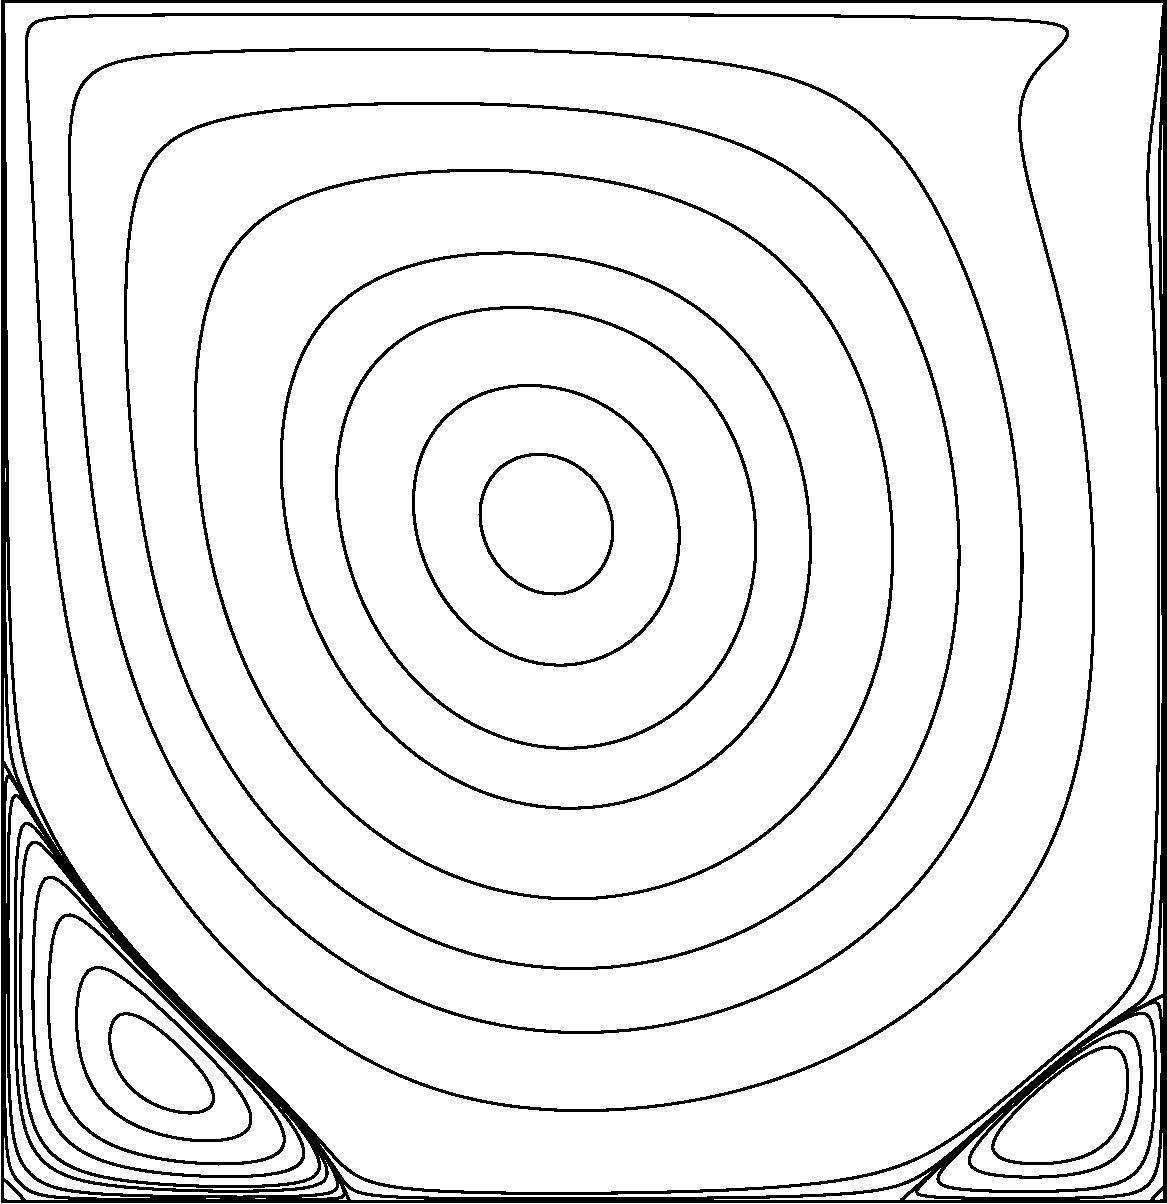
\includegraphics[width=0.85\textwidth]{Images/streamFunction.pdf}
    \caption{Stream function for $N = 64$, $\text{Re} = 1000$, $\Delta t = 0.0002$, and $\text{tol} = 1 \cdot 10^{-5}$.}
    \label{fig:SFN64}
\end{figure}

\begin{figure}[p]
    \centering
    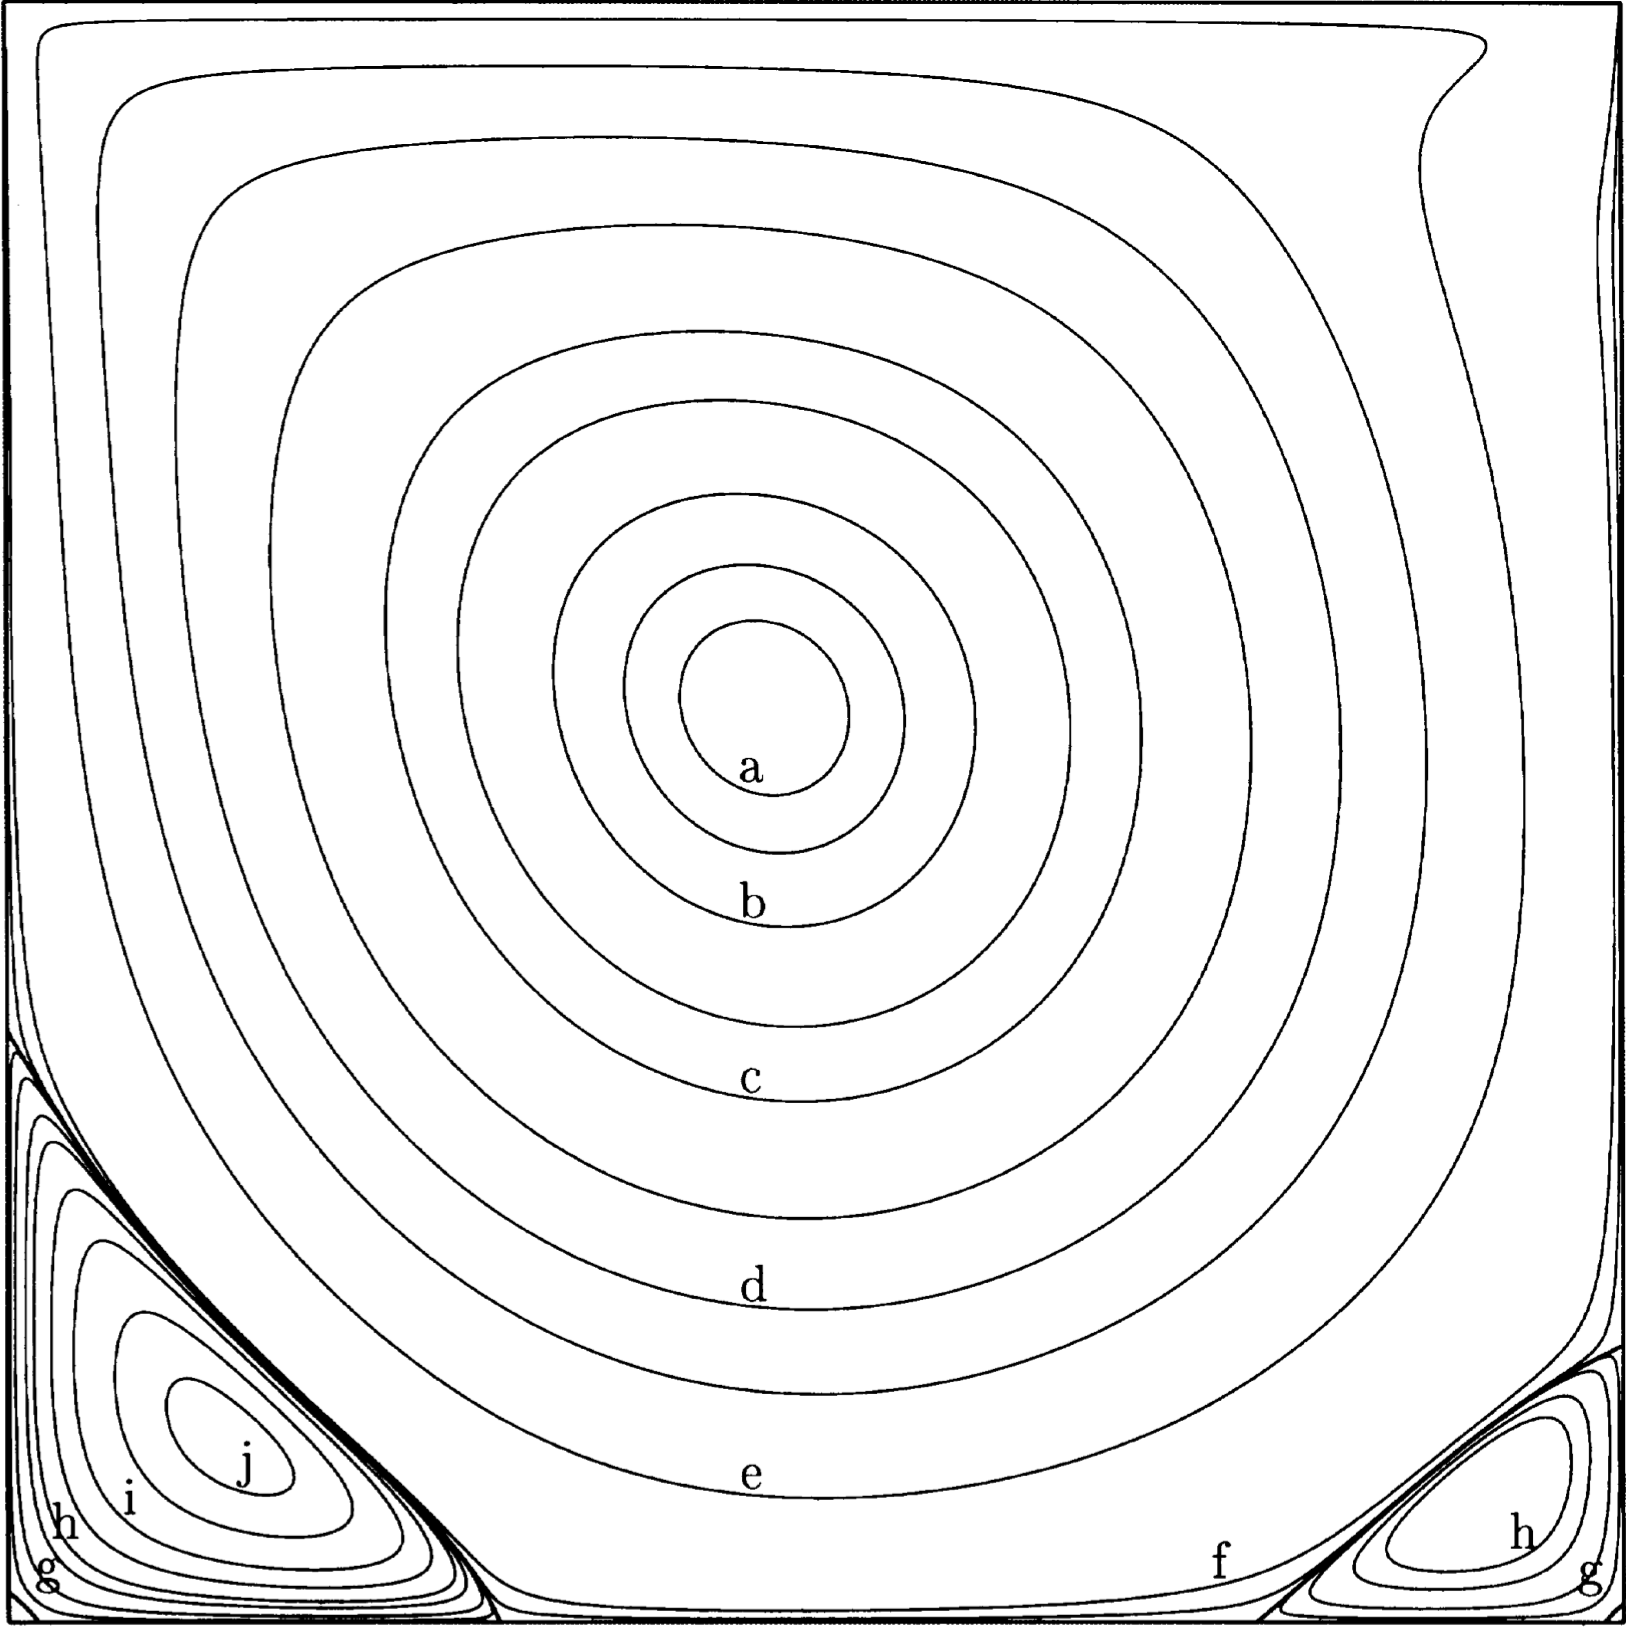
\includegraphics[width=0.85\textwidth]{Images/streamFunction.png}
    \caption{Benchmark stream function for $\text{Re} = 1000$ \parencite{botella1998benchmark}.}
    \label{fig:benchmarkSFN64}
\end{figure}

\begin{figure}[p]
    \centering
    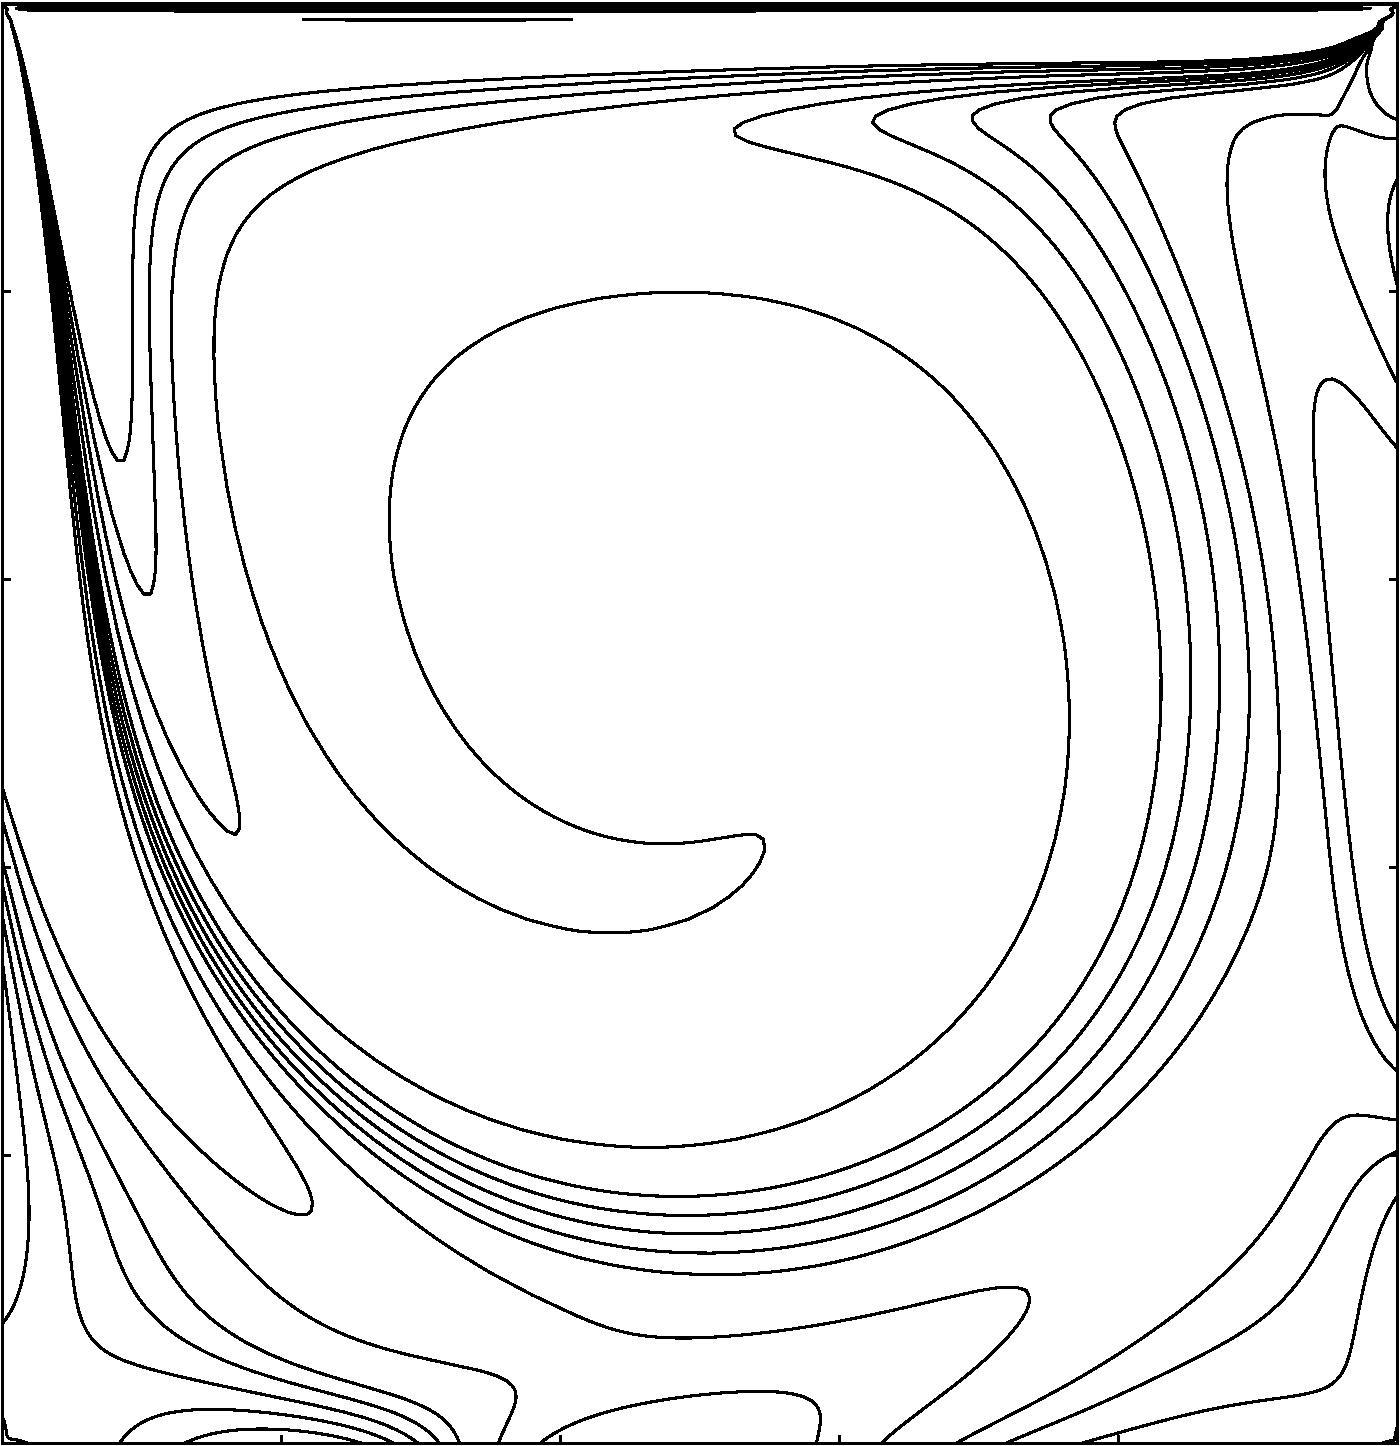
\includegraphics[width=0.85\textwidth]{Images/vorticity.pdf}
    \caption{Vorticity for $N = 64$, $\text{Re} = 1000$, $\Delta t = 0.0002$, and $\text{tol} = 1 \cdot 10^{-5}$.}
    \label{fig:VN64}
\end{figure}

\begin{figure}[p]
    \centering
    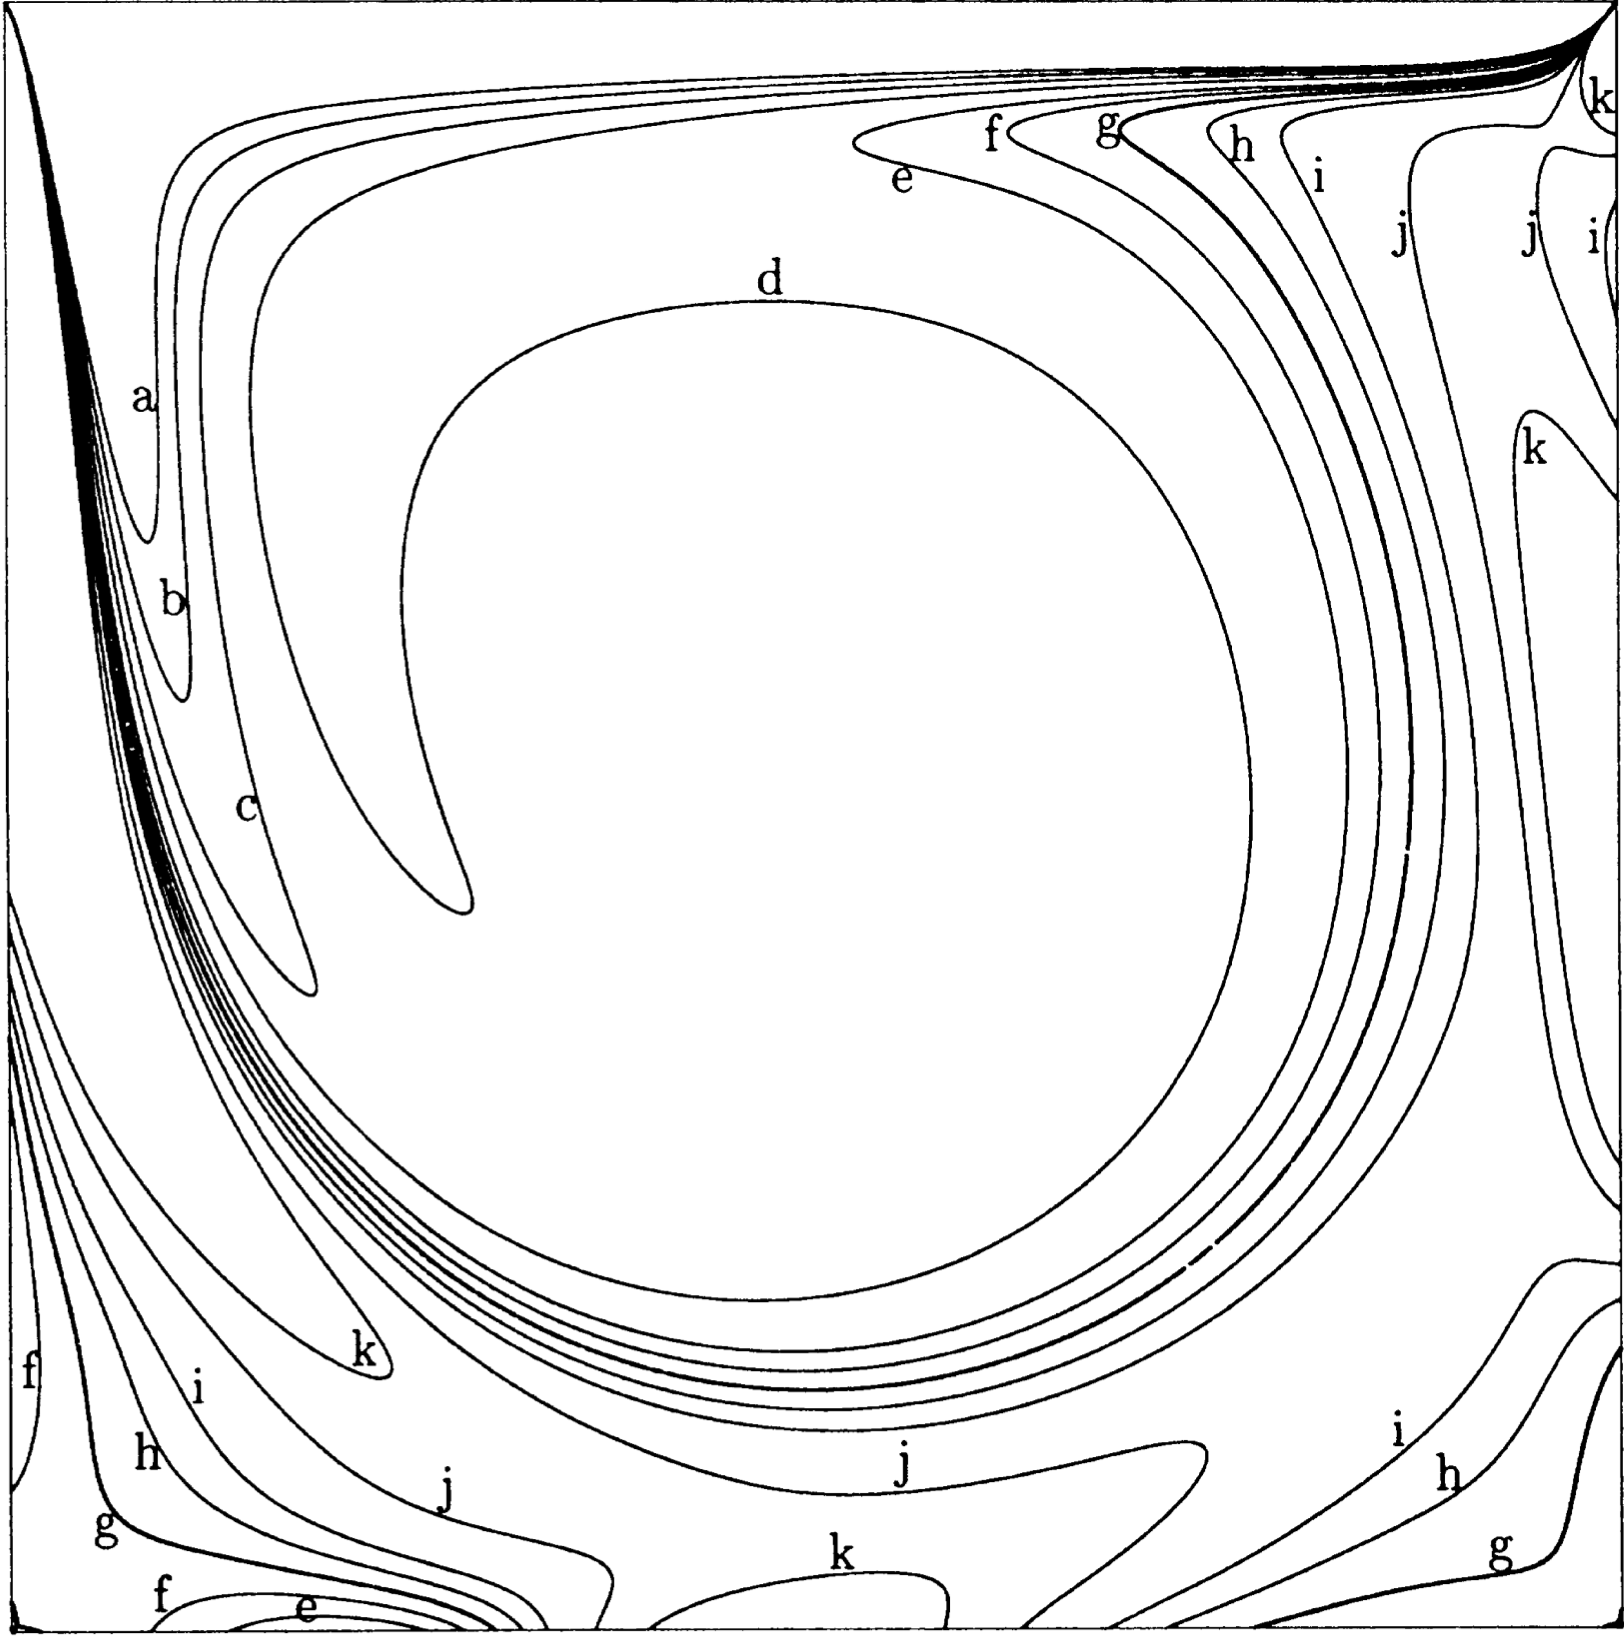
\includegraphics[width=0.85\textwidth]{Images/vorticity.png}
    \caption{Benchmark vorticity for $\text{Re} = 1000$ \parencite{botella1998benchmark}.}
    \label{fig:benchmarkVN64}
\end{figure}

\begin{figure}[p]
    \centering
    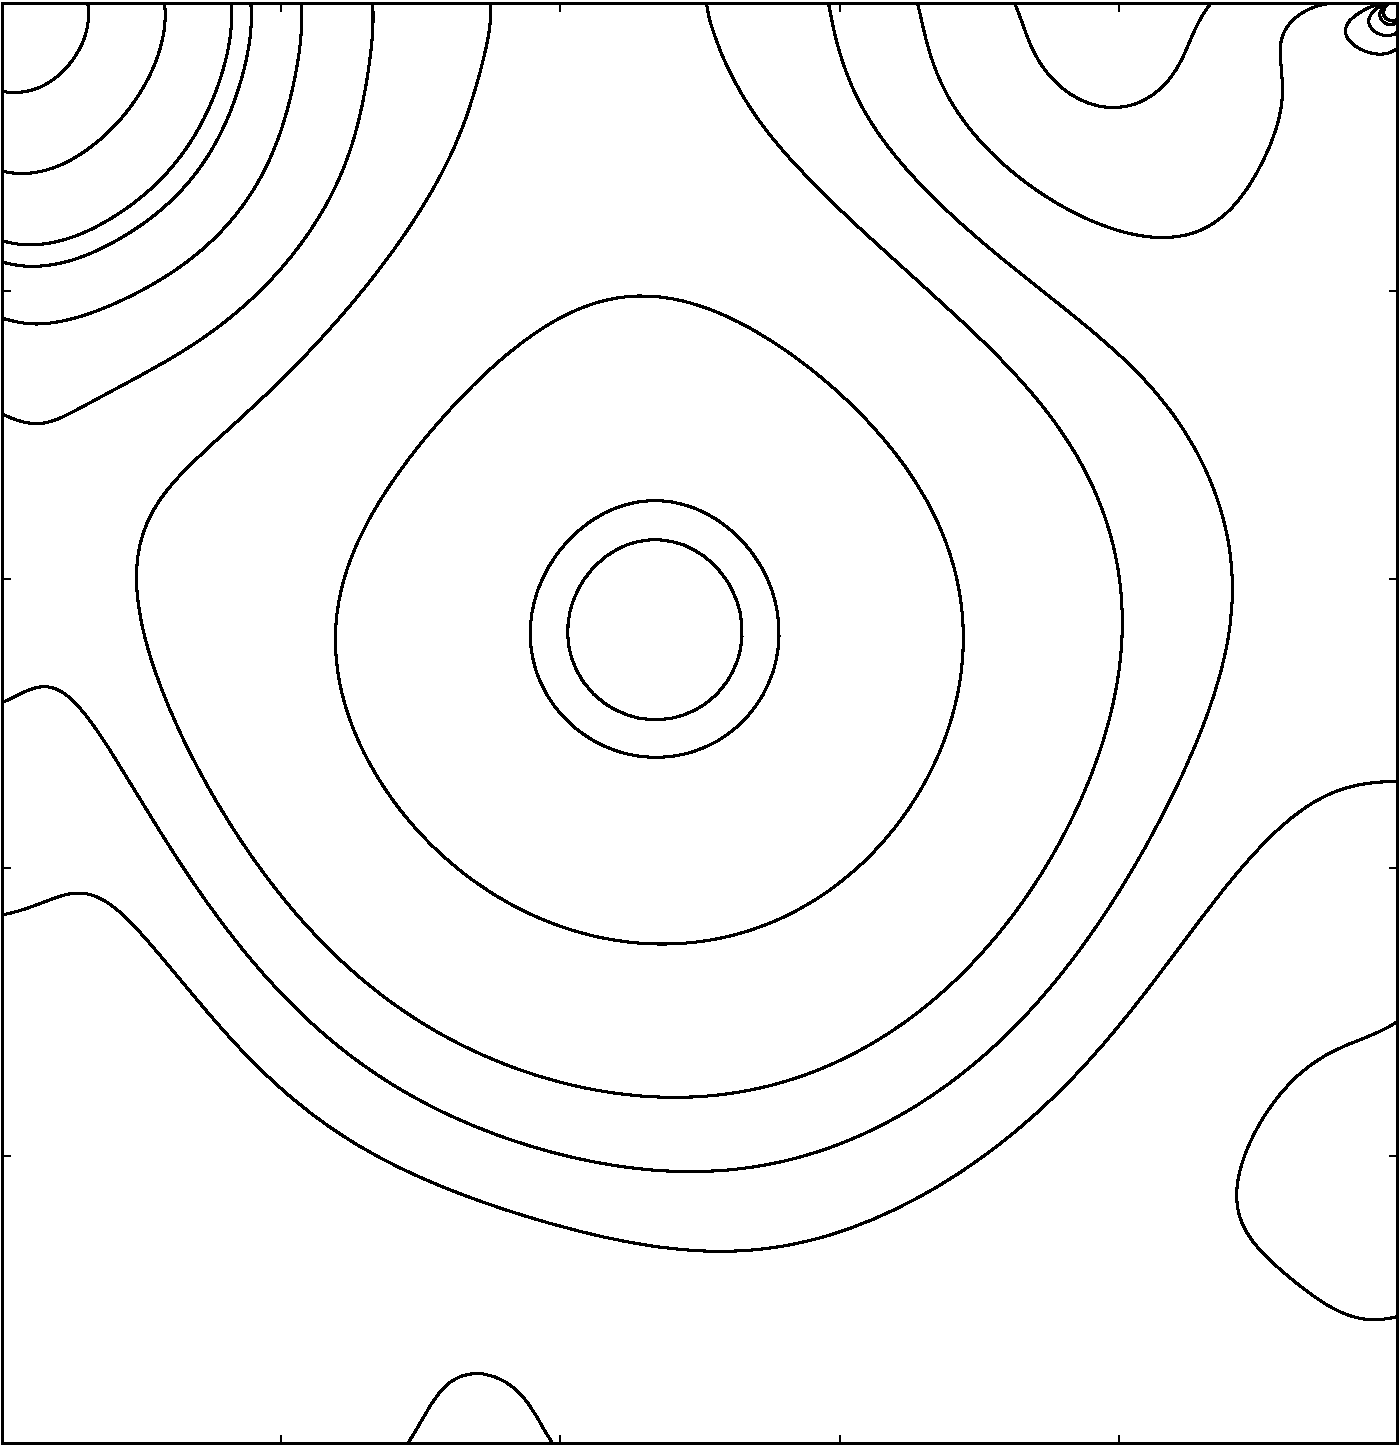
\includegraphics[width=0.85\textwidth]{Images/pressure.pdf}
    \caption{Pressure for $N = 64$, $\text{Re} = 1000$, $\Delta t = 0.0002$, and $\text{tol} = 1 \cdot 10^{-5}$.}
    \label{fig:PN64}
\end{figure}

\begin{figure}[p]
    \centering
    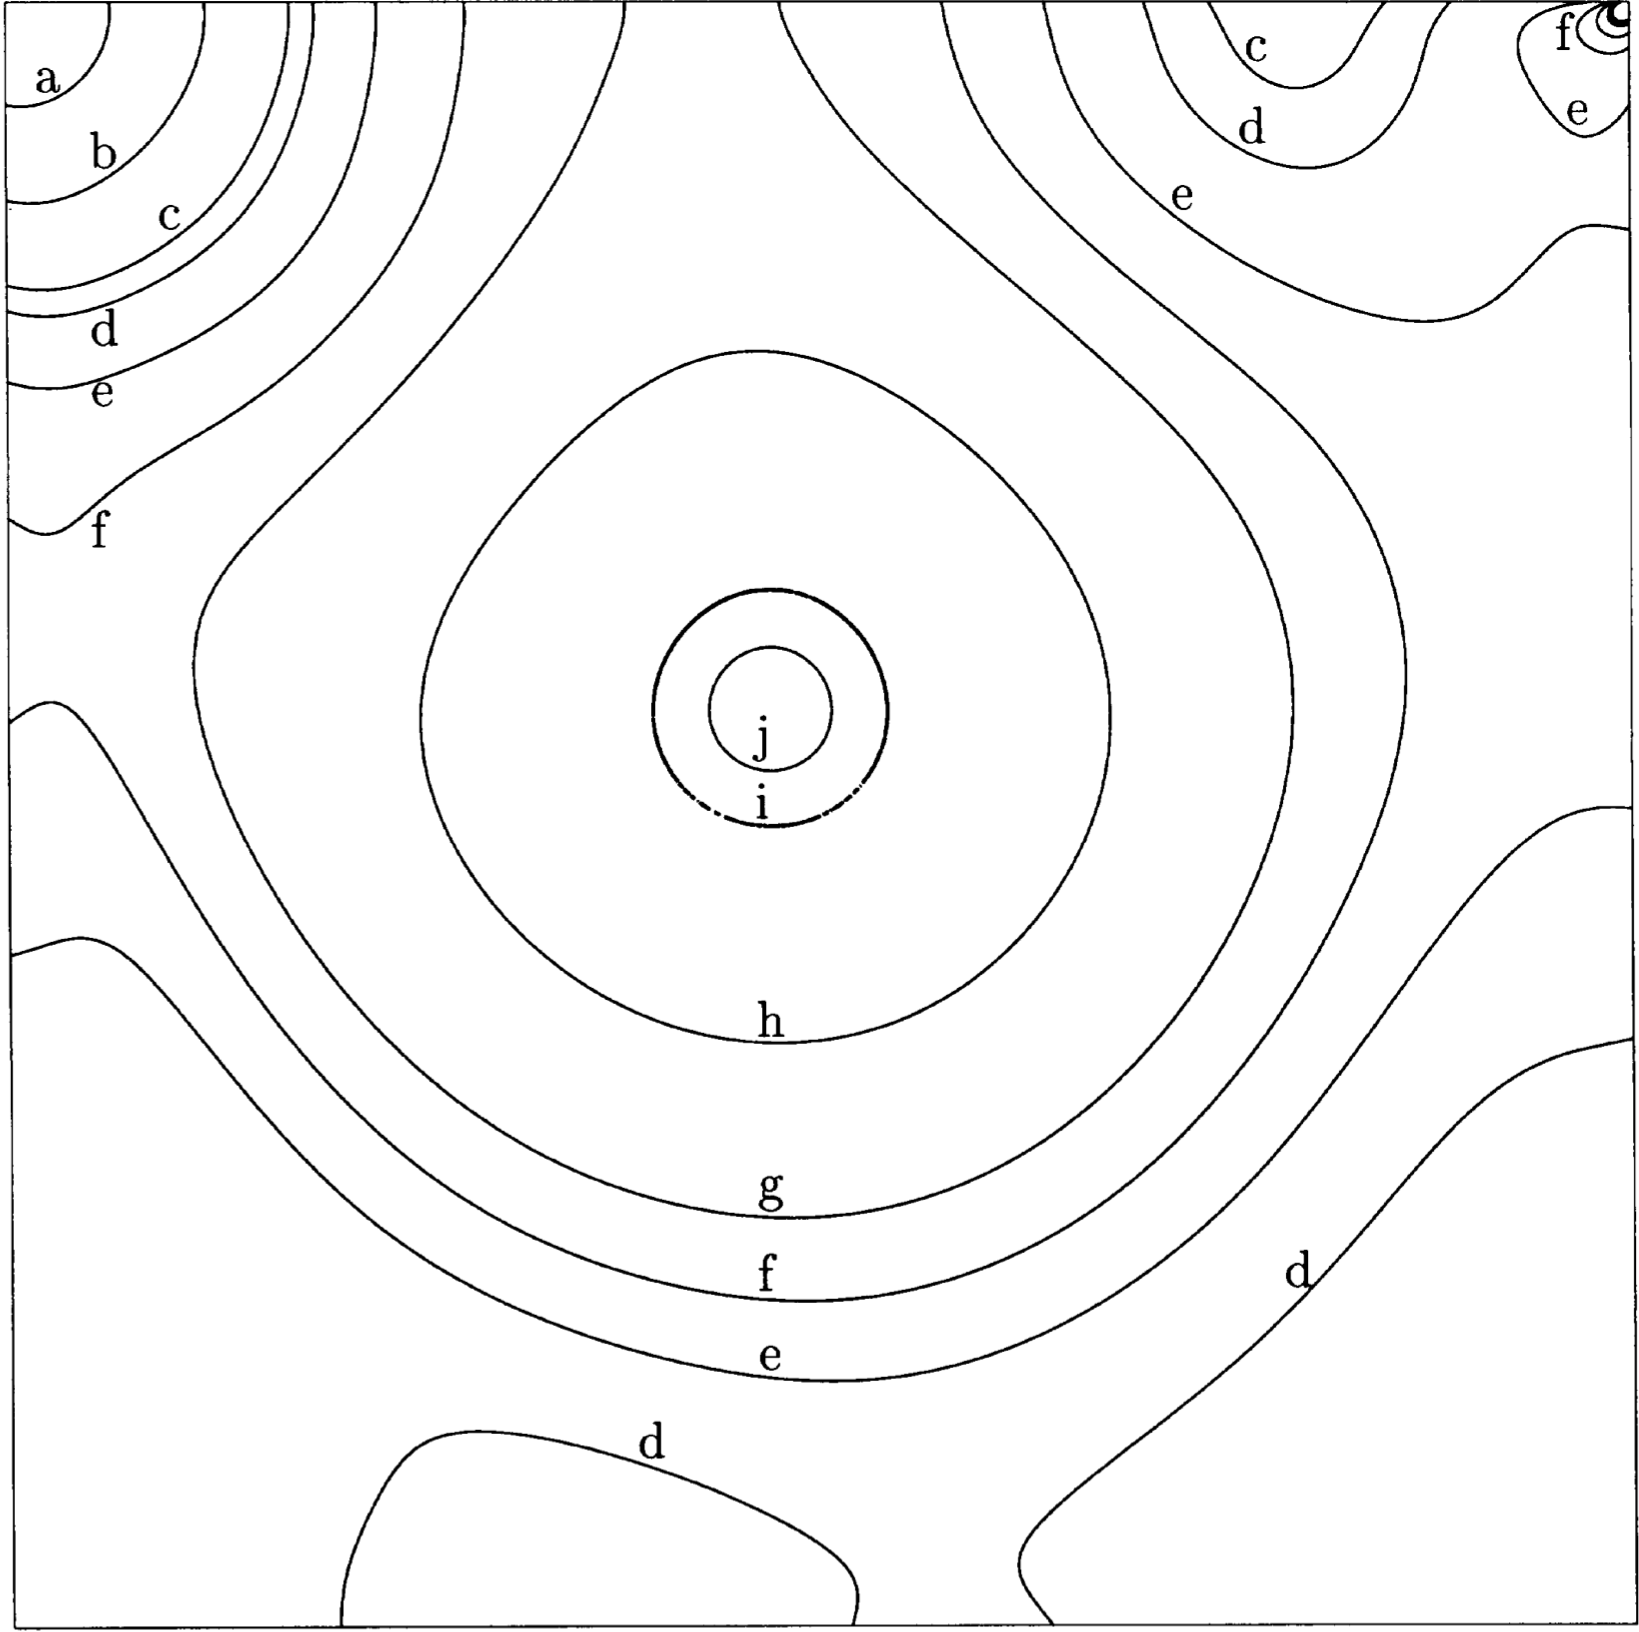
\includegraphics[width=0.85\textwidth]{Images/pressure.png}
    \caption{Benchmark pressure for $\text{Re} = 1000$ \parencite{botella1998benchmark}.}
    \label{fig:benchmarkPN64}
\end{figure}

\begin{figure}[p]
    \centering
    \begin{subfigure}[b]{0.49\textwidth}
        \centering{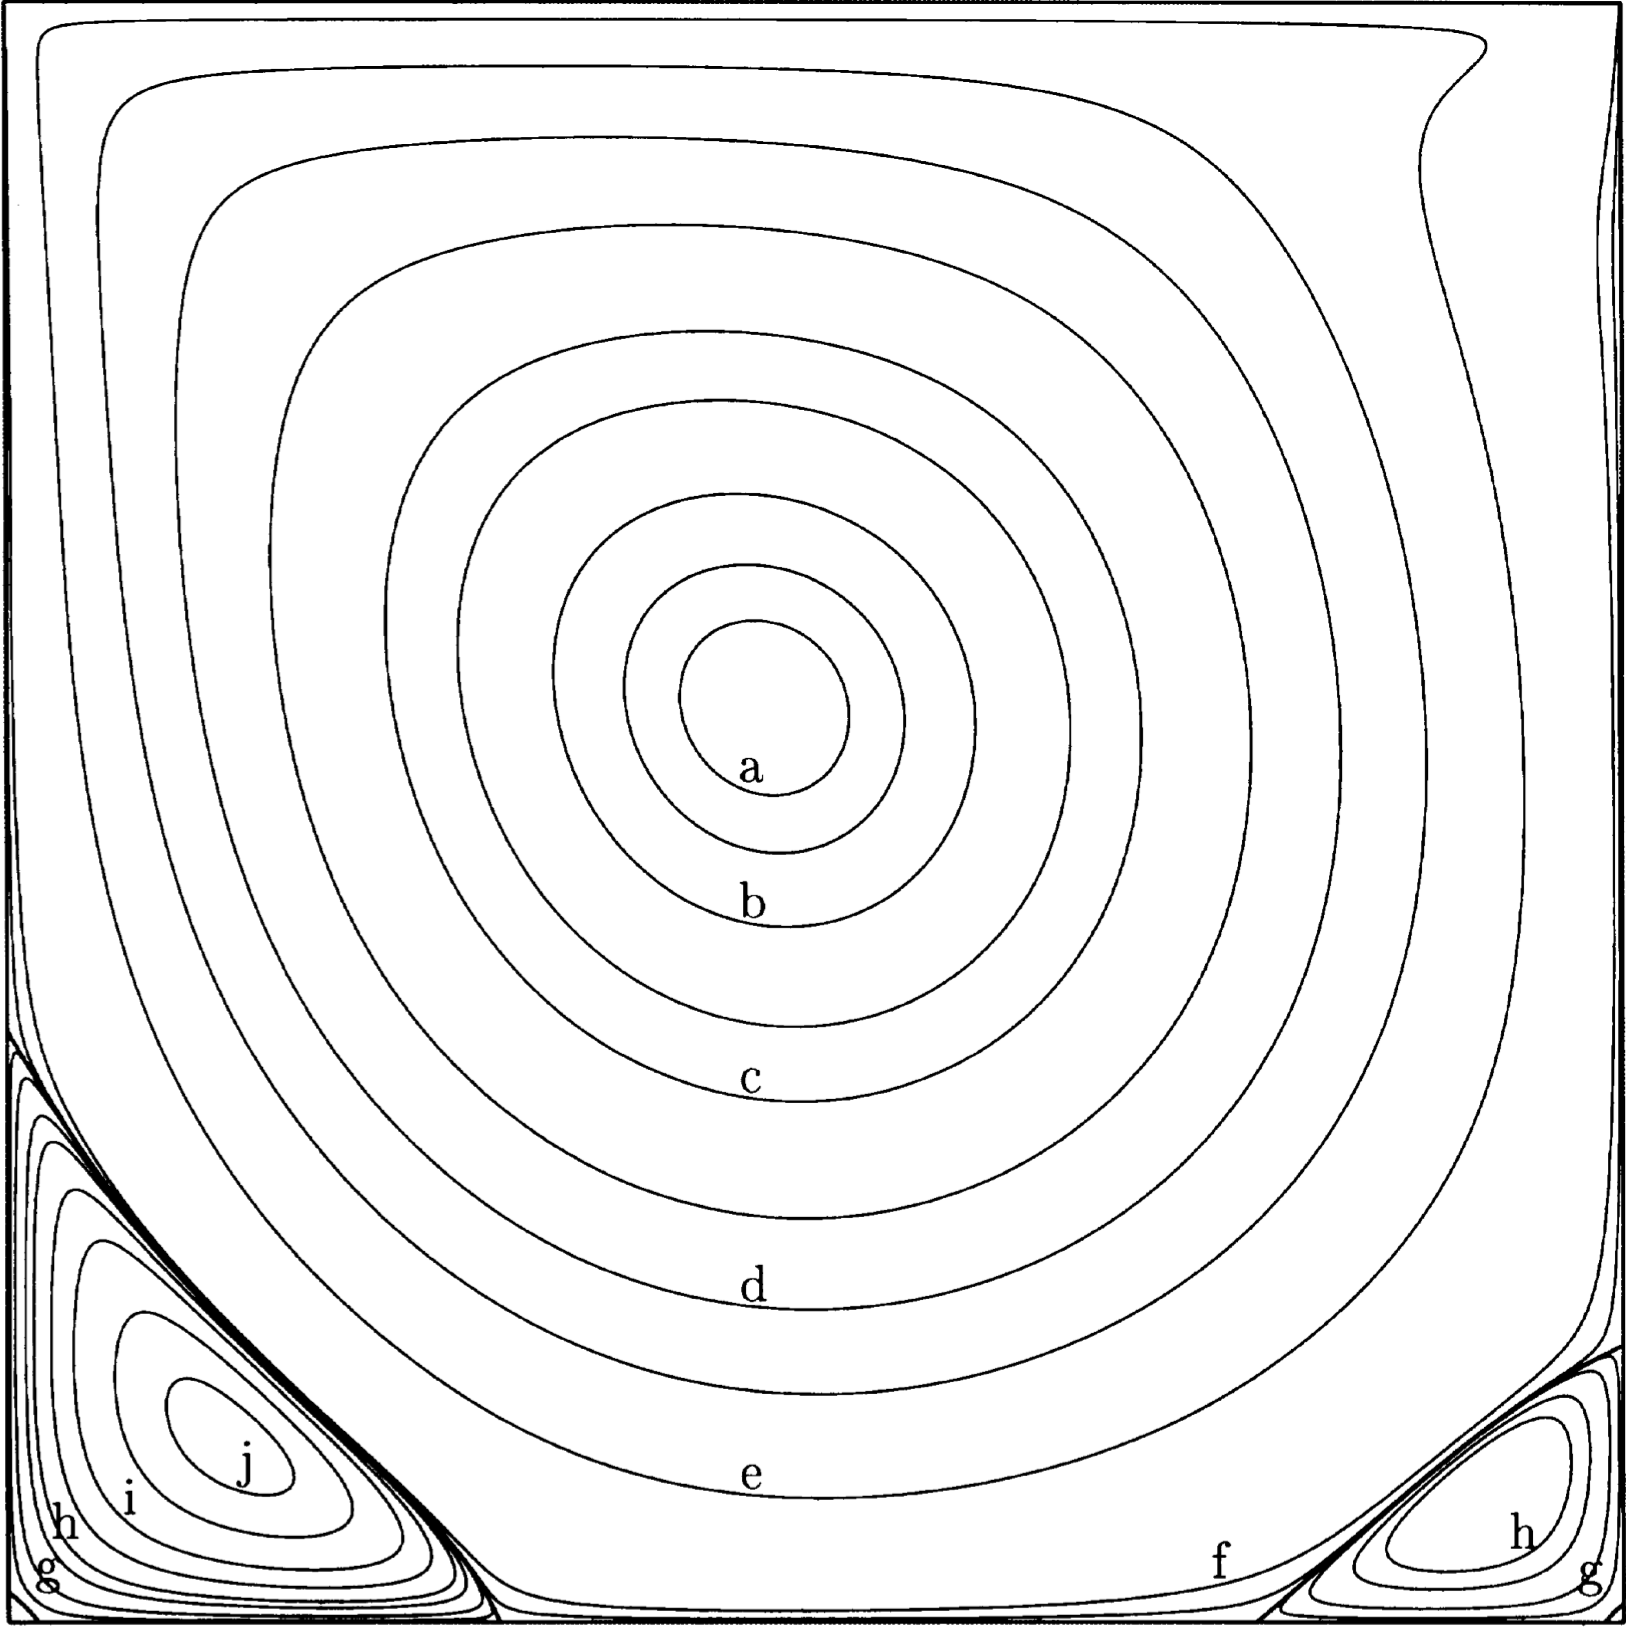
\includegraphics[width=0.95\linewidth]{Images/streamFunction.png}}
	    \caption{Benchmark}
    	\label{fig:sfa}
    \end{subfigure}
    % This comment avoids line break...
    \begin{subfigure}[b]{0.49\textwidth}
        \centering{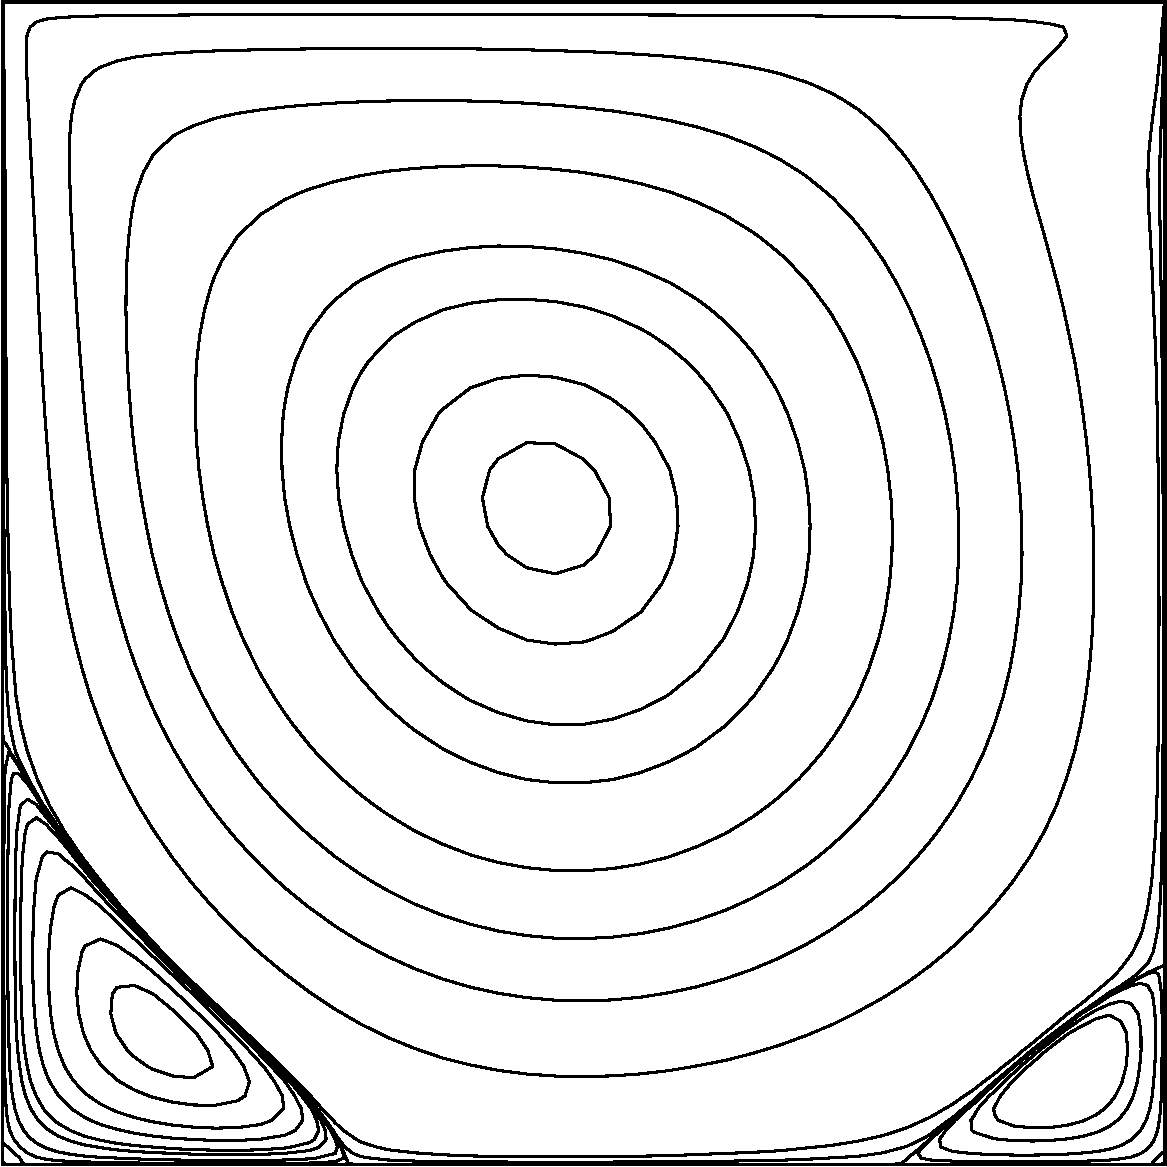
\includegraphics[width=0.95\linewidth]{Images/streamFunction64.pdf}}
	    \caption{$N = 64$}
    	\label{fig:sfb}
    \end{subfigure}
    
    \vspace{1cm}
    
    \begin{subfigure}[b]{0.49\textwidth}
        \centering{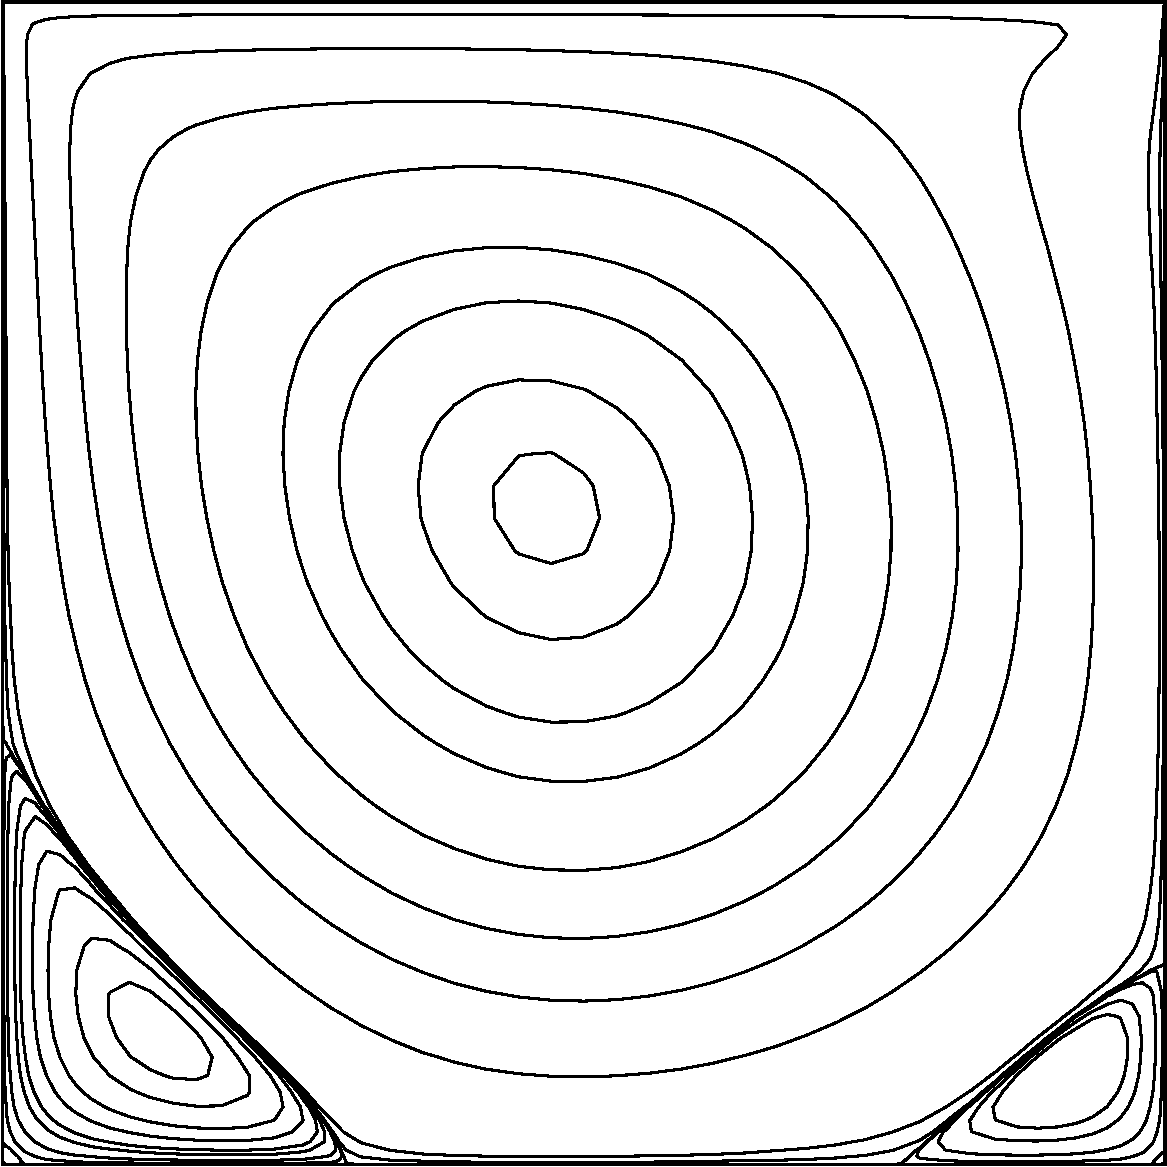
\includegraphics[width=0.95\linewidth]{Images/streamFunction56.pdf}}
	    \caption{$N = 56$}
    	\label{fig:sfc}
    \end{subfigure}
    % This comment avoids line break...
    \begin{subfigure}[b]{0.49\textwidth}
        \centering{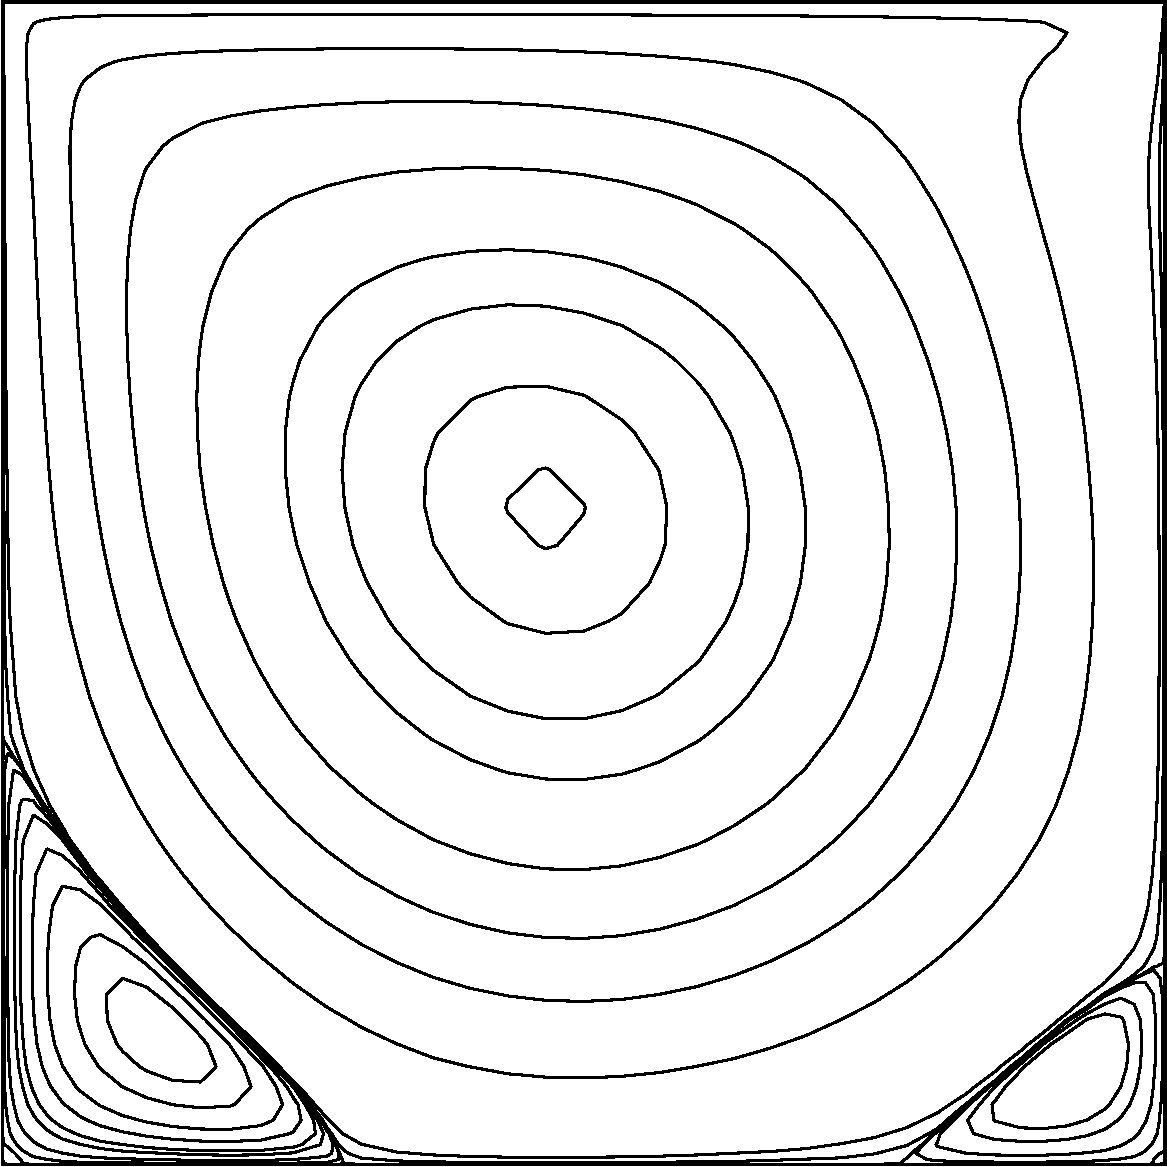
\includegraphics[width=0.95\linewidth]{Images/streamFunction48.pdf}}
	    \caption{$N = 48$}
    	\label{fig:sfd}
    \end{subfigure}
    
    \vspace{1cm}
    
    \begin{subfigure}[b]{0.49\textwidth}
        \centering{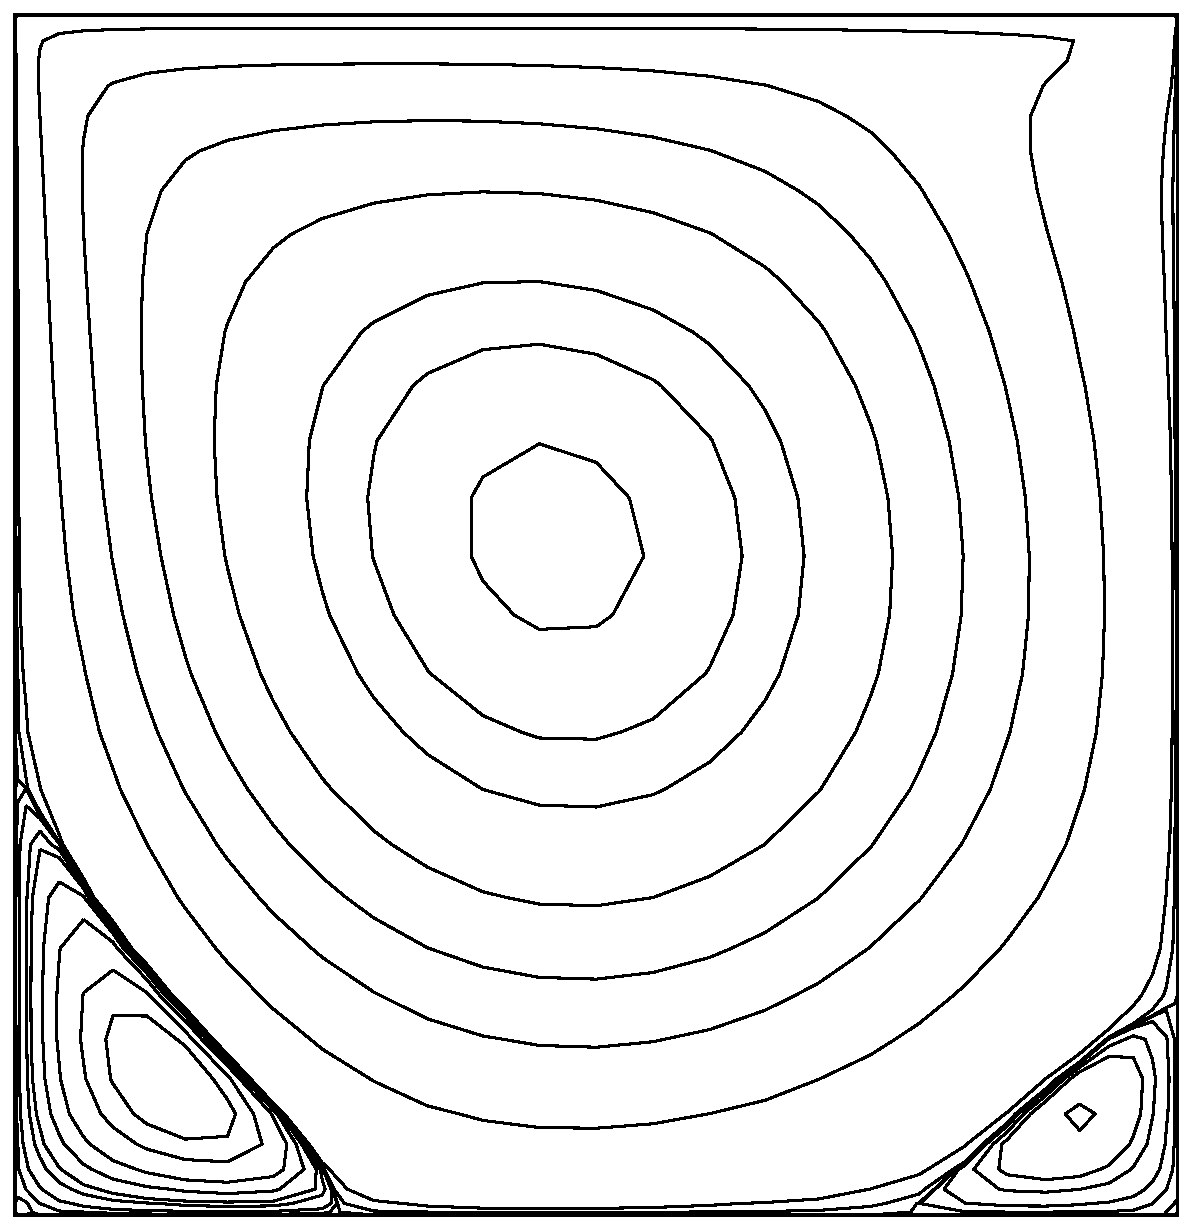
\includegraphics[width=0.95\linewidth]{Images/streamFunction32.pdf}}
	    \caption{$N = 32$}
    	\label{fig:sfe}
    \end{subfigure}
    % This comment avoids line break...
    \begin{subfigure}[b]{0.49\textwidth}
        \centering{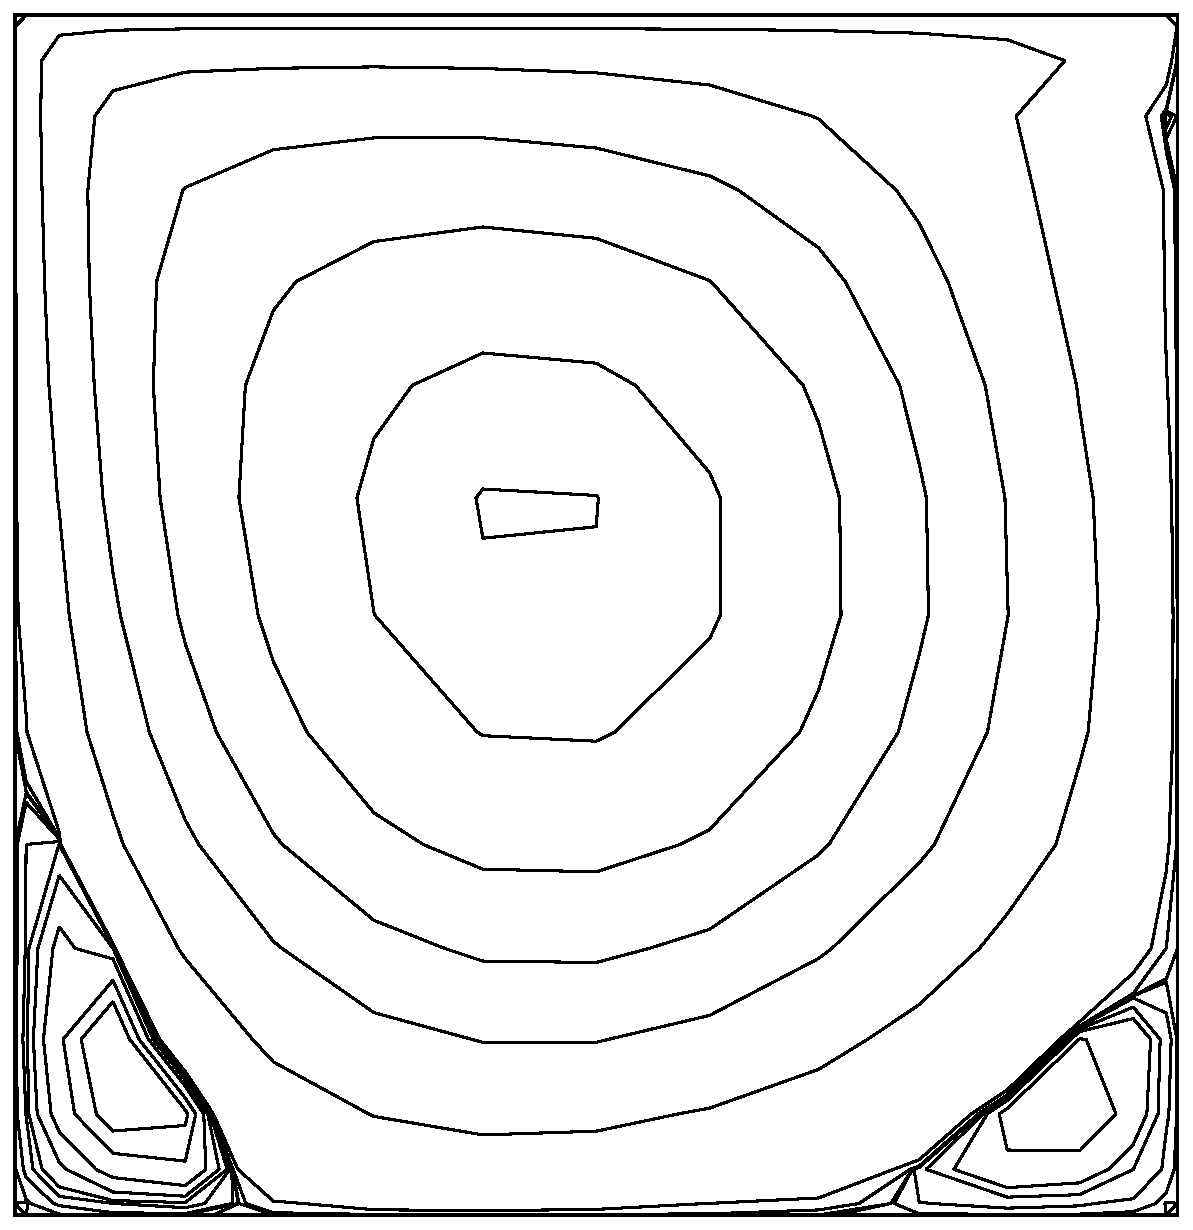
\includegraphics[width=0.95\linewidth]{Images/streamFunction16.pdf}}
	    \caption{$N = 16$}
    	\label{fig:sff}
    \end{subfigure}
    \caption{Stream function for $\text{Re} = 1000$, $\Delta t = 0.0002$, $\text{tol} = 1 \cdot 10^{-5}$, and various values of $N$ as well as the benchmark result}
    \label{fig:allsf}
\end{figure}

\begin{figure}[p]
    \centering
    \begin{subfigure}[b]{0.49\textwidth}
        \centering{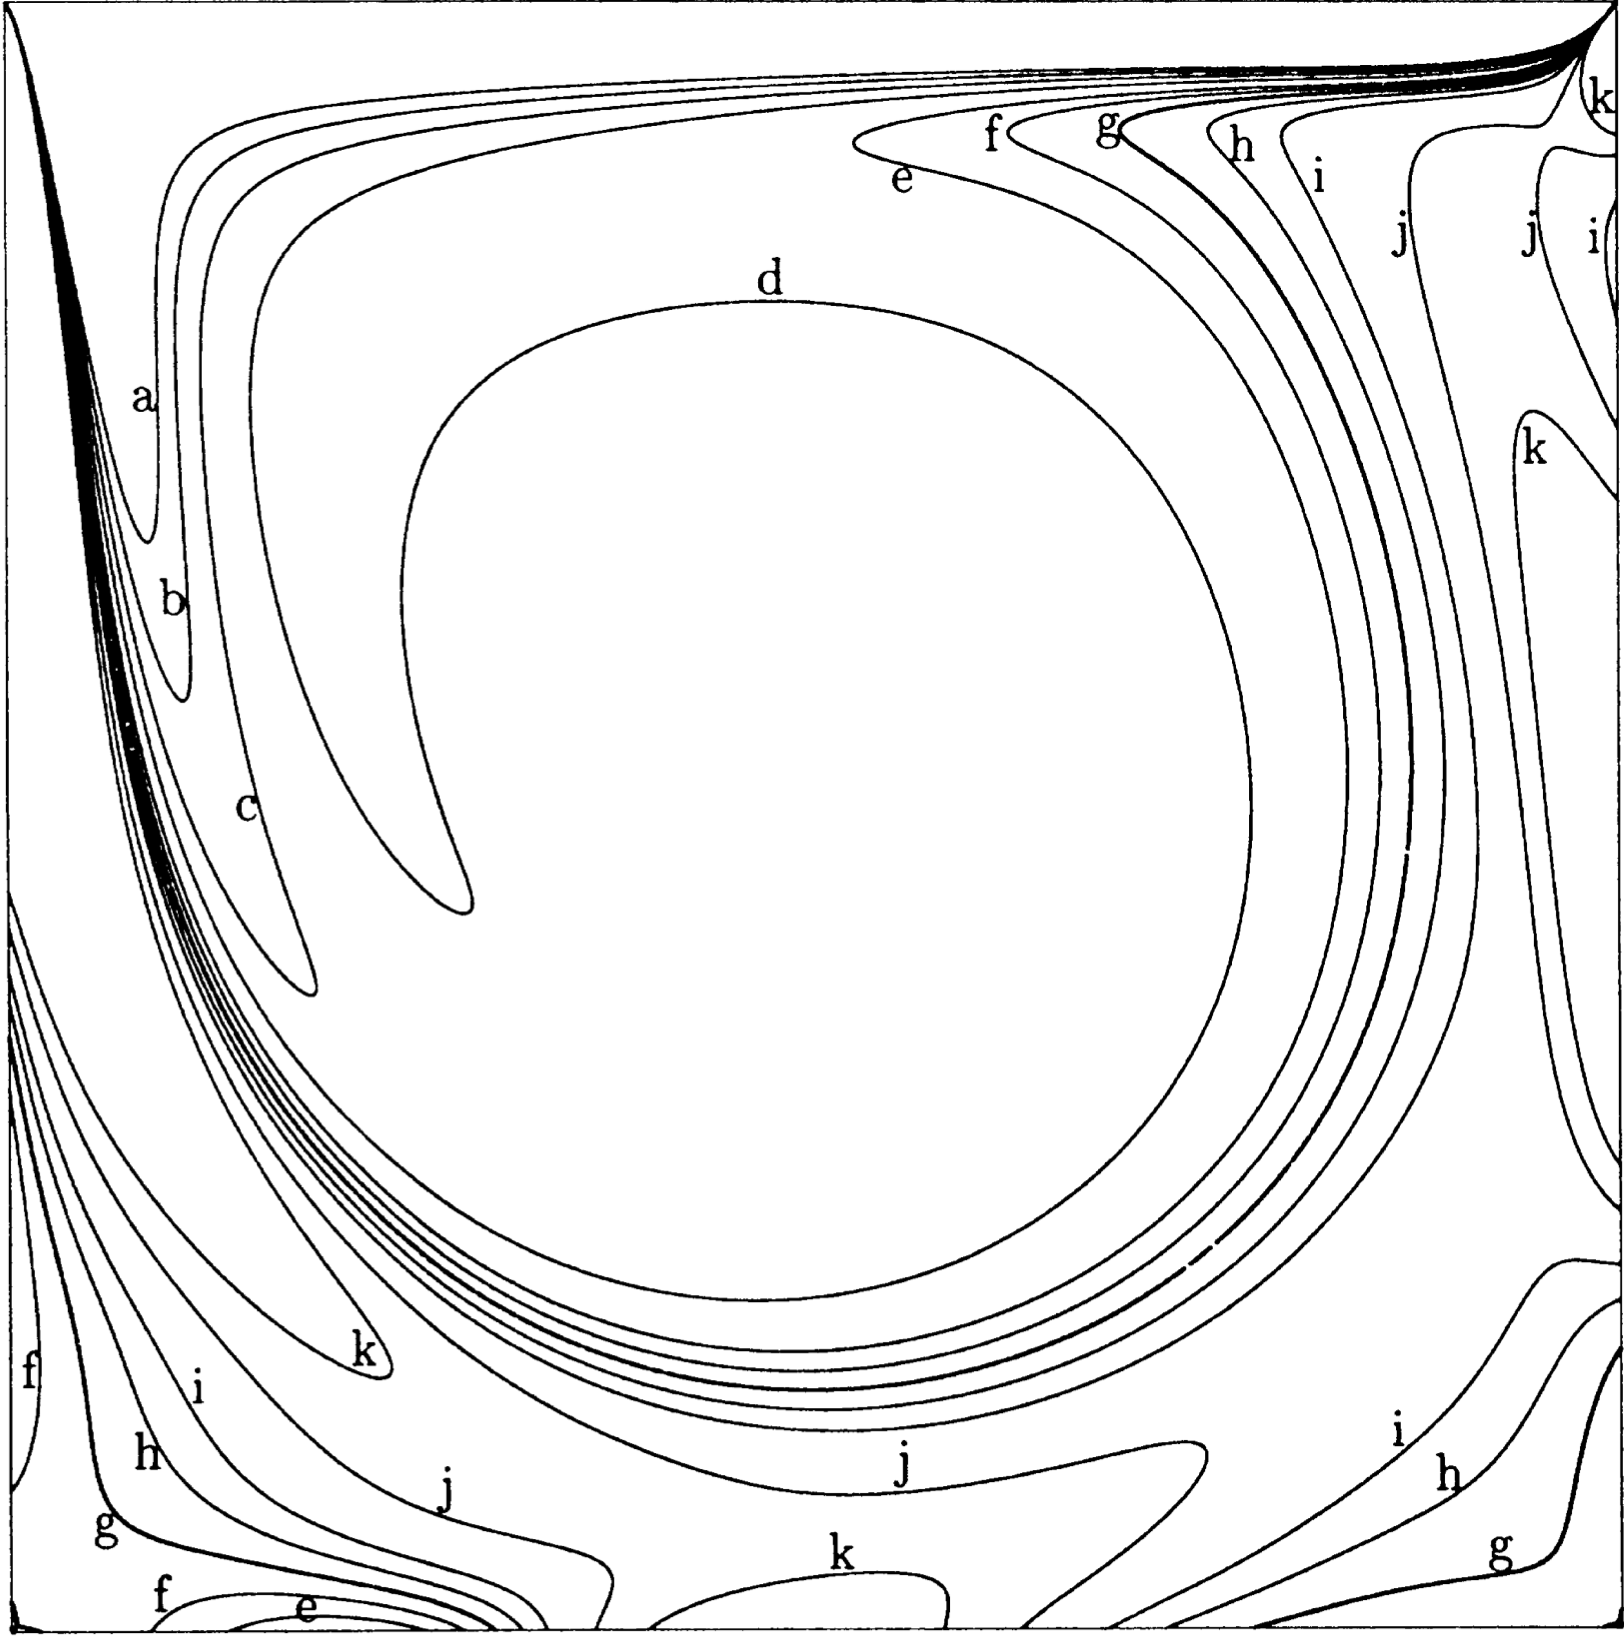
\includegraphics[width=0.95\linewidth]{Images/vorticity.png}}
	    \caption{Benchmark}
    	\label{fig:va}
    \end{subfigure}
    % This comment avoids line break...
    \begin{subfigure}[b]{0.49\textwidth}
        \centering{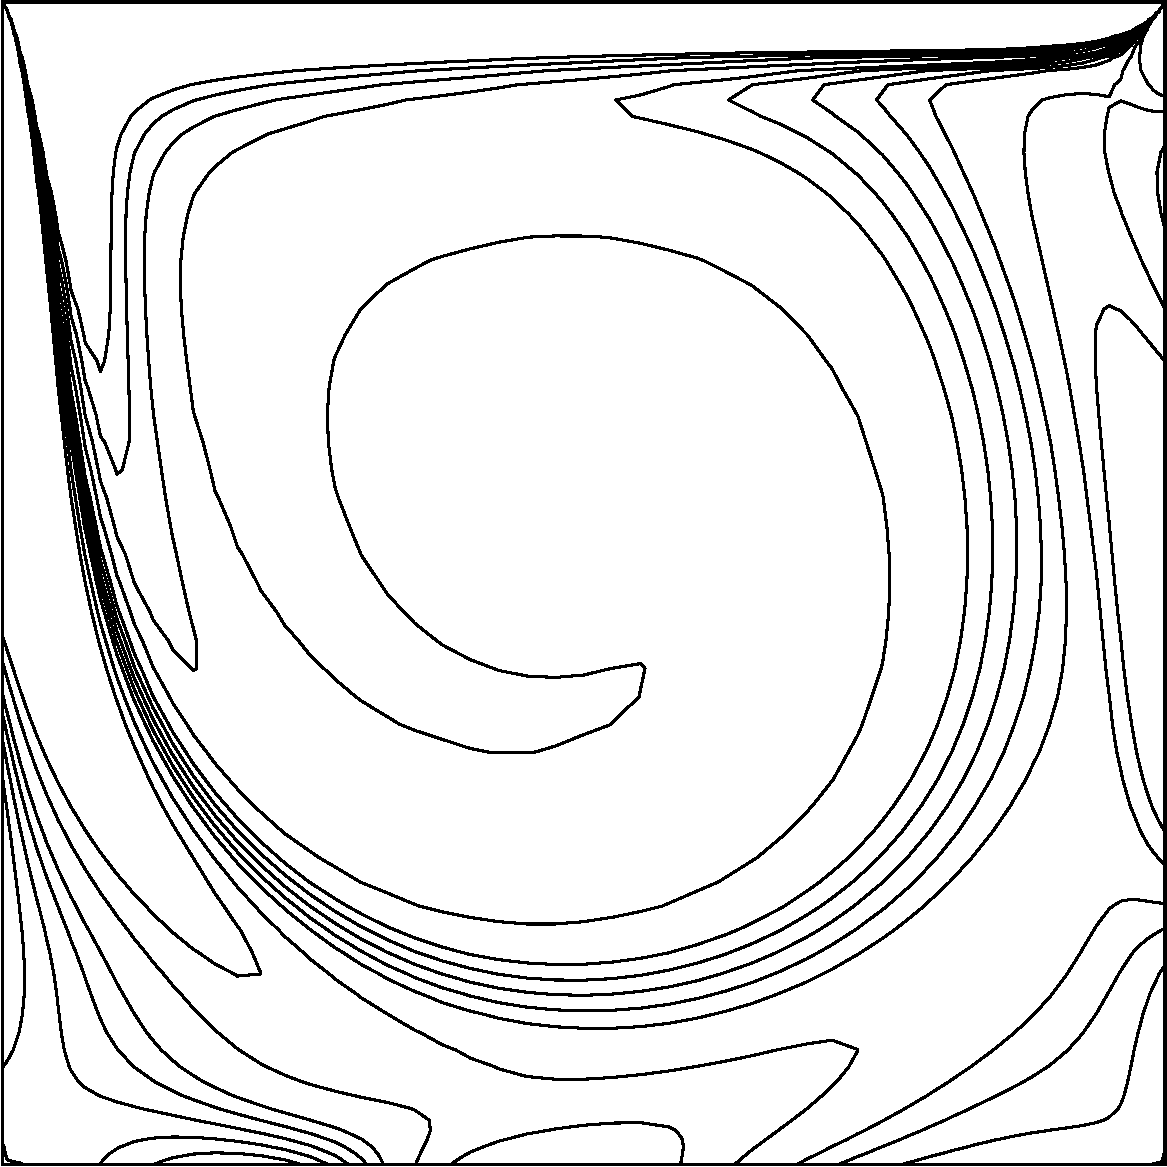
\includegraphics[width=0.95\linewidth]{Images/vorticity64.pdf}}
	    \caption{$N = 64$}
	    \label{fig:vb}	
    \end{subfigure}
    
    \vspace{1cm}
    
    \begin{subfigure}[b]{0.49\textwidth}
        \centering{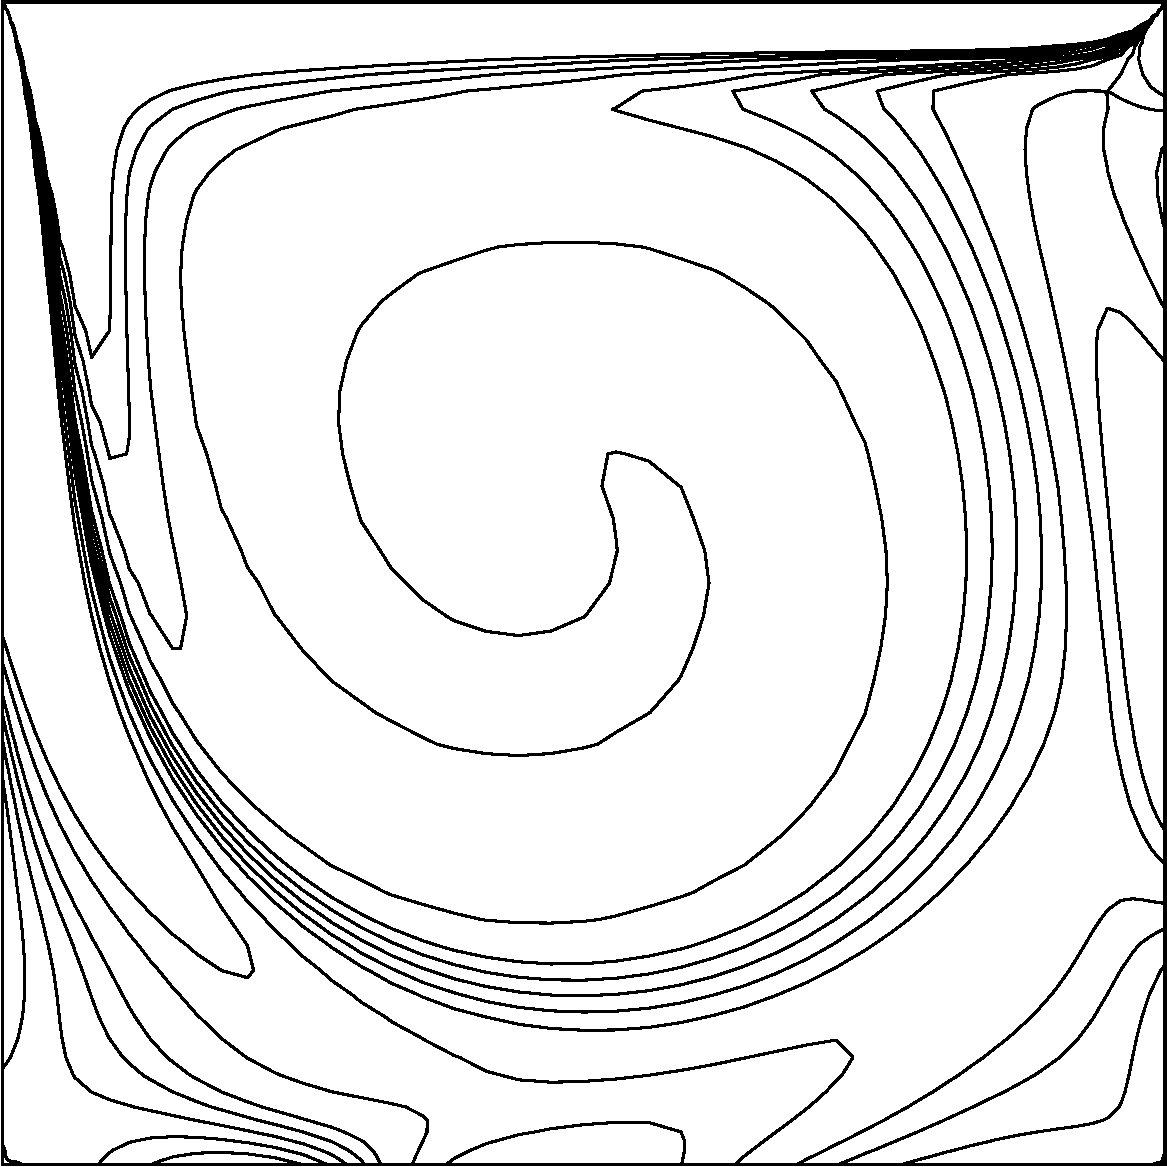
\includegraphics[width=0.95\linewidth]{Images/vorticity56.pdf}}
	    \caption{$N = 56$}
    	\label{fig:vc}
    \end{subfigure}
    % This comment avoids line break...
    \begin{subfigure}[b]{0.49\textwidth}
        \centering{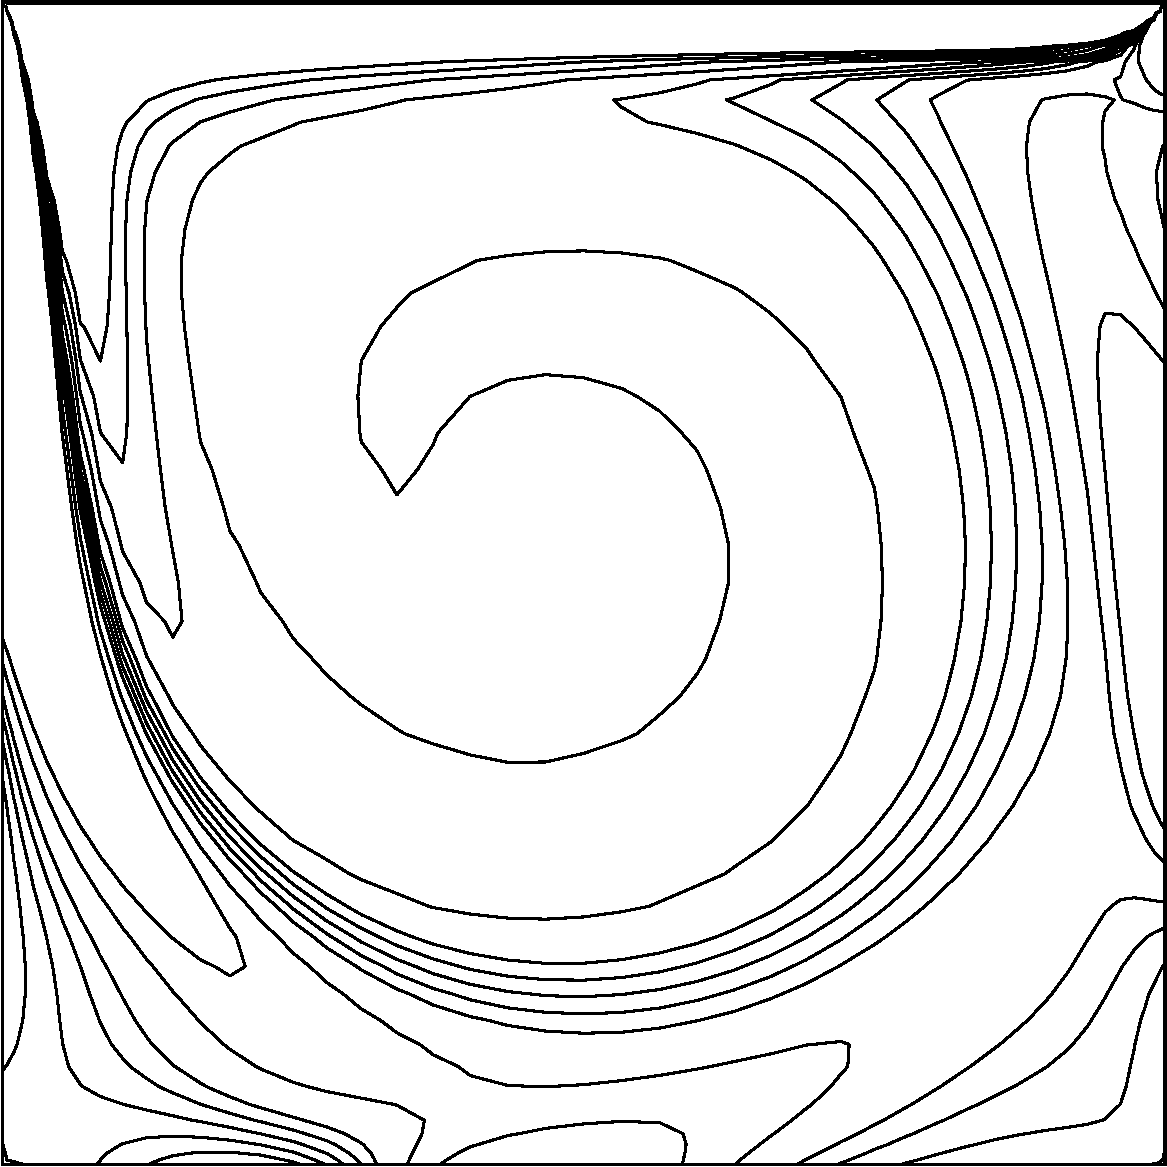
\includegraphics[width=0.95\linewidth]{Images/vorticity48.pdf}}
	    \caption{$N = 48$}
	    \label{fig:vd}	
    \end{subfigure}
    
    \vspace{1cm}
    
    \begin{subfigure}[b]{0.49\textwidth}
        \centering{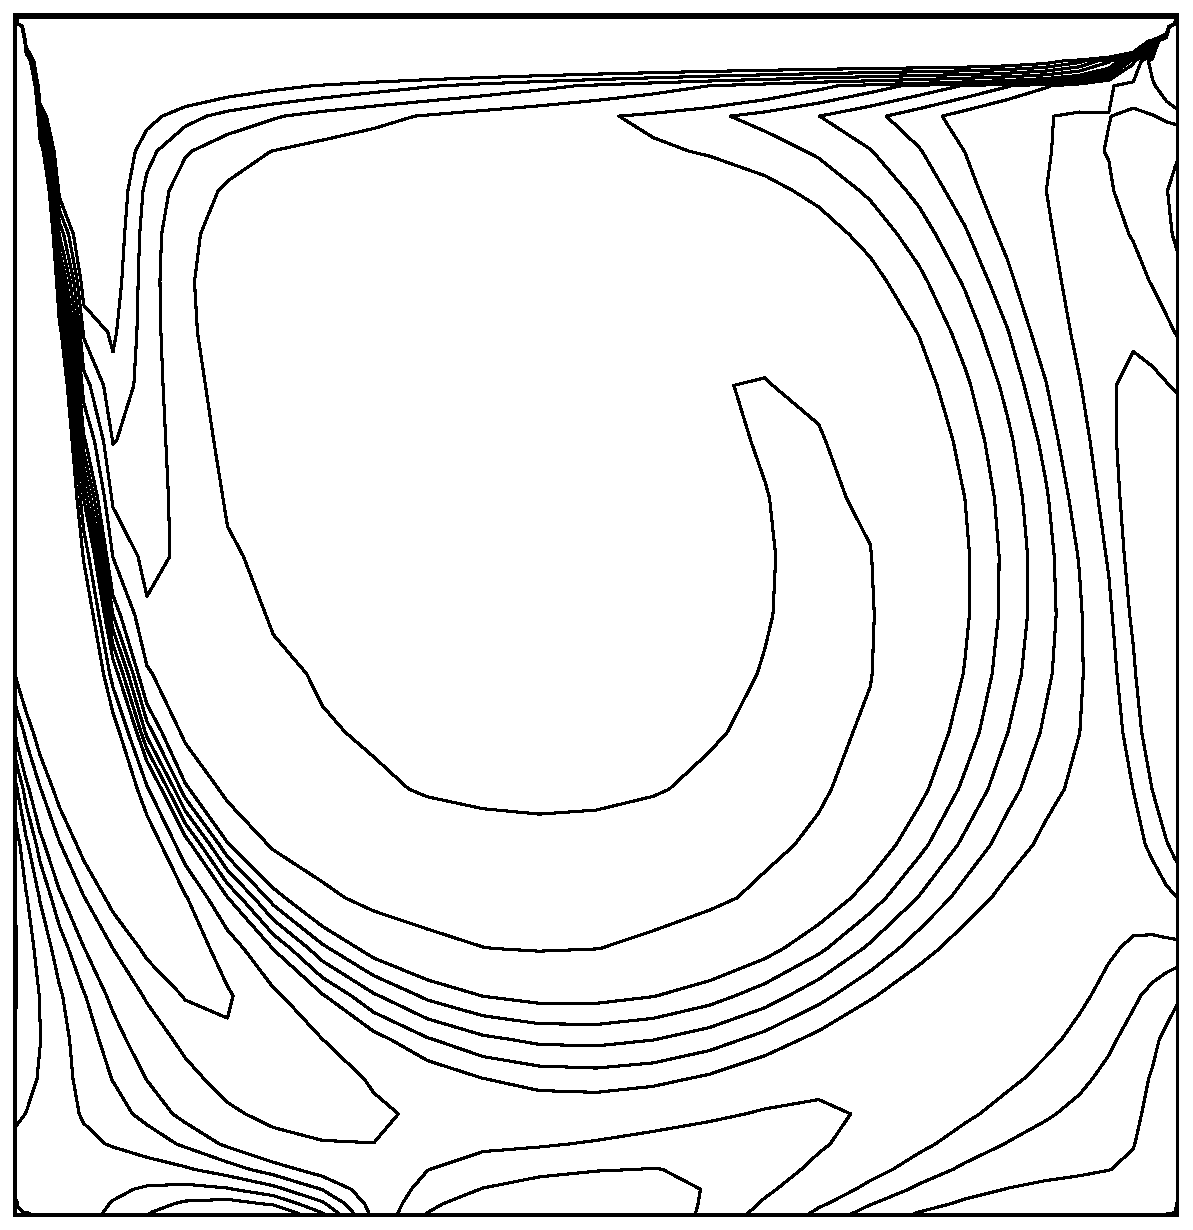
\includegraphics[width=0.95\linewidth]{Images/vorticity32.pdf}}
	    \caption{$N = 32$}
    	\label{fig:ve}
    \end{subfigure}
    % This comment avoids line break...
    \begin{subfigure}[b]{0.49\textwidth}
        \centering{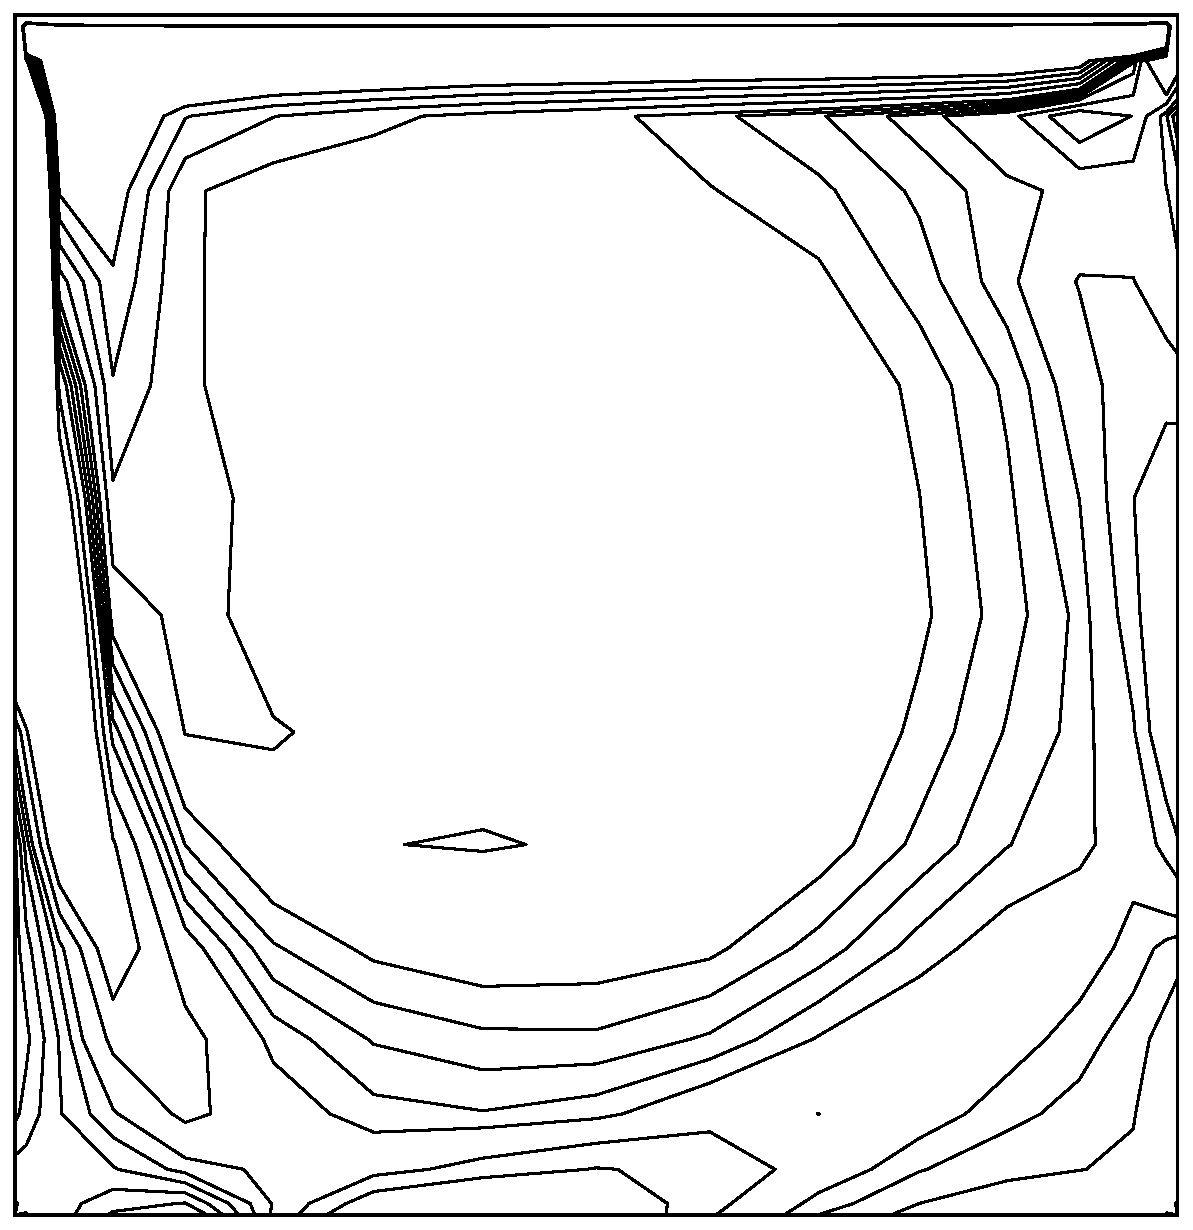
\includegraphics[width=0.95\linewidth]{Images/vorticity16.pdf}}
	    \caption{$N = 16$}
	    \label{fig:vf}
    \end{subfigure}
    \caption{Vorticity for $\text{Re} = 1000$, $\Delta t = 0.0002$, $\text{tol} = 1 \cdot 10^{-5}$, and various values of $N$ as well as the benchmark result.}
    \label{fig:allvorticity}
\end{figure}

\begin{figure}[p]
    \centering
    \begin{subfigure}[b]{0.49\textwidth}
        \centering{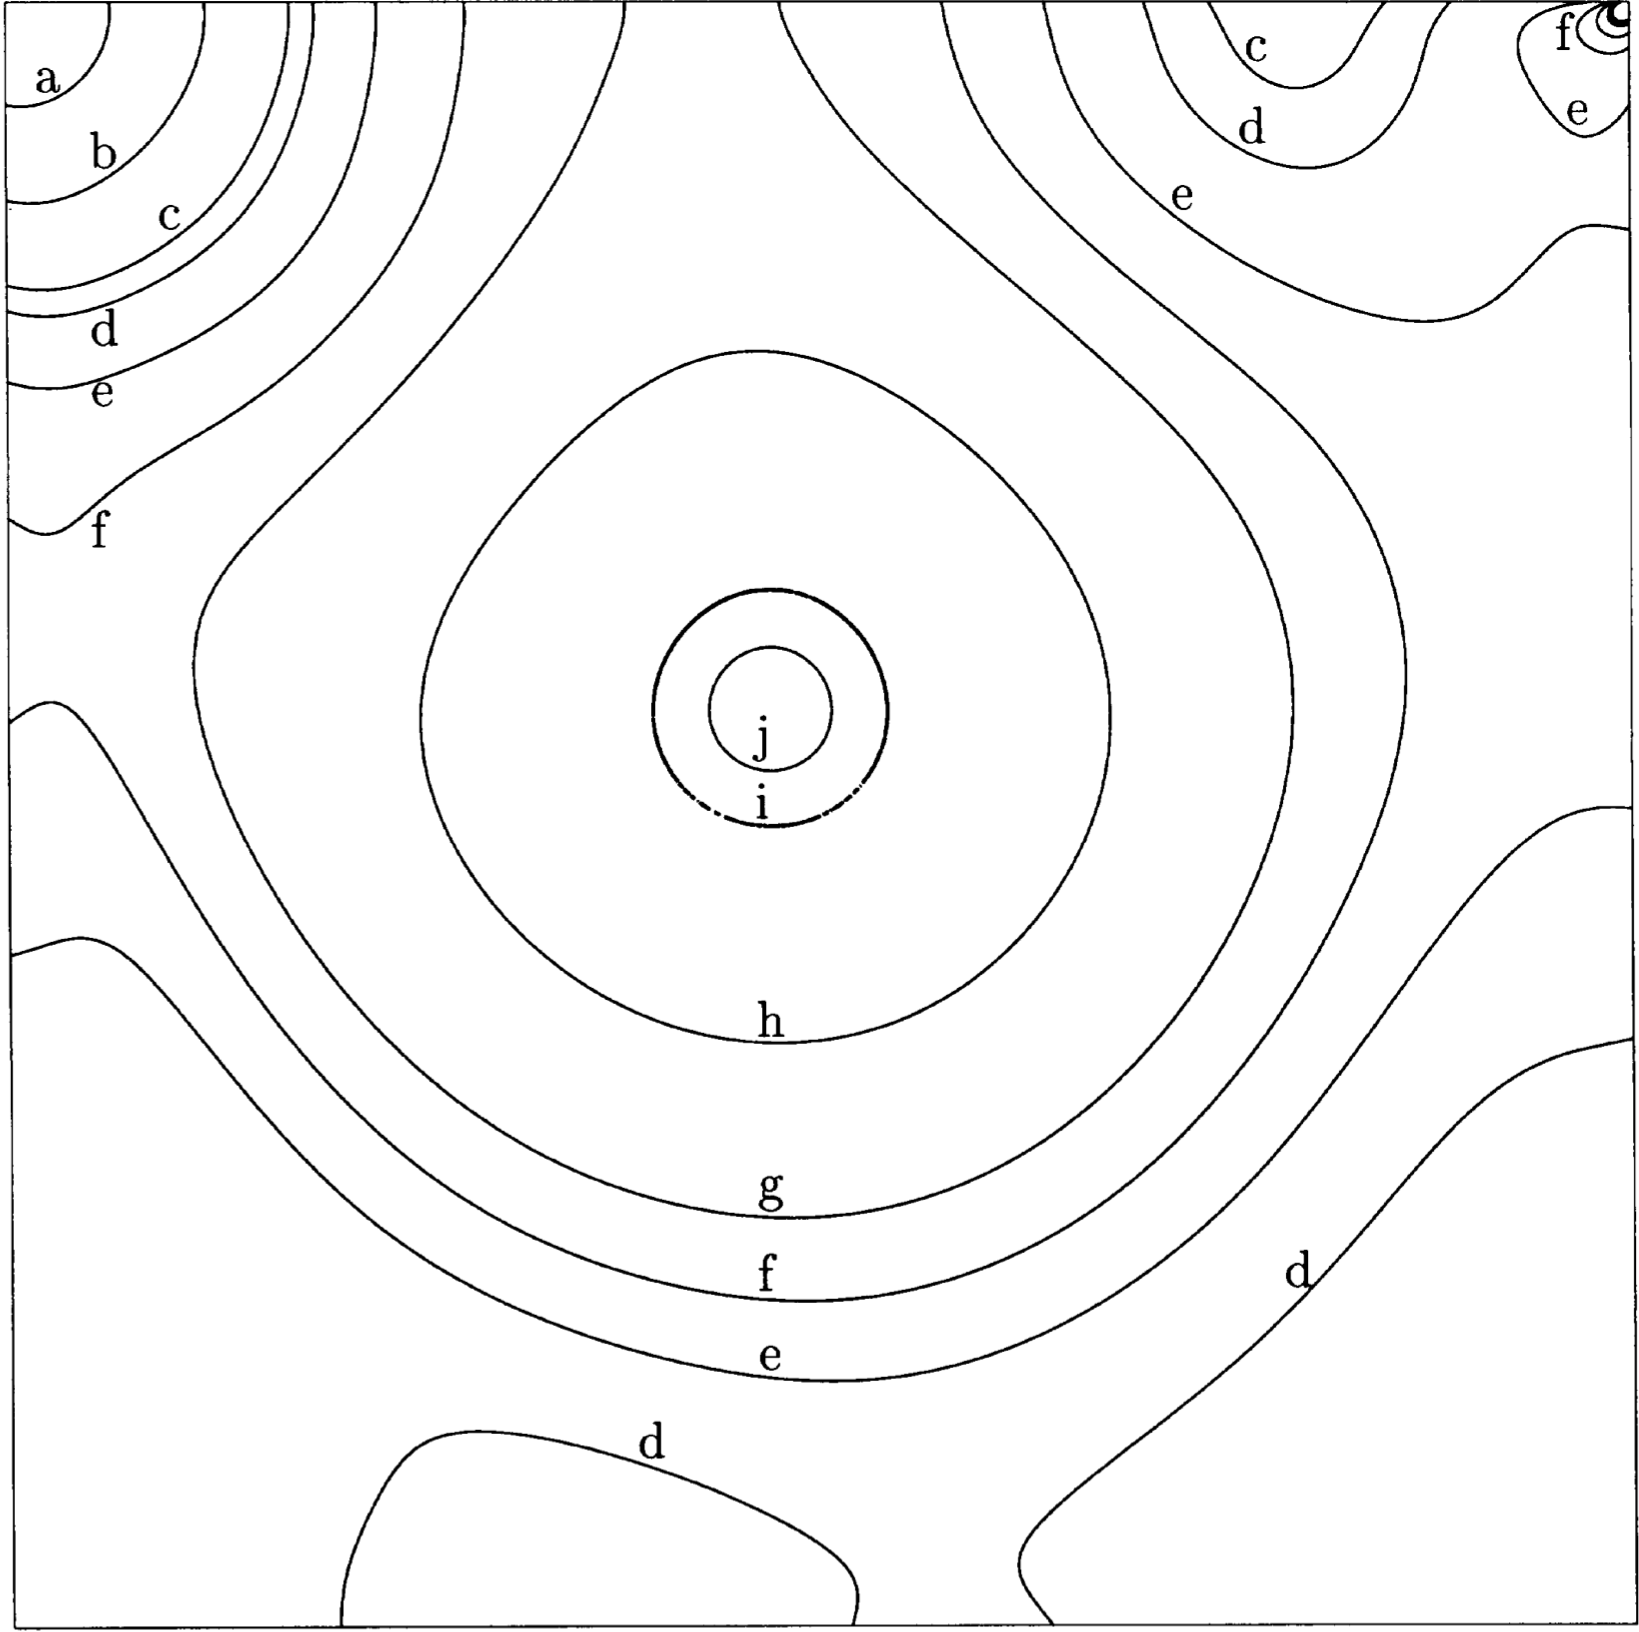
\includegraphics[width=0.95\linewidth]{Images/pressure.png}}
	    \caption{Benchmark}
    	\label{fig:pressurea}
    \end{subfigure}
    % This comment avoids line break...
    \begin{subfigure}[b]{0.49\textwidth}
        \centering{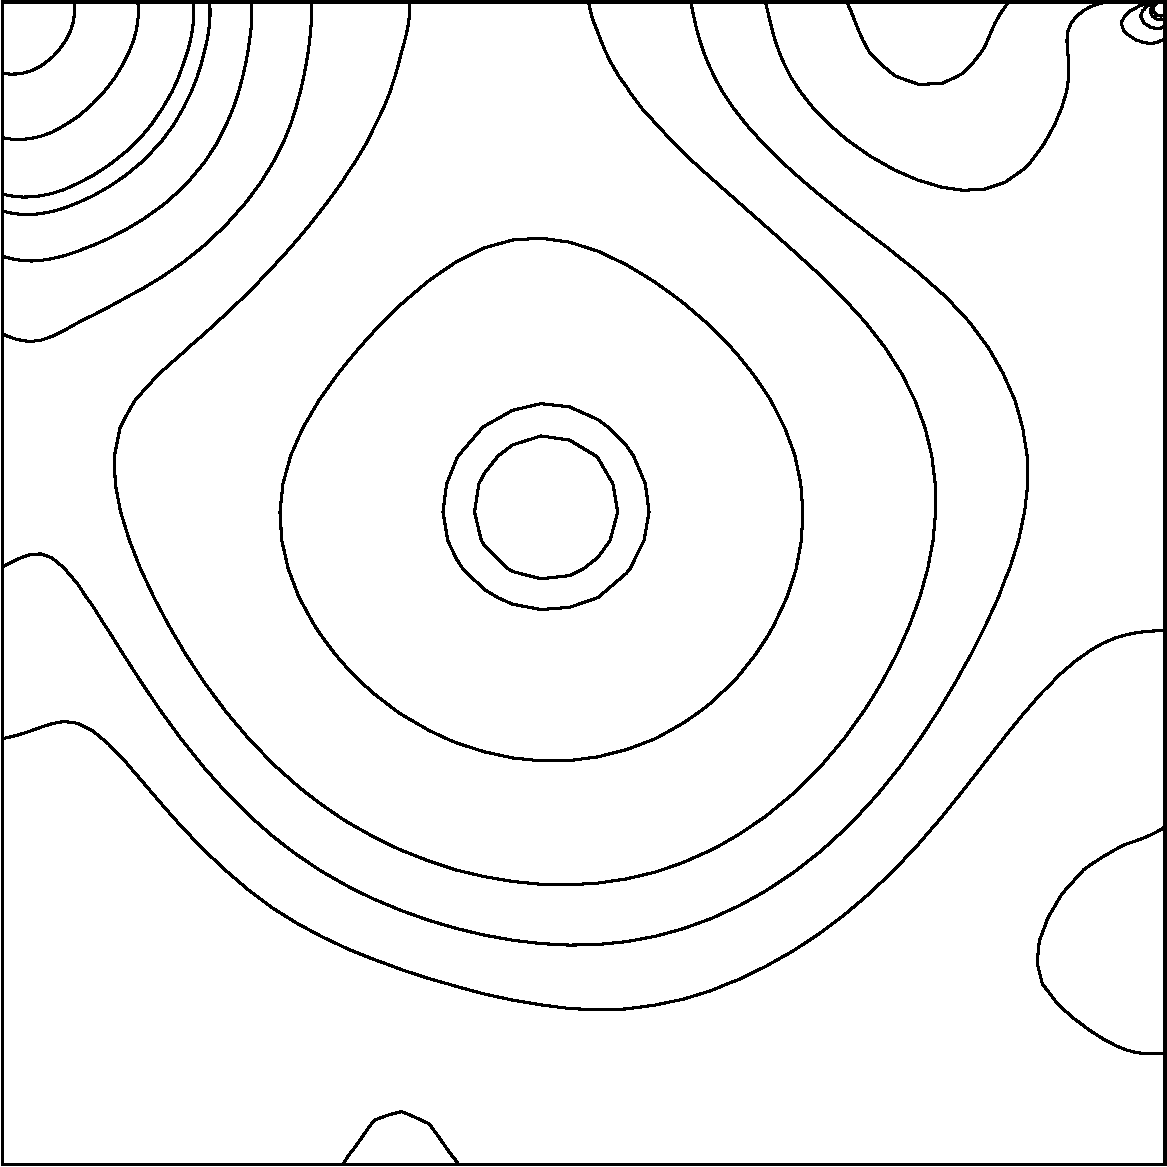
\includegraphics[width=0.95\linewidth]{Images/pressure64.pdf}}
	    \caption{$N = 64$}
	    \label{fig:pressureb}	
    \end{subfigure}
    
    \vspace{1cm}
    
    \begin{subfigure}[b]{0.49\textwidth}
        \centering{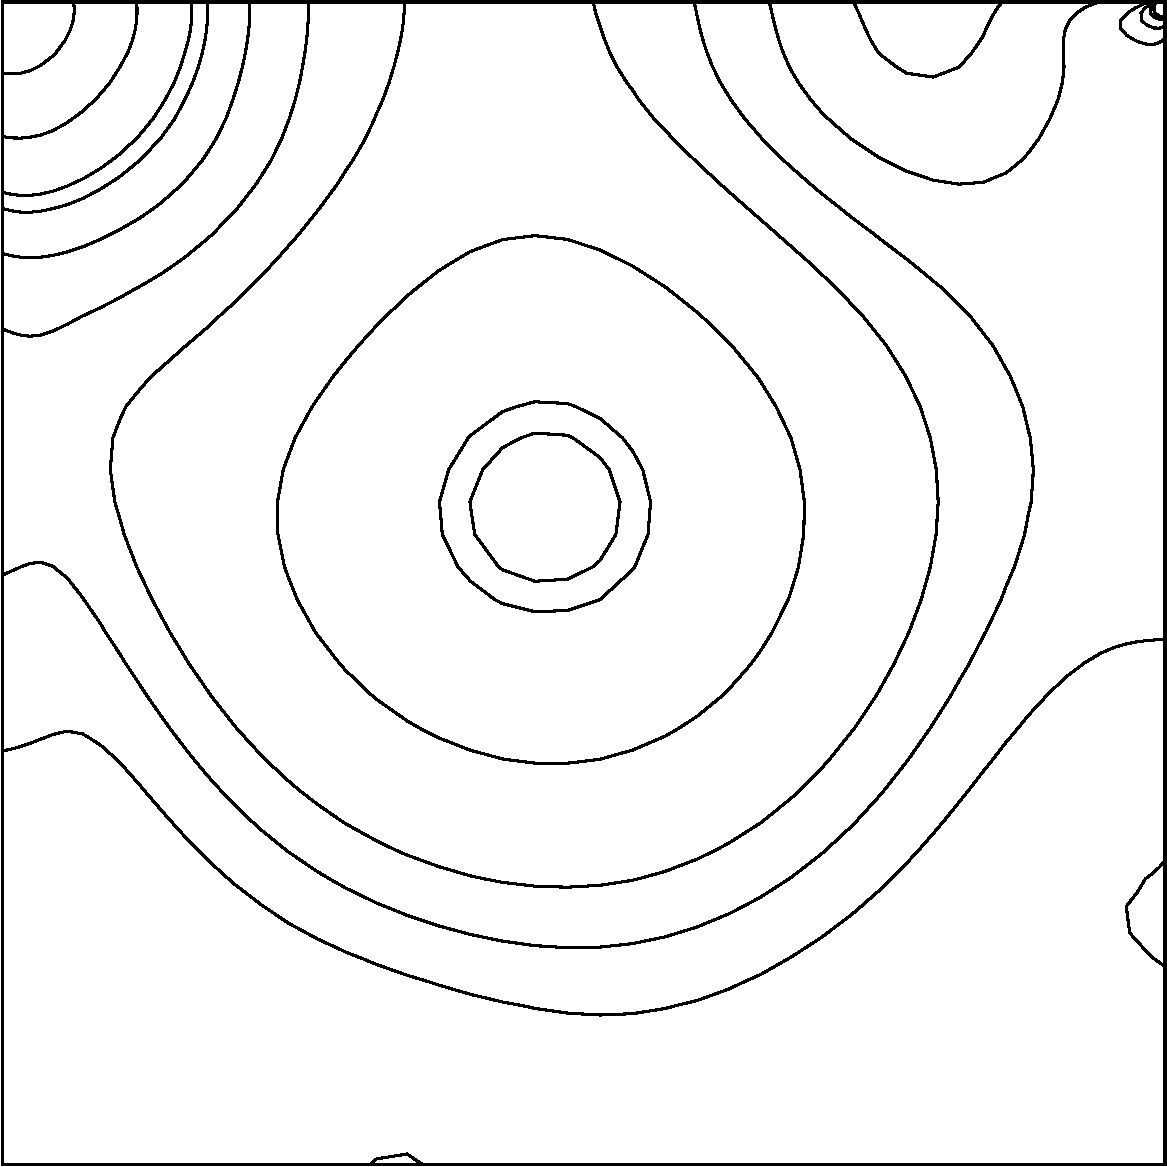
\includegraphics[width=0.95\linewidth]{Images/pressure56.pdf}}
	    \caption{$N = 56$}
    	\label{fig:pressurec}
    \end{subfigure}
    % This comment avoids line break...
    \begin{subfigure}[b]{0.49\textwidth}
        \centering{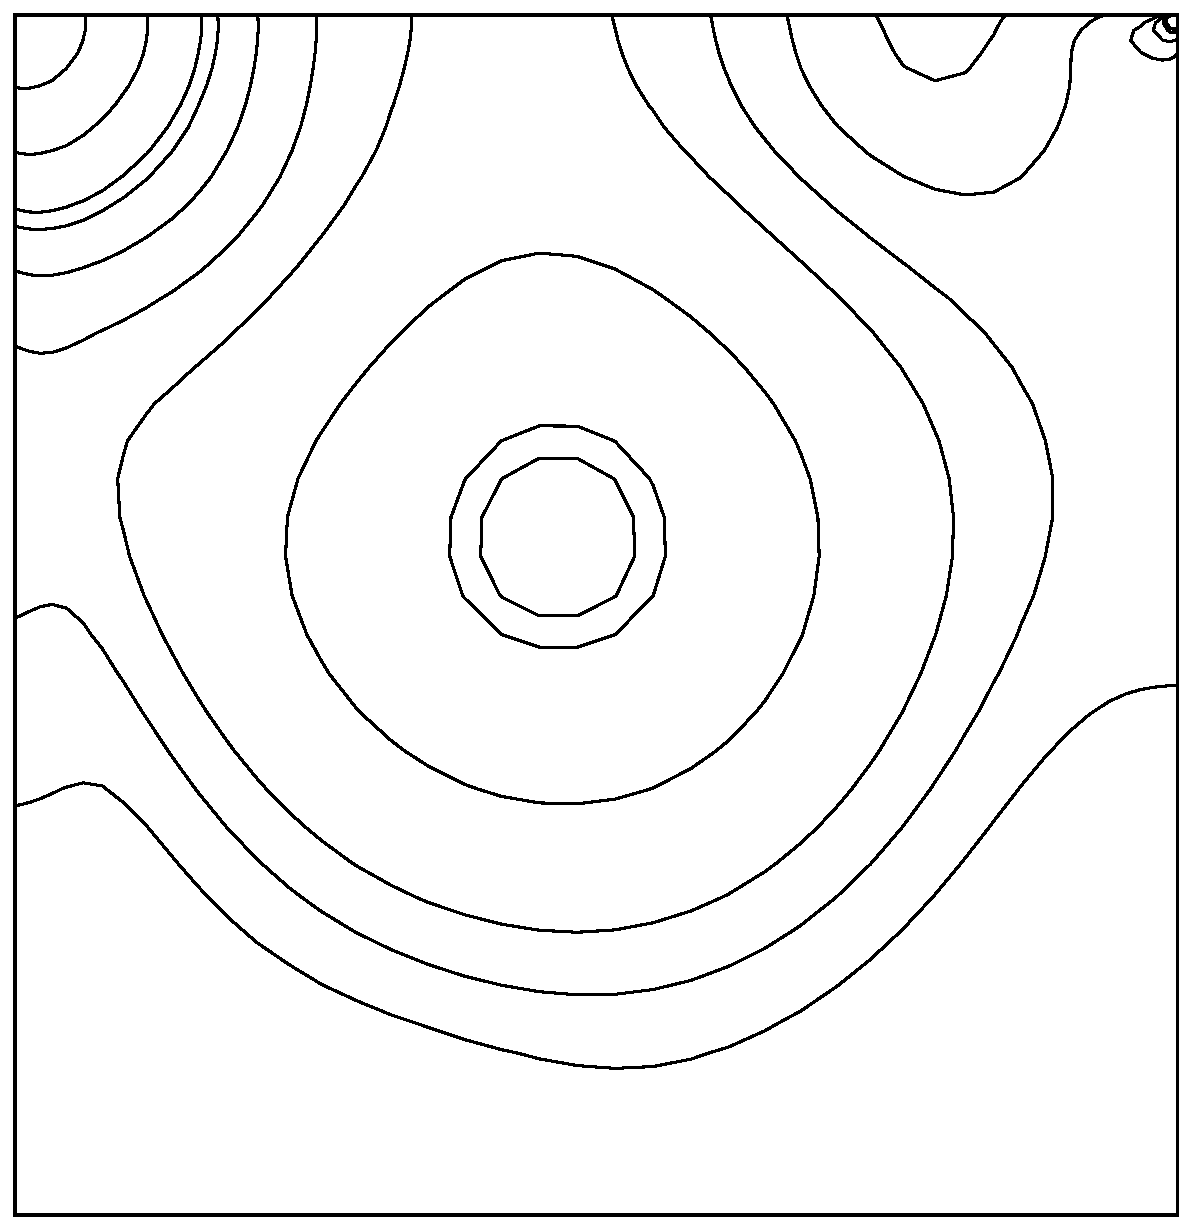
\includegraphics[width=0.95\linewidth]{Images/pressure48.pdf}}
	    \caption{$N = 48$}
	    \label{fig:pressured}	
    \end{subfigure}
    
    \vspace{1cm}
    
    \begin{subfigure}[b]{0.49\textwidth}
        \centering{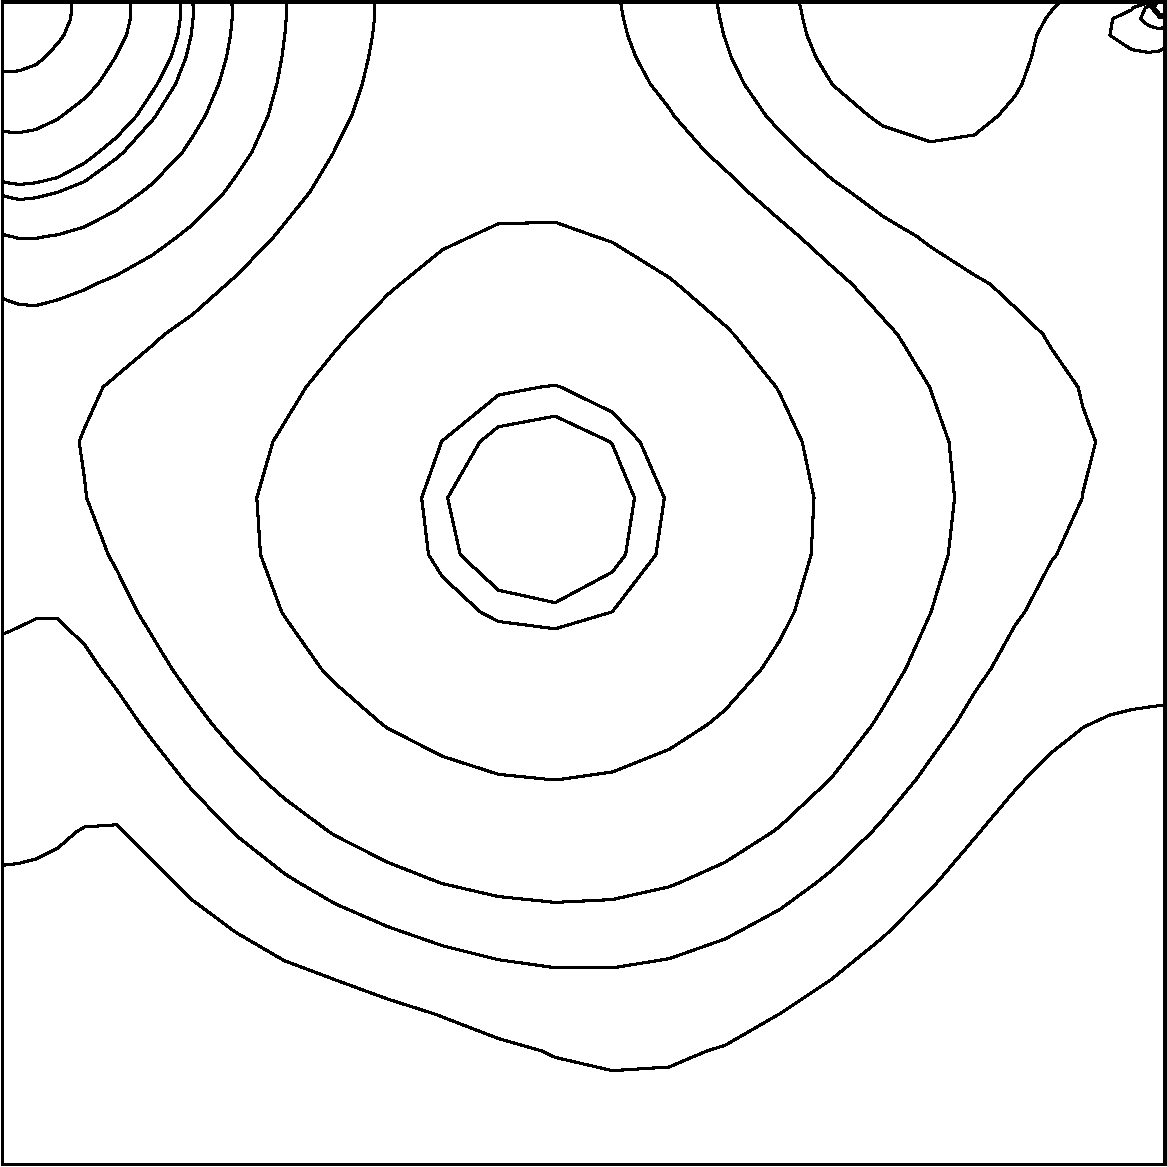
\includegraphics[width=0.95\linewidth]{Images/pressure32.pdf}}
	    \caption{$N = 32$}
    	\label{fig:pressuree}
    \end{subfigure}
    % This comment avoids line break...
    \begin{subfigure}[b]{0.49\textwidth}
        \centering{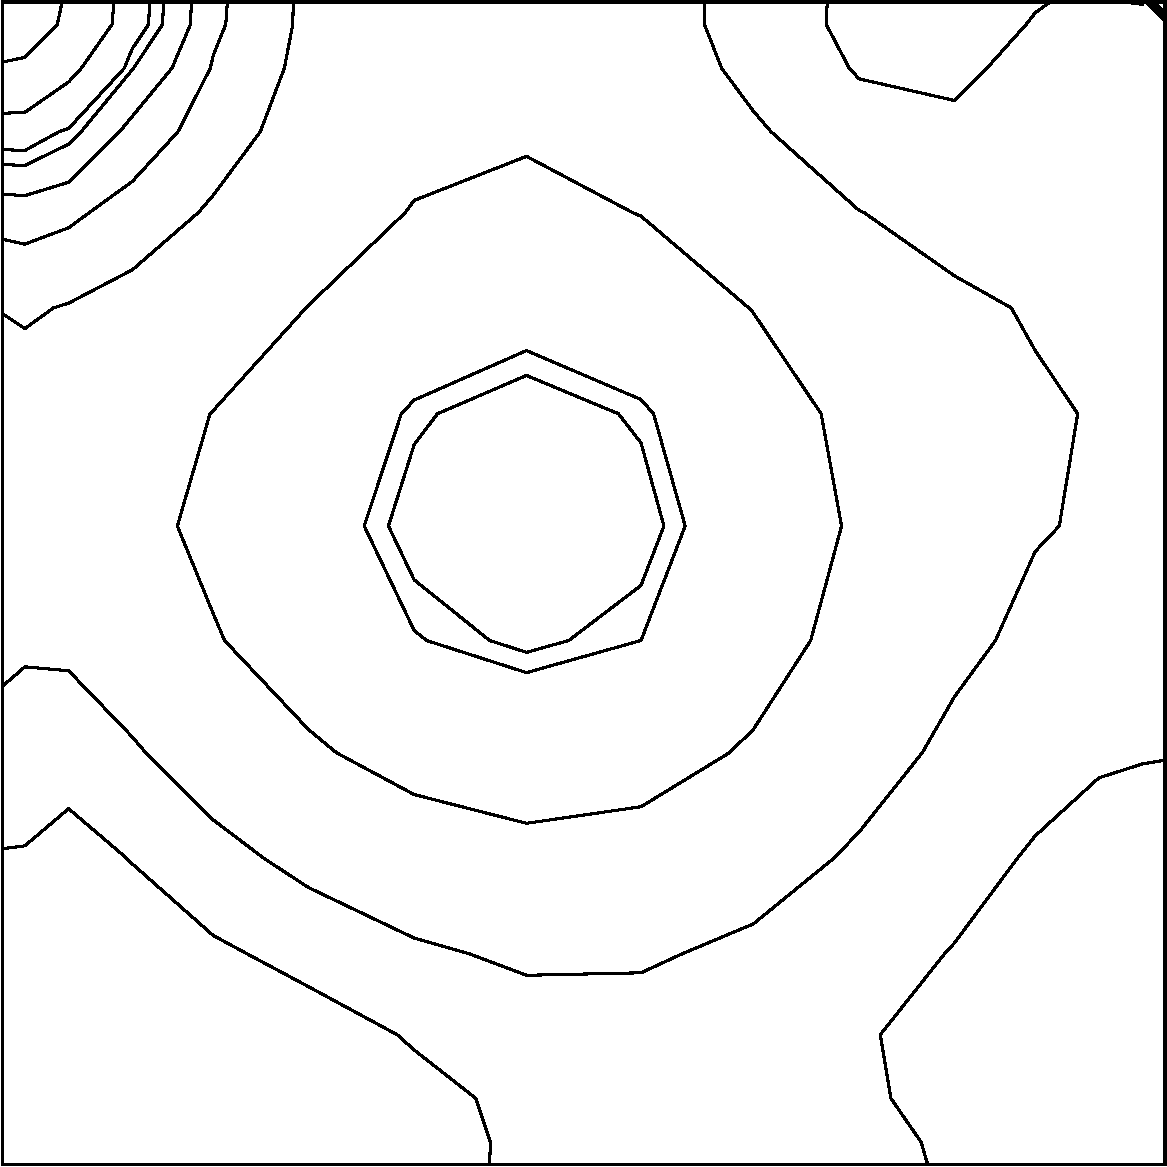
\includegraphics[width=0.95\linewidth]{Images/pressure16.pdf}}
	    \caption{$N = 16$}
	    \label{fig:pressuref}
    \end{subfigure}
    \caption{Static pressure for $\text{Re} = 1000$, $\Delta t = 0.0002$, $\text{tol} = 1 \cdot 10^{-5}$, and various values of $N$ as well as the benchmark result.}
    \label{fig:allpressure}
\end{figure}


\chapter{Conclusion}
\label{cha:conclusion}

\begin{figure}[p]
    \centering
    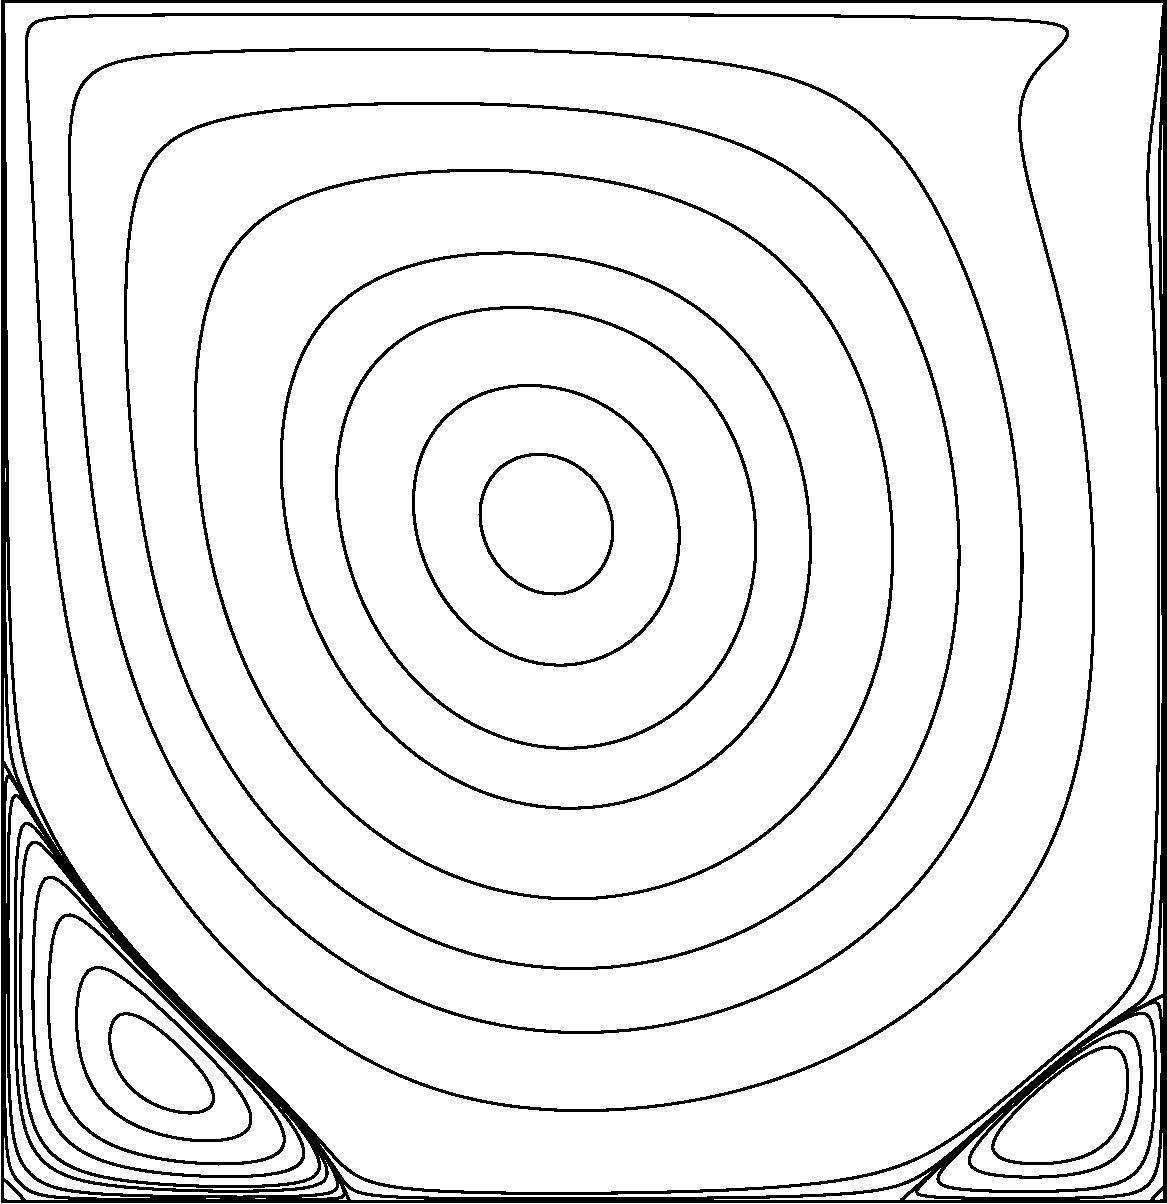
\includegraphics[width=0.8\textwidth]{Images/streamFunction.pdf}
    \caption{Awesome Image}
    \label{fig:awesome_image}
\end{figure}

\begin{figure}[p]
    \centering
    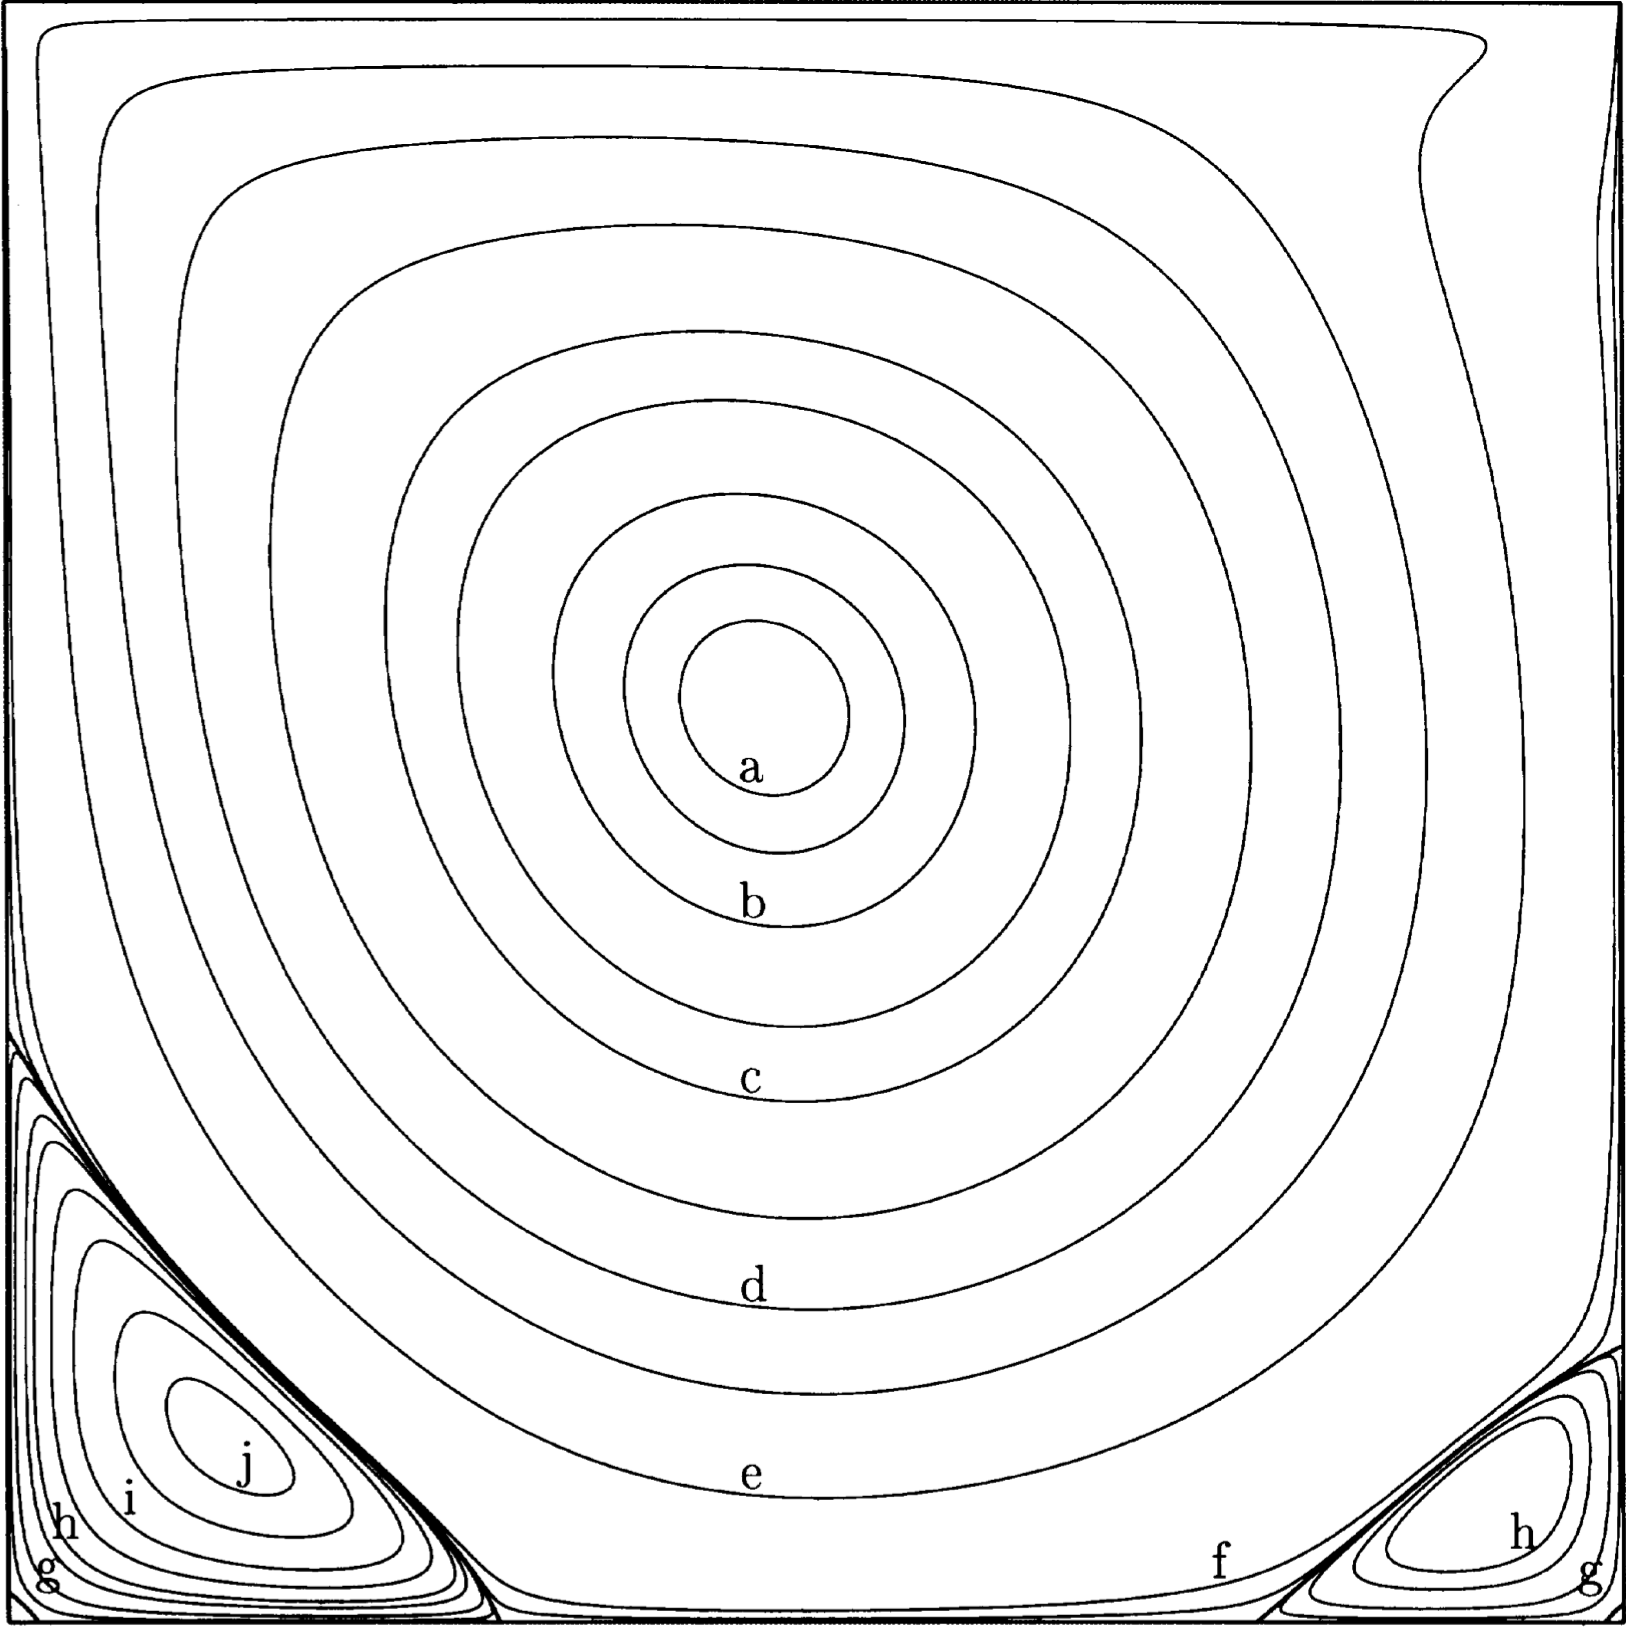
\includegraphics[width=0.8\textwidth]{Images/streamFunction.png}
    \caption{Awesome Image}
    \label{fig:awesome_image}
\end{figure}

\begin{figure}[p]
    \centering
    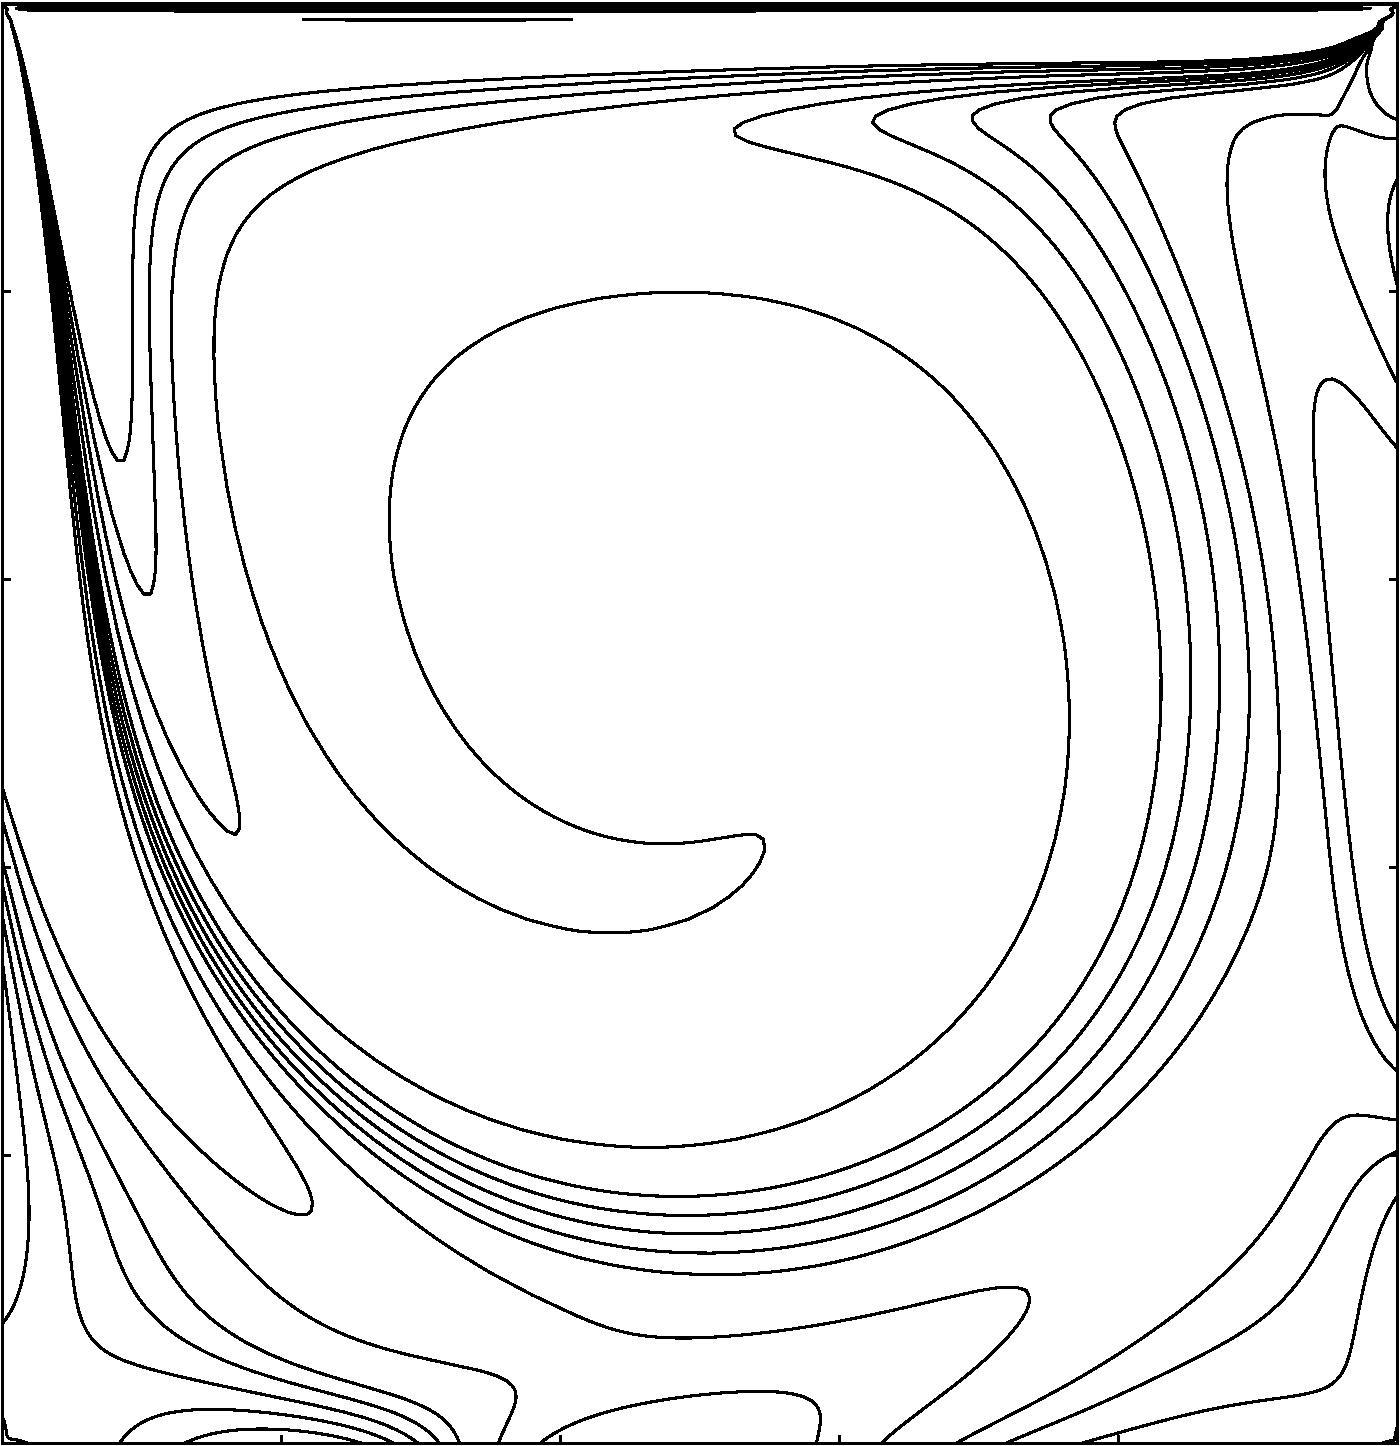
\includegraphics[width=0.8\textwidth]{Images/vorticity.pdf}
    \caption{Awesome Image}
    \label{fig:awesome_image}
\end{figure}

\begin{figure}[p]
    \centering
    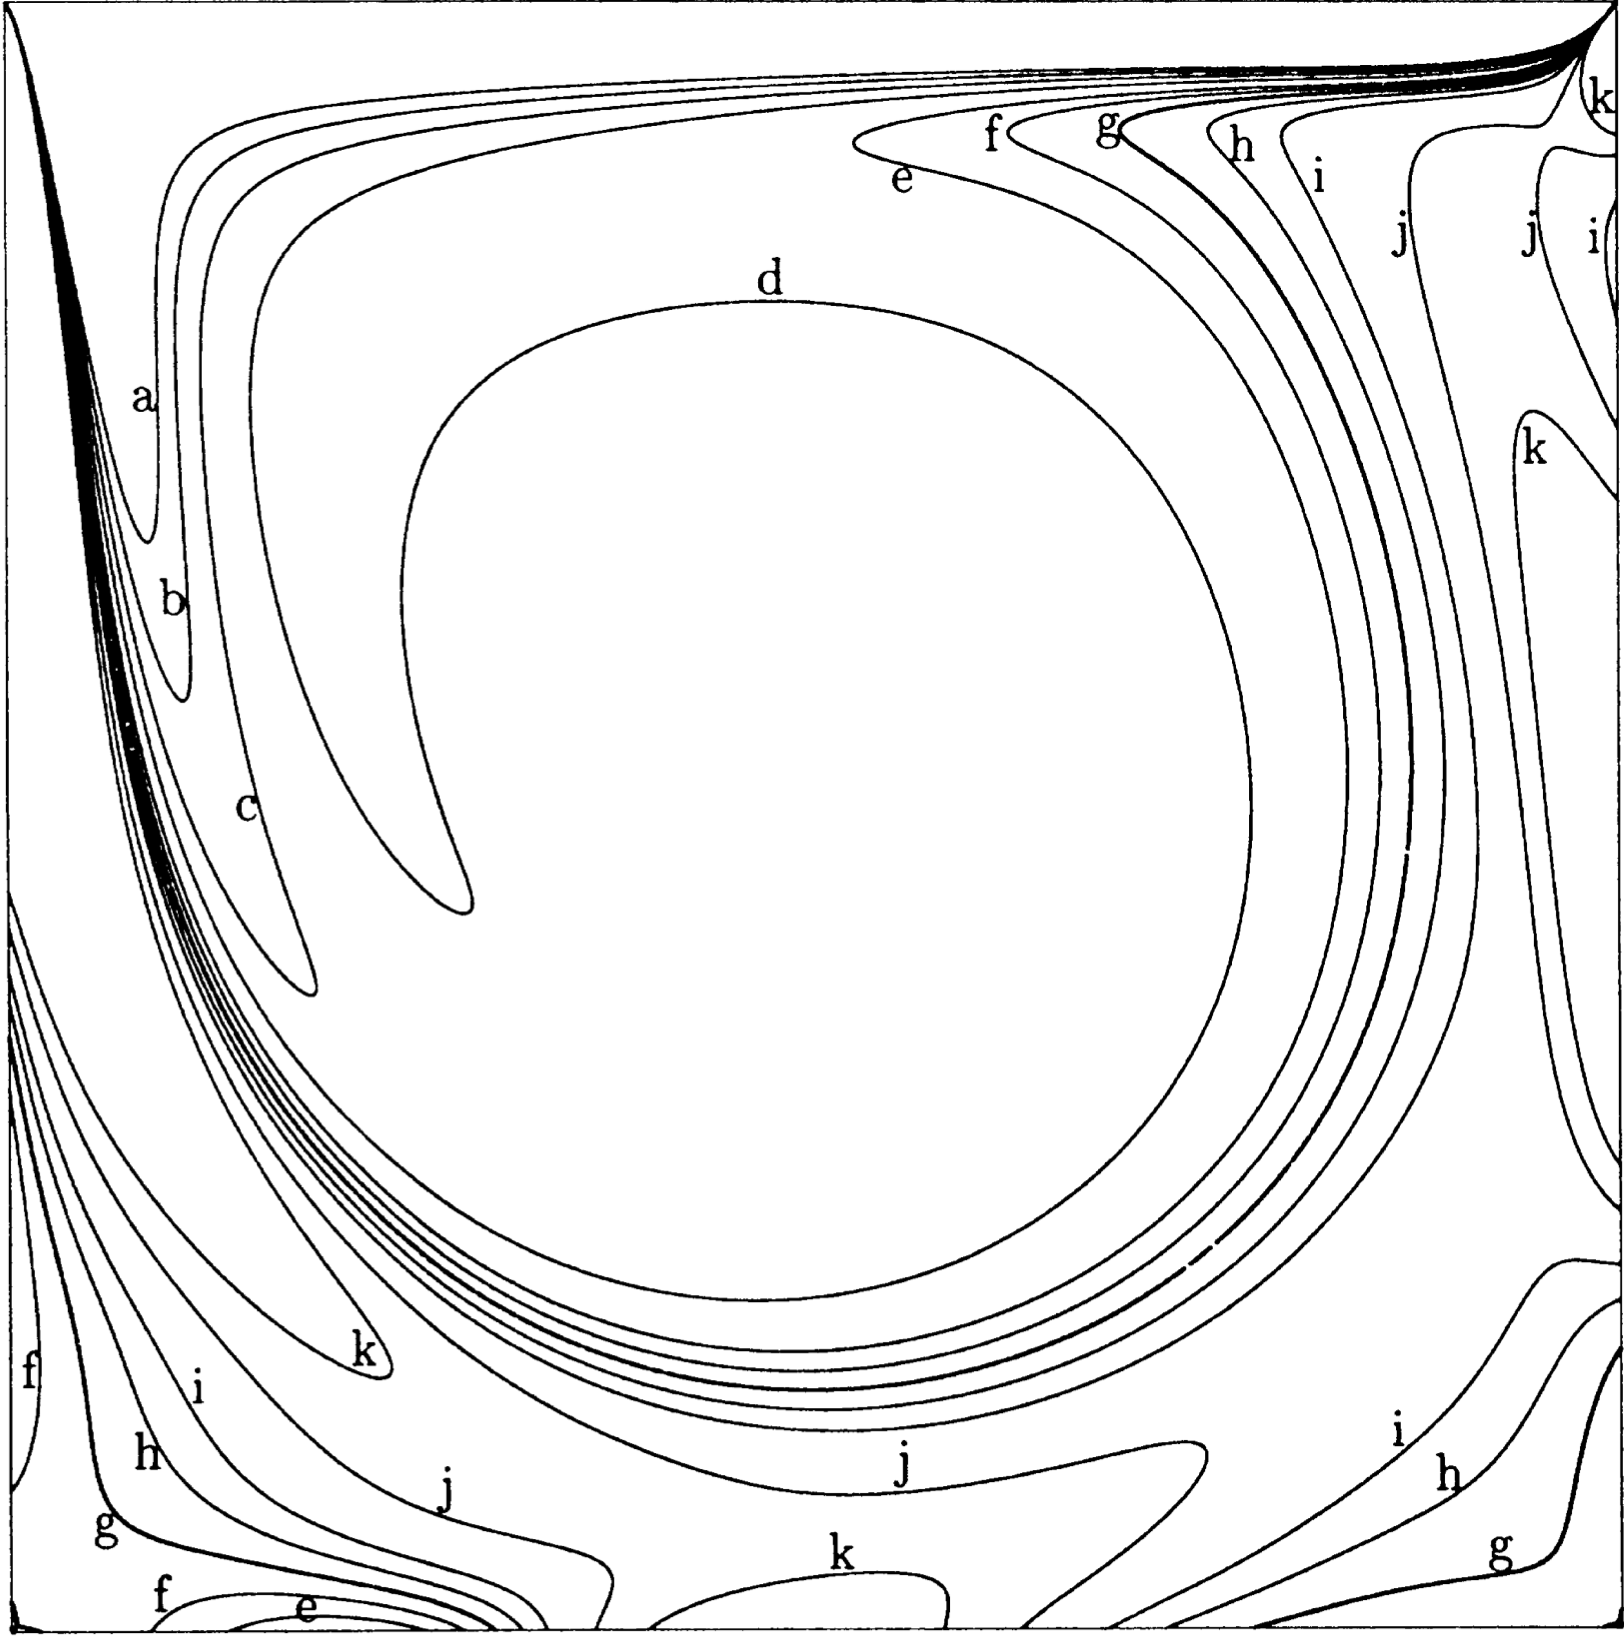
\includegraphics[width=0.8\textwidth]{Images/vorticity.png}
    \caption{Awesome Image}
    \label{fig:awesome_image}
\end{figure}

\begin{figure}[p]
    \centering
    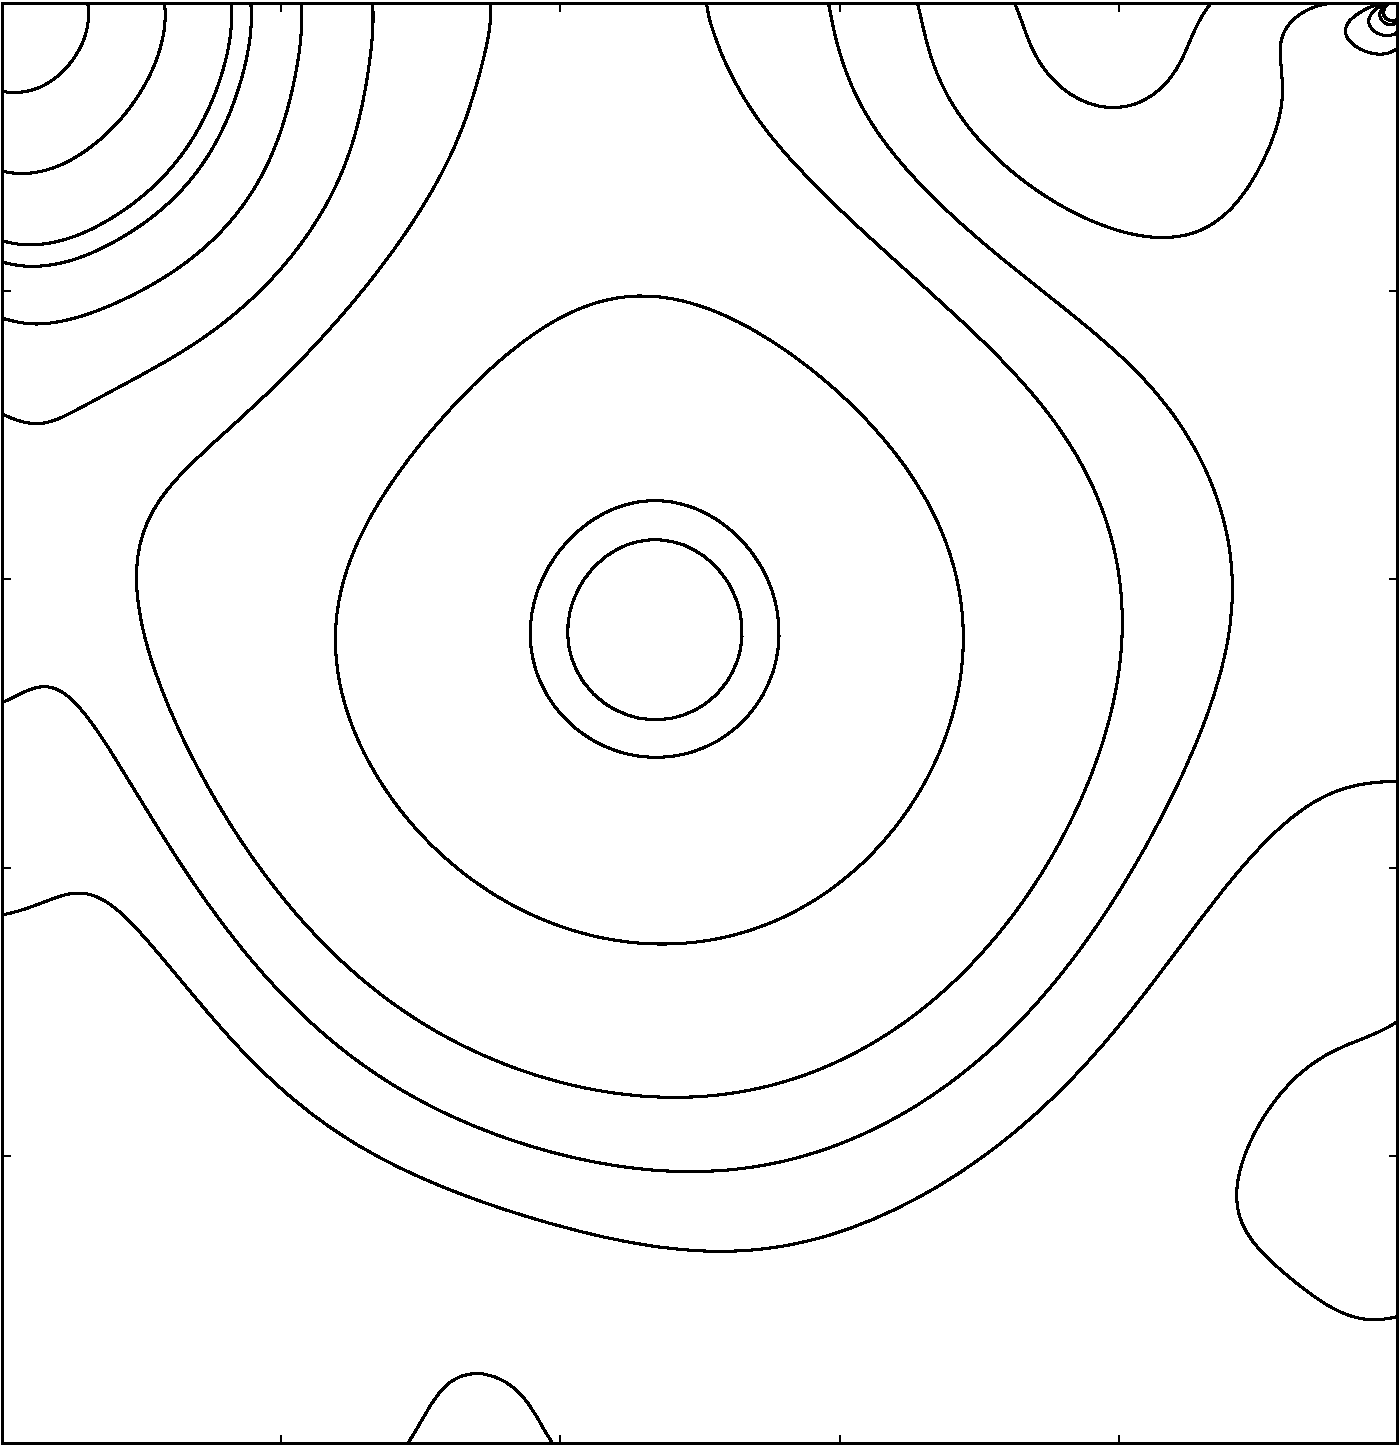
\includegraphics[width=0.8\textwidth]{Images/pressure.pdf}
    \caption{Awesome Image}
    \label{fig:awesome_image}
\end{figure}

\begin{figure}[p]
    \centering
    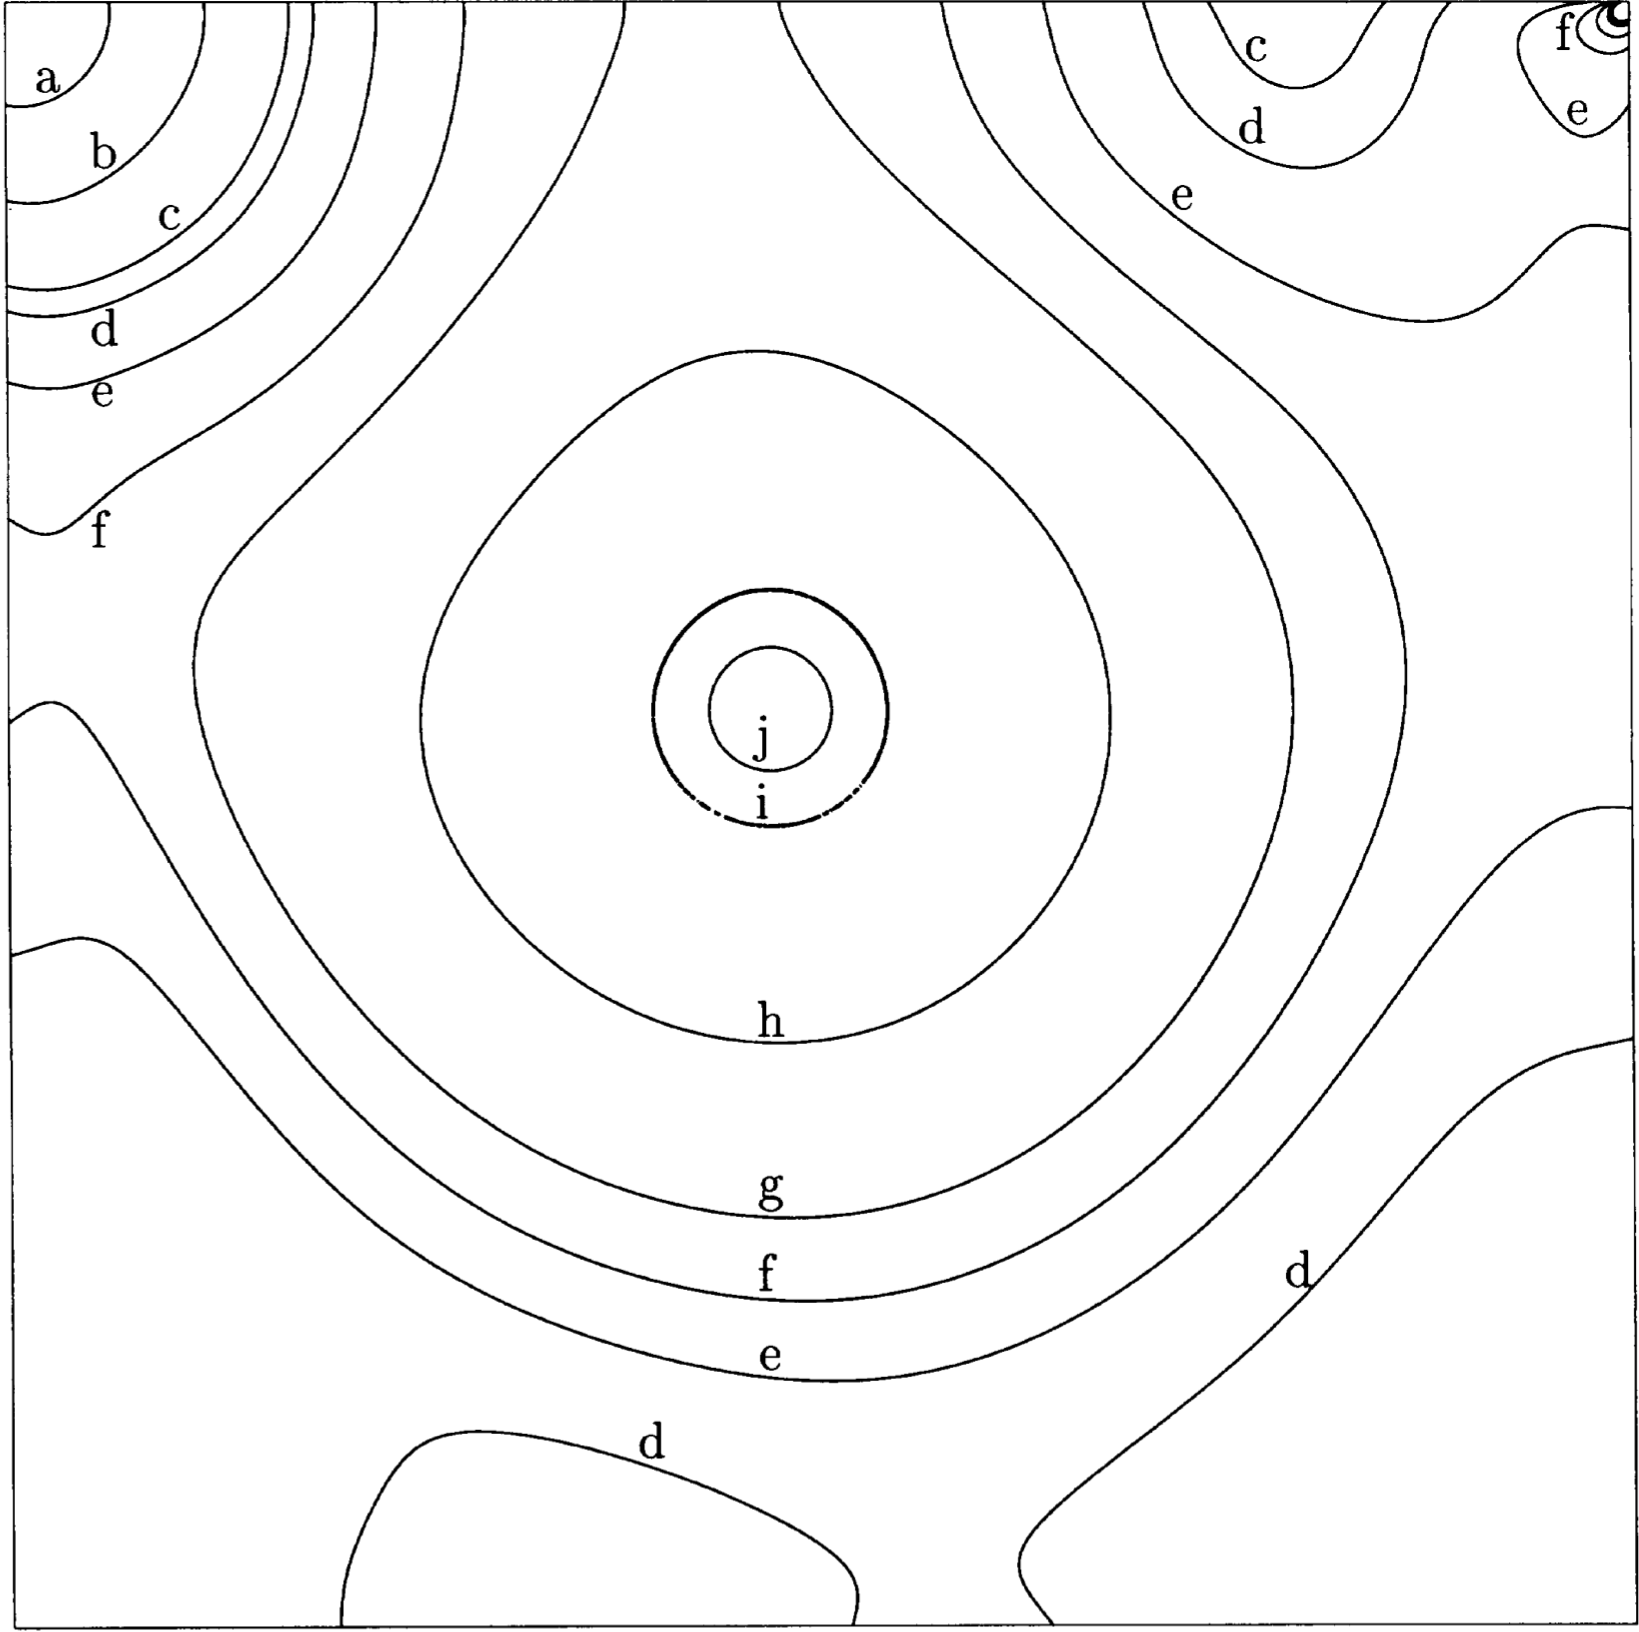
\includegraphics[width=0.8\textwidth]{Images/pressure.png}
    \caption{Awesome Image}
    \label{fig:awesome_image}
\end{figure}

\printbibliography[heading=bibintoc, title={References}]

\end{document}
